
\chapter{Danish Housing Prices}
\label{ch:housing_price_analysis}
\epigraph{\textit{``Buy land, they’re not making it anymore.''}}{--- Mark Twain}
% \epigraph{\textit{``It’s tangible, it’s solid, it’s beautiful. It’s artistic, from my standpoint, and I just love real estate.''}}{--- Donald Trump}
\newthought{Housing markets} have always been a playing field for economists, property speculators, real estate agents, and realtors. The author of this thesis is by no metric any of these, not even close to, yet, when the issue of estimating Danish housing prices came up, it was too much of a challenge just lying there to let it go. Estimating housing prices is a classical economical discipline as seen in papers from the Danish National Bank developing a regional model of the Danish housing market \autocite{hviidWorkingPaperRegional2017} to an analysis of the financial crisis in \num{2008}-\num{2009} and its effects on the Copenhagen metropolitan area \autocite{mulalicFinancialCrisisDiverging2017}. 

\begin{figure}
  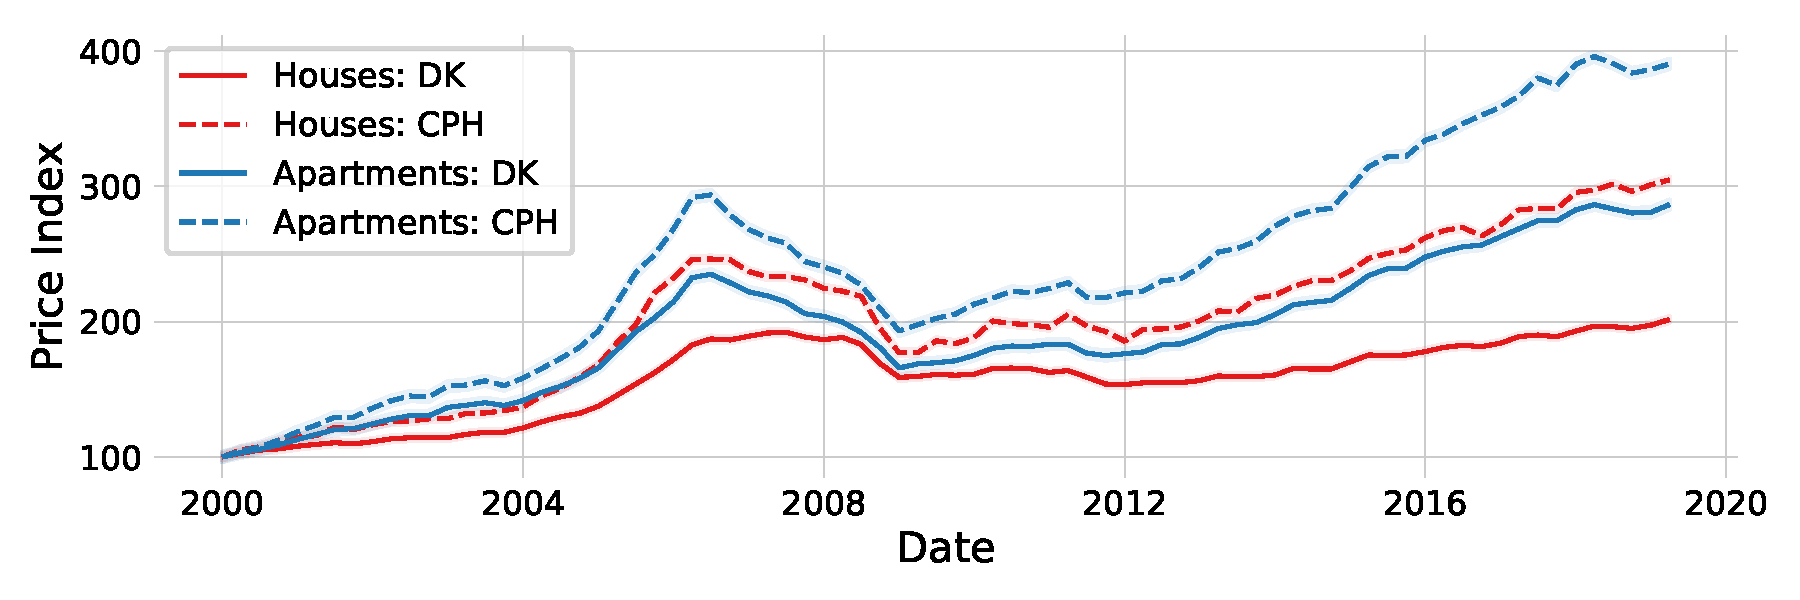
\includegraphics[width=0.98\textwidth, trim=10 15 10 10, clip]{figures/housing_price_index_dst/housingindex_wide.pdf}
  \caption[Danish Housing Price Index]
          {Price Index of the Danish housing market. Prince index of Danish one-family houses and owner-occupied apartments where \textcolor{red}{houses} are shown in red and \textcolor{blue}{apartments} in blue, where full lines are for the entirety of Denmark and dashed lines are only for Copenhagen. Errorbars (scaled up with a factor of 2) are shown as colored bands. The price index and its uncertainty is based on numbers from \citet{dstPriceIndexEJ14}, however, rescaled to 100 in 2000 (instead of 2006 as it was in the data).}
  \label{fig:h:price_index}
\end{figure}

If one takes a look at the time development of the Danish housing market, the Danish governmental organization for statistics, Statistics Denmark, releases a price index \citep{dstPriceIndexEJ14} for both one-family houses (OFH) and owner-occupied apartments (OOA) quarterly, see Figure~\ref{fig:h:price_index}. Here it is easy to see the effect of the financial crisis around 2008, but also the steady increase in the housing market in both Copenhagen and the entire country since then. Housing in this context means both actual houses and privately owned apartments, and will be called residences in general in this project. 

The goal of this subproject is not to predict any future collapse as the financial markets as we saw upwards of 10 years ago. Instead, it is to learn patterns in the price of houses in steady times. The goal is training a computer to automatically find these patterns and see if we can improve this model\sidenote{In contrary to \citet{hviidWorkingPaperRegional2017, mulalicFinancialCrisisDiverging2017} and others who base their models on macro-economic principles.}.

In \autoref{sec:h:data_cleaning} the data will be introduced and feature augmented in \autoref{sec:h:feature_augmentation}.  The evaluation functions will be discussed in \autoref{sec:h:evaluation_function} and the choice of loss function decided in \autoref{sec:h:initial_hyperparameter_optimization}. The model is fitted and optimized in \autoref{sec:h:hyperparamater_optimization} and the results presented in \autoref{sec:h:results}. Finally the model will be further understood in \autoref{sec:h:model_inspection}, some additional models presented in \autoref{sec:h:multiple_models} and at last the models will be discussed in \autoref{sec:h:discussion}.

\section{Data Preparation and Exploratory Data Analysis}
\label{sec:h:data_cleaning}
\epigraph{\textit{``\SI{80}{\percent} of data science is cleaning the data and \SI{20}{\percent} is complaining about cleaning the data.''}}{--- Anthony Goldbloom, Kaggle}


The first part of any data science project is actually getting the data and being able to read it. This has been an iterative process that has improved over time. The last data transfer we got was September \nth{3} 2019 which consisted of a \SI{522.4}{\mega\byte} CSV file with dimensions $(\num{711212}, \num{171})$. This section will go through the data cleaning process.

Before any further data analysis is performed, all of the data is loaded, except columns which only contain internal information for Boligsiden\sidenote{The variables \code{Sag_Kvhx}, \code{Enhed_GOP_BoligtypeKode}, and \code{Bygning_GOP_Matrikelnr}.}. To get a better understanding of all of the variables, histograms showing the one-dimensional distributions of all of the variables were made.

Four particularly interesting ones are seen in Figure~\ref{fig:h:variable_overview}: 
the distribution of the date of the sale \code{SalgsDato} in subfigure~\subref{fig:h:variable_overview_date},  
the distribution of the type of residence \code{SagtypeNr} in subfigure~\subref{fig:h:variable_overview_type},
the distribution of the longitude of the residence \code{GisX_WGS84} in subfigure~\subref{fig:h:variable_overview_longitude}, and
the distribution of the area of the residence \code{ArealBolig} in subfigure~\subref{fig:h:variable_overview_area}.

\begin{figure*}
  \centering
  % \vspace*{-\abovecaptionskip}
  \subfloat[\label{fig:h:variable_overview_date}]{\qquad}
  \includegraphics[width=0.45\textwidth, page=2, trim=15 15 15 15, clip]{figures/housing/overview_fig.pdf}\hfil
  \subfloat[\label{fig:h:variable_overview_type}]{\qquad}
  \includegraphics[width=0.45\textwidth, page=6, trim=15 15 15 15, clip]{figures/housing/overview_fig.pdf}
  \subfloat[\label{fig:h:variable_overview_longitude}]{\qquad}
  \includegraphics[width=0.45\textwidth, page=20, trim=15 15 15 15, clip]{figures/housing/overview_fig.pdf}\hfil
  \subfloat[\label{fig:h:variable_overview_area}]{\qquad}
  \includegraphics[width=0.45\textwidth, page=23, trim=15 15 15 15, clip]{figures/housing/overview_fig.pdf}
  \caption[Distributions of the Variables in the Housing Prices]{Distributions of four out of the \num{168} input variables. 
           Subplot ~\protect\subref{fig:h:variable_overview_date} shows the date of the sale, 
           Subplot ~\protect\subref{fig:h:variable_overview_type} shows the type of residence,
           Subplot ~\protect\subref{fig:h:variable_overview_longitude} shows the longitude,
           Subplot ~\protect\subref{fig:h:variable_overview_area} shows the area og the house.}
  \label{fig:h:variable_overview}
  \vspace{\abovecaptionskip}
\end{figure*}

The distribution of the date of sale, Figure~\ref{fig:h:variable_overview} \subref{fig:h:variable_overview_date}, is an interesting variable because it shows how Boligsiden has been collecting more and more data over time. Here \num{2007} and \num{2019} are clear outliers since their current database only contains sales from the end of \num{2007}, and \num{2019} only contains data from the first eight months of the year. The \code{SagTypeNr} is a discrete code that Boligsiden uses to differentiate between different types of residences. The mapping between code and description is shown in Table~\ref{tab:h:salgstype}. 

\begin{margintable}
  \centering
  \begin{tabular}{@{}rl@{}}
  % \toprule
  Type & Name           \\ 
  \midrule
  100  & Villa          \\ 
  200  & Rækkehus       \\
  300  & Ejerlejlighed  \\
  400  & Fritidsbolig   \\
  401  & Kolonihave     \\
  500  & Andelsbolig    \\
  600  & Landejendom    \\
  700  & Helårsgrund    \\
  800  & Fritidsgrund   \\
  900  & Villalejlighed \\
  1000 & Kvæggård       \\
  1100 & Svinegård      \\
  1200 & Planteavlsgård \\
  1300 & Skovejendom    \\
  1400 & Lystejendom    \\
  1500 & Specialejendom \\ 
  % \bottomrule
  \end{tabular}
  \vspace{\abovecaptionskip}
  \caption[Mapping between the Code in \code{SagTypeNr} and the Type of Residence]{Mapping between the code in \code{SagTypeNr} and the type of residence. The two important types of residences are villa (one-family houses) and ejerlejlighed (owner-occupied apartments).}
  \label{tab:h:salgstype}
\end{margintable}

In this project only one-family houses -- \q{Villas} in Danish -- with code \num{100} and owner-occupied apartments -- \q{Ejerlejlighed} in Danish -- with code \num{300} are considered. In Figure~\ref{fig:h:variable_overview} \subref{fig:h:variable_overview_type} it is shown that these two types of residences are also the most frequent sales with close to \num{400000} and \num{150000} sales in total. The longitude distribution, Figure~\ref{fig:h:variable_overview} \subref{fig:h:variable_overview_longitude}, is mostly interesting due to fact that it clearly shows how the Great Belt and especially the Baltic Sea separates Denmark into three parts; the Western part, the Eastern part, and then Bornholm. Note that more than \SI{5}{\percent} of the residences' locations are unknown values, so-called \q{Not A Number}s (NANs). The distribution of the area, Figure~\ref{fig:h:variable_overview} \subref{fig:h:variable_overview_area}, shows that most residences are between \SI{50}{\meter^2} and \SI{200}{\meter^2}, as expected in Denmark. However, a relatively large part of the residences, \SI{2.5}{\percent}, are listed as having an area of \SI{0}{\meter^2} which are obviously erroneous entries. All of the 1D-distributions are shown in Figure~\ref{fig:h:variable_overview_all_1}--\ref{fig:h:variable_overview_all_14}. 

The geographic distribution of sales are shown in Figure~\ref{fig:h:geo_overview}. The residences are coloured according the square meter price in Figure~\ref{fig:h:geo_overview} \subref{fig:h:geo_overview_sqm_price} and according to the sales price in Figure~\ref{fig:h:geo_overview} \subref{fig:h:geo_overview_sales_price}. Notice the strong correlation between the distance to water and the square meter price, a correlation that is less visible when looking at the sales price. Since these plots each contain \num{674647} points\sidenote{Only sales with a valid GPS-coordinate and area of residence are shown}, over-plotting quickly becomes an issue. To circumvent this the software package called DataShader \autocite{bednarDatashaderRevealingStructure2019} was used which in a simple, consistent, and not at least computationally efficient manner allows one to plot big data.

\begin{figure*}
  \centering
  % \vspace*{-\abovecaptionskip}
  \subfloat[\label{fig:h:geo_overview_sqm_price}]{\,}
  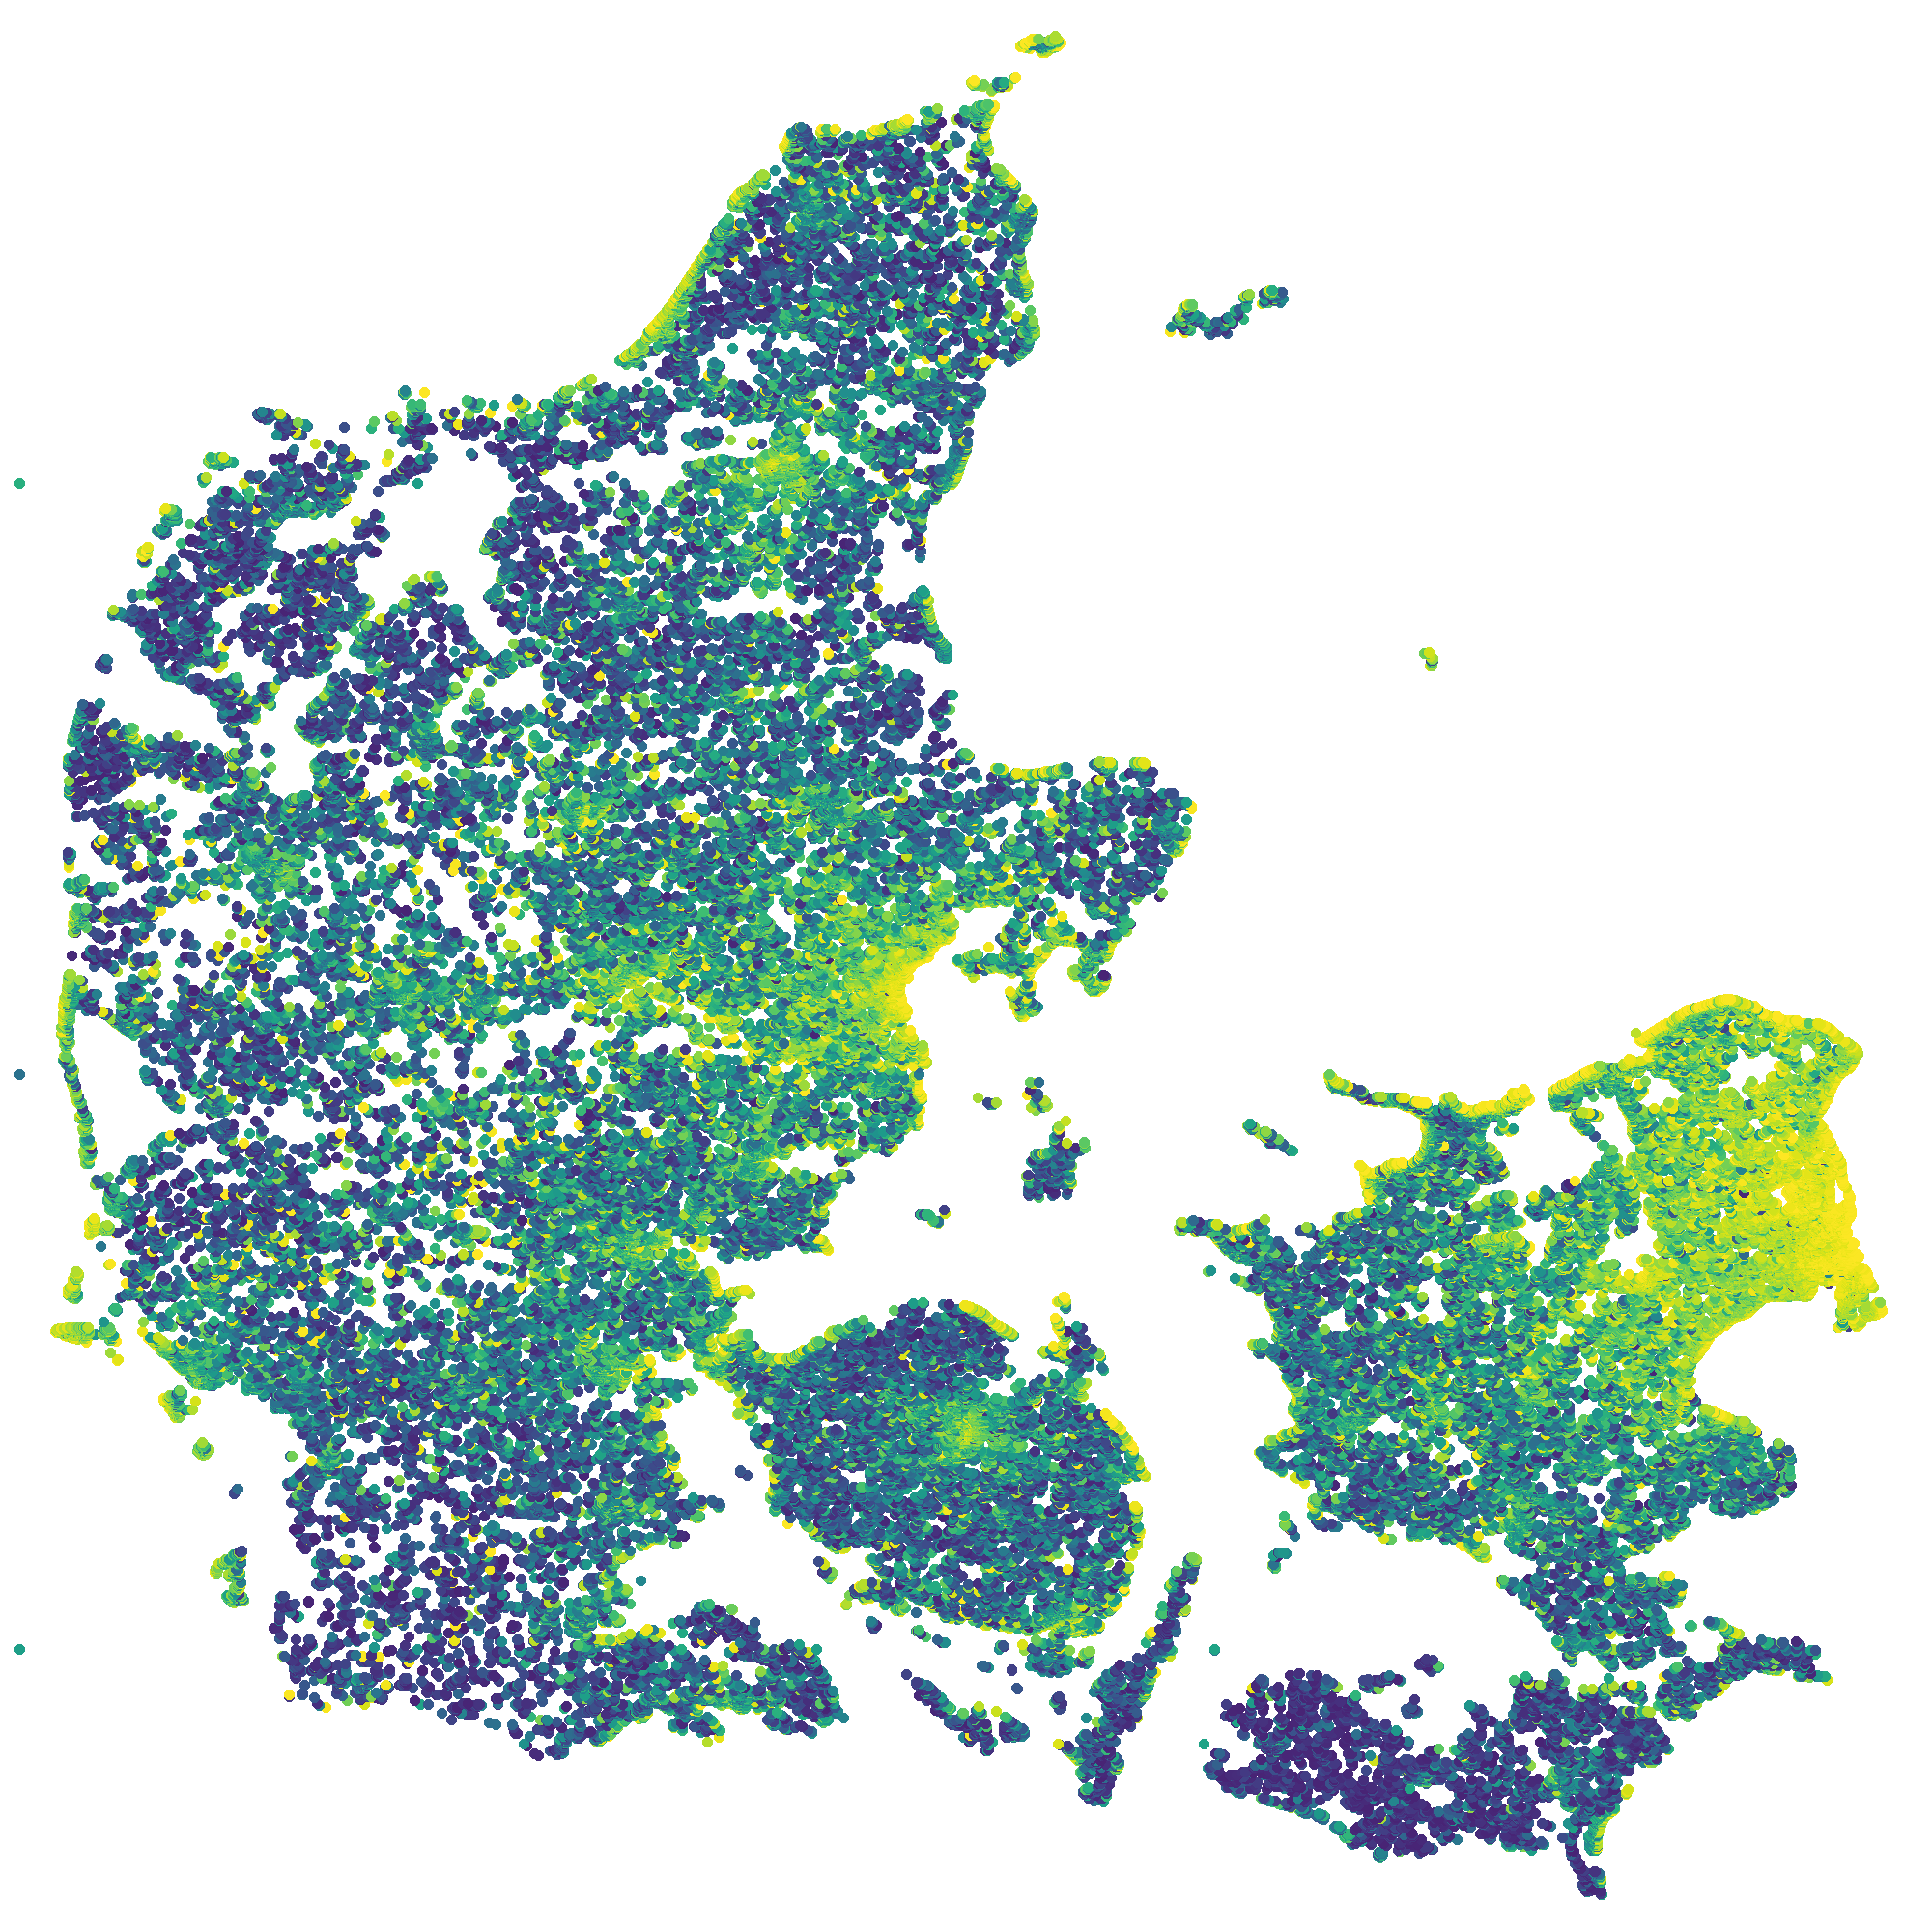
\includegraphics[draft=false, width=0.4\textwidth]{figures/housing/Denmark_Overview_SqmPrice.png}\hfil
  \subfloat[\label{fig:h:geo_overview_sales_price}]{\,}
  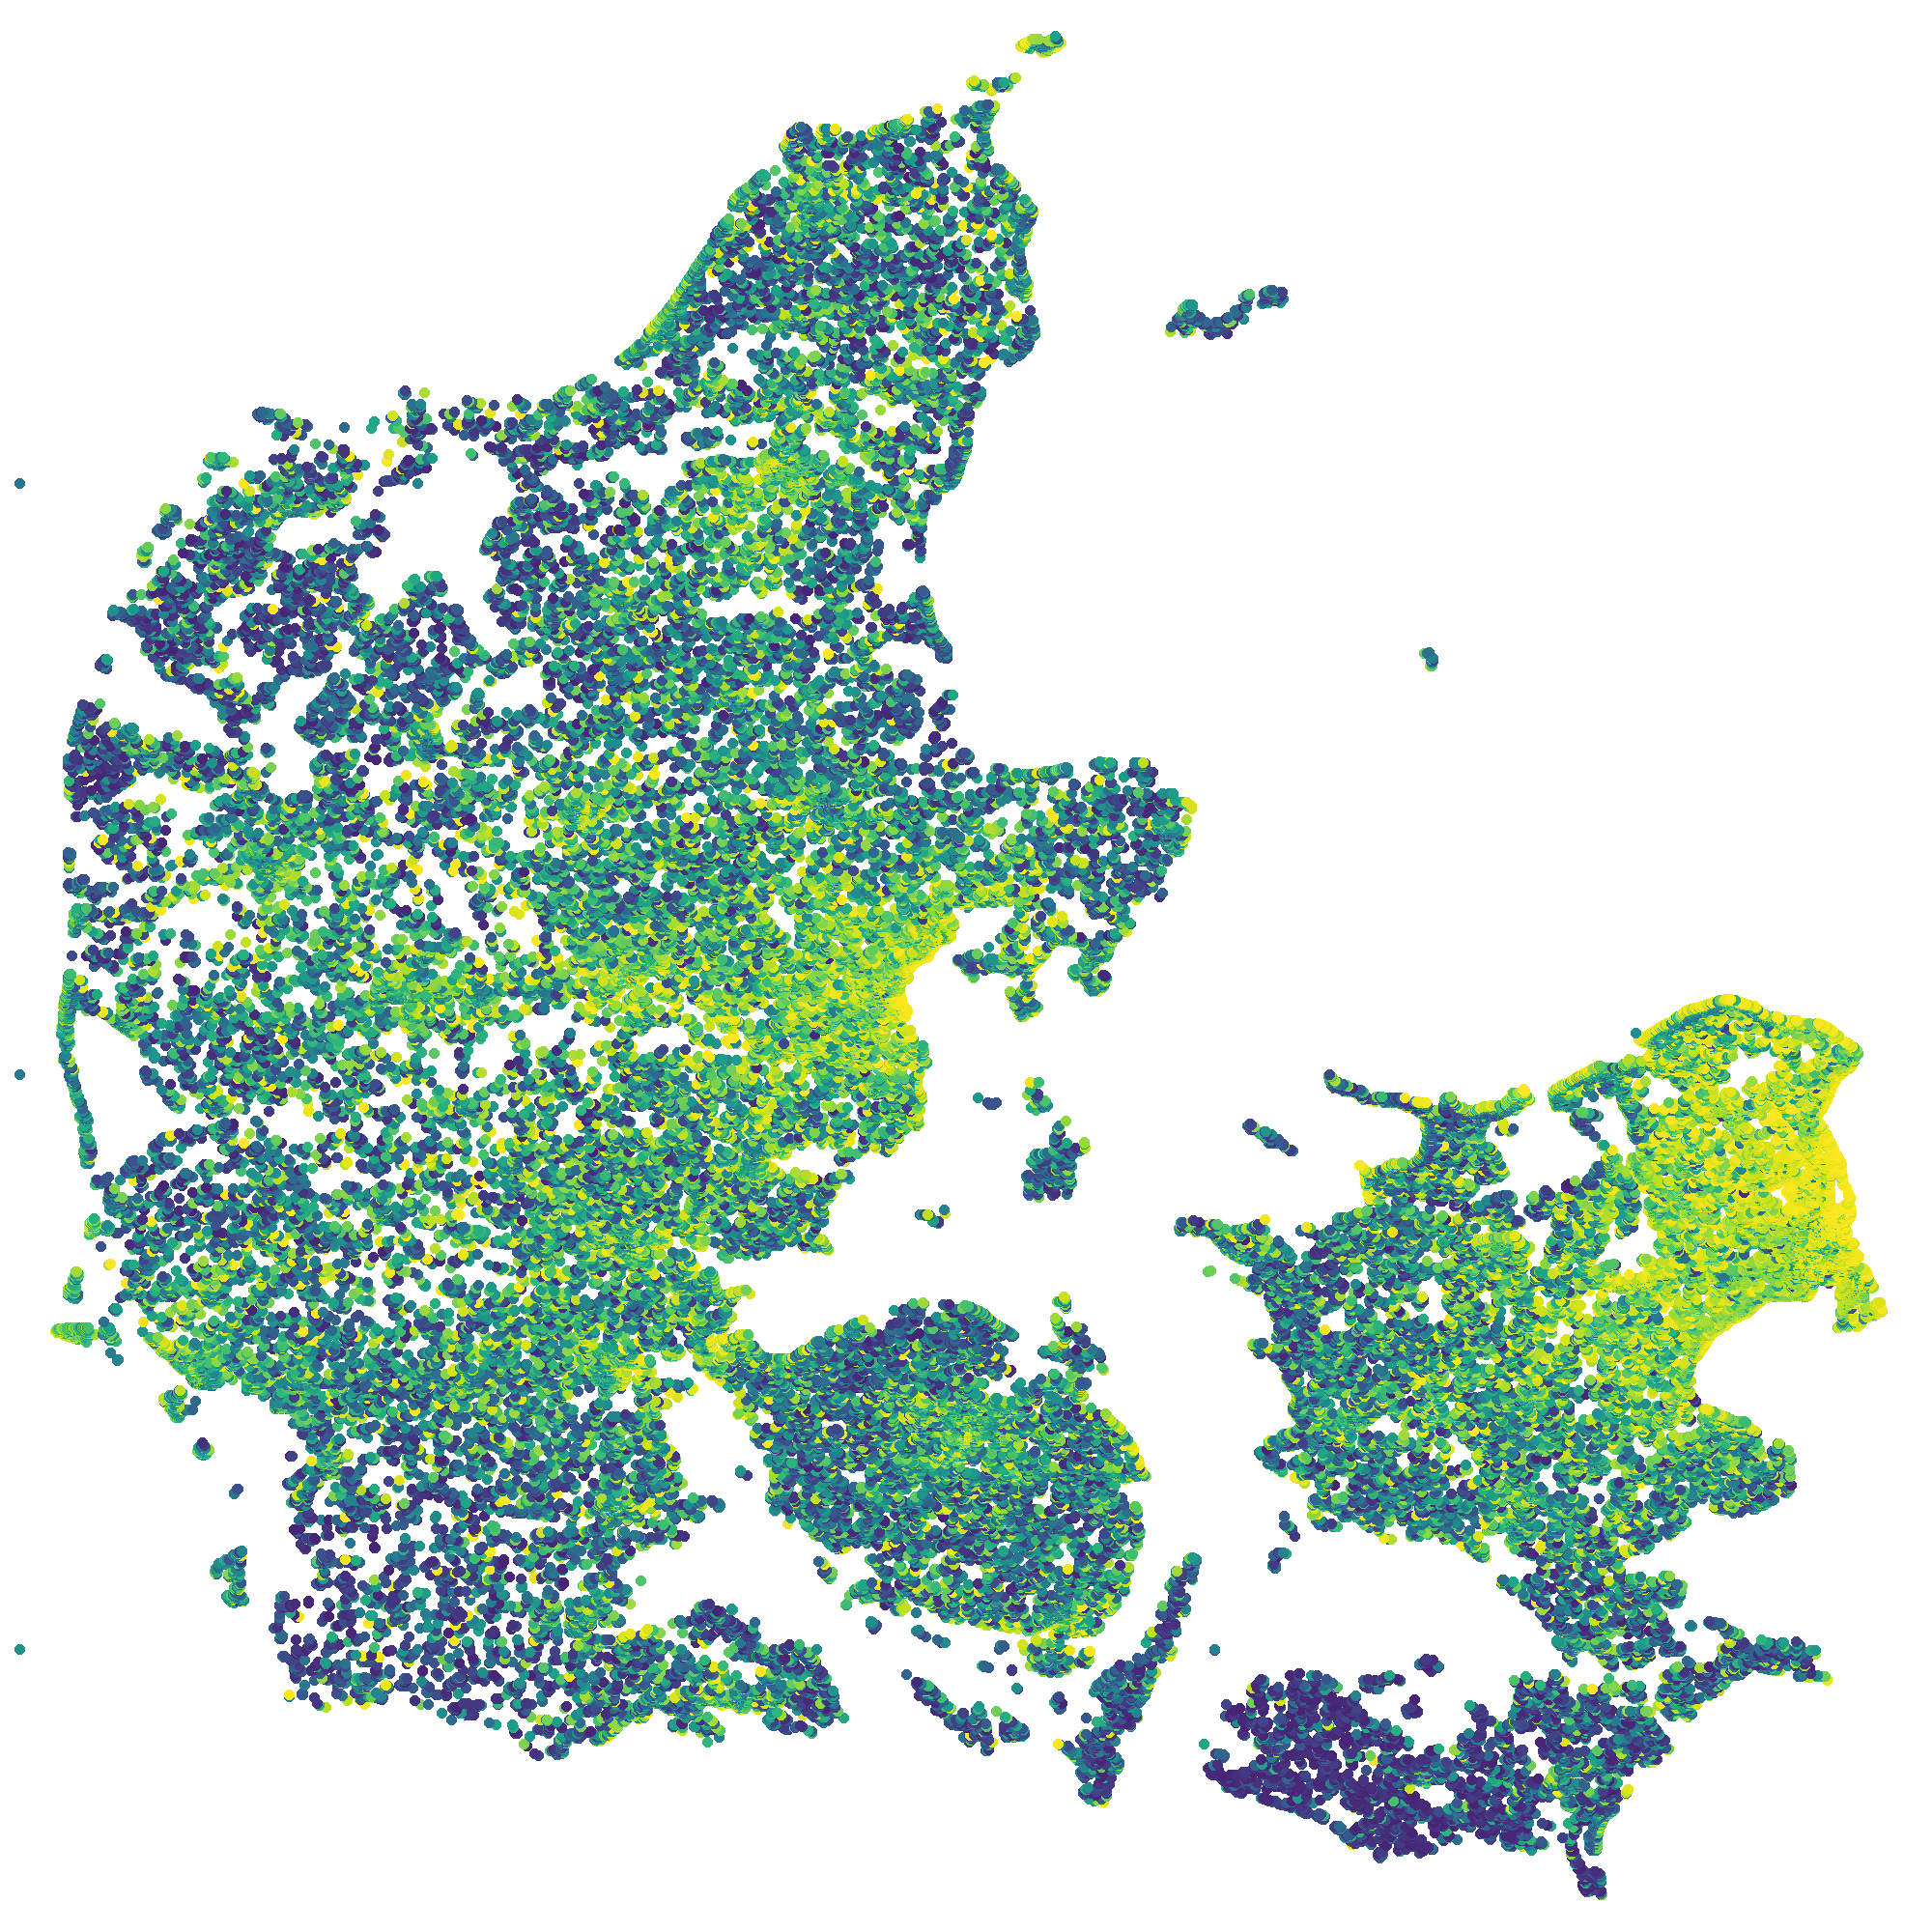
\includegraphics[draft=false, width=0.4\textwidth]{figures/housing/Denmark_Overview_SalesPrice.png}
  \caption[Geographic Distribution of the Sold Residences]{Geographic distribution of the sold residences. 
           In subplot ~\protect\subref{fig:h:geo_overview_sqm_price} the sales are colored according to their square meter price and in subplot ~\protect\subref{fig:h:geo_overview_sales_price} according to the sales price. 
           }
  \label{fig:h:geo_overview}
  \vspace{\abovecaptionskip}
\end{figure*}

The most important of the features is the sales price, called \code{SalgsPris} in the dataset. Its distribution is shown in Figure~\ref{fig:h:price_overview_price}. This is a positively skewed distribution that shares visual similarities with a log-normal distribution. The mode\sidenote{Measured in millions DKK, \si{\Mkr}} of the all sales prices is \SI{1.1}{\Mkr} and the median is \SI{1.6}{\Mkr} The mean is \SI{2.0}{\Mkr} but this value is heavily influenced by a few very high values. 

\begin{figure}
  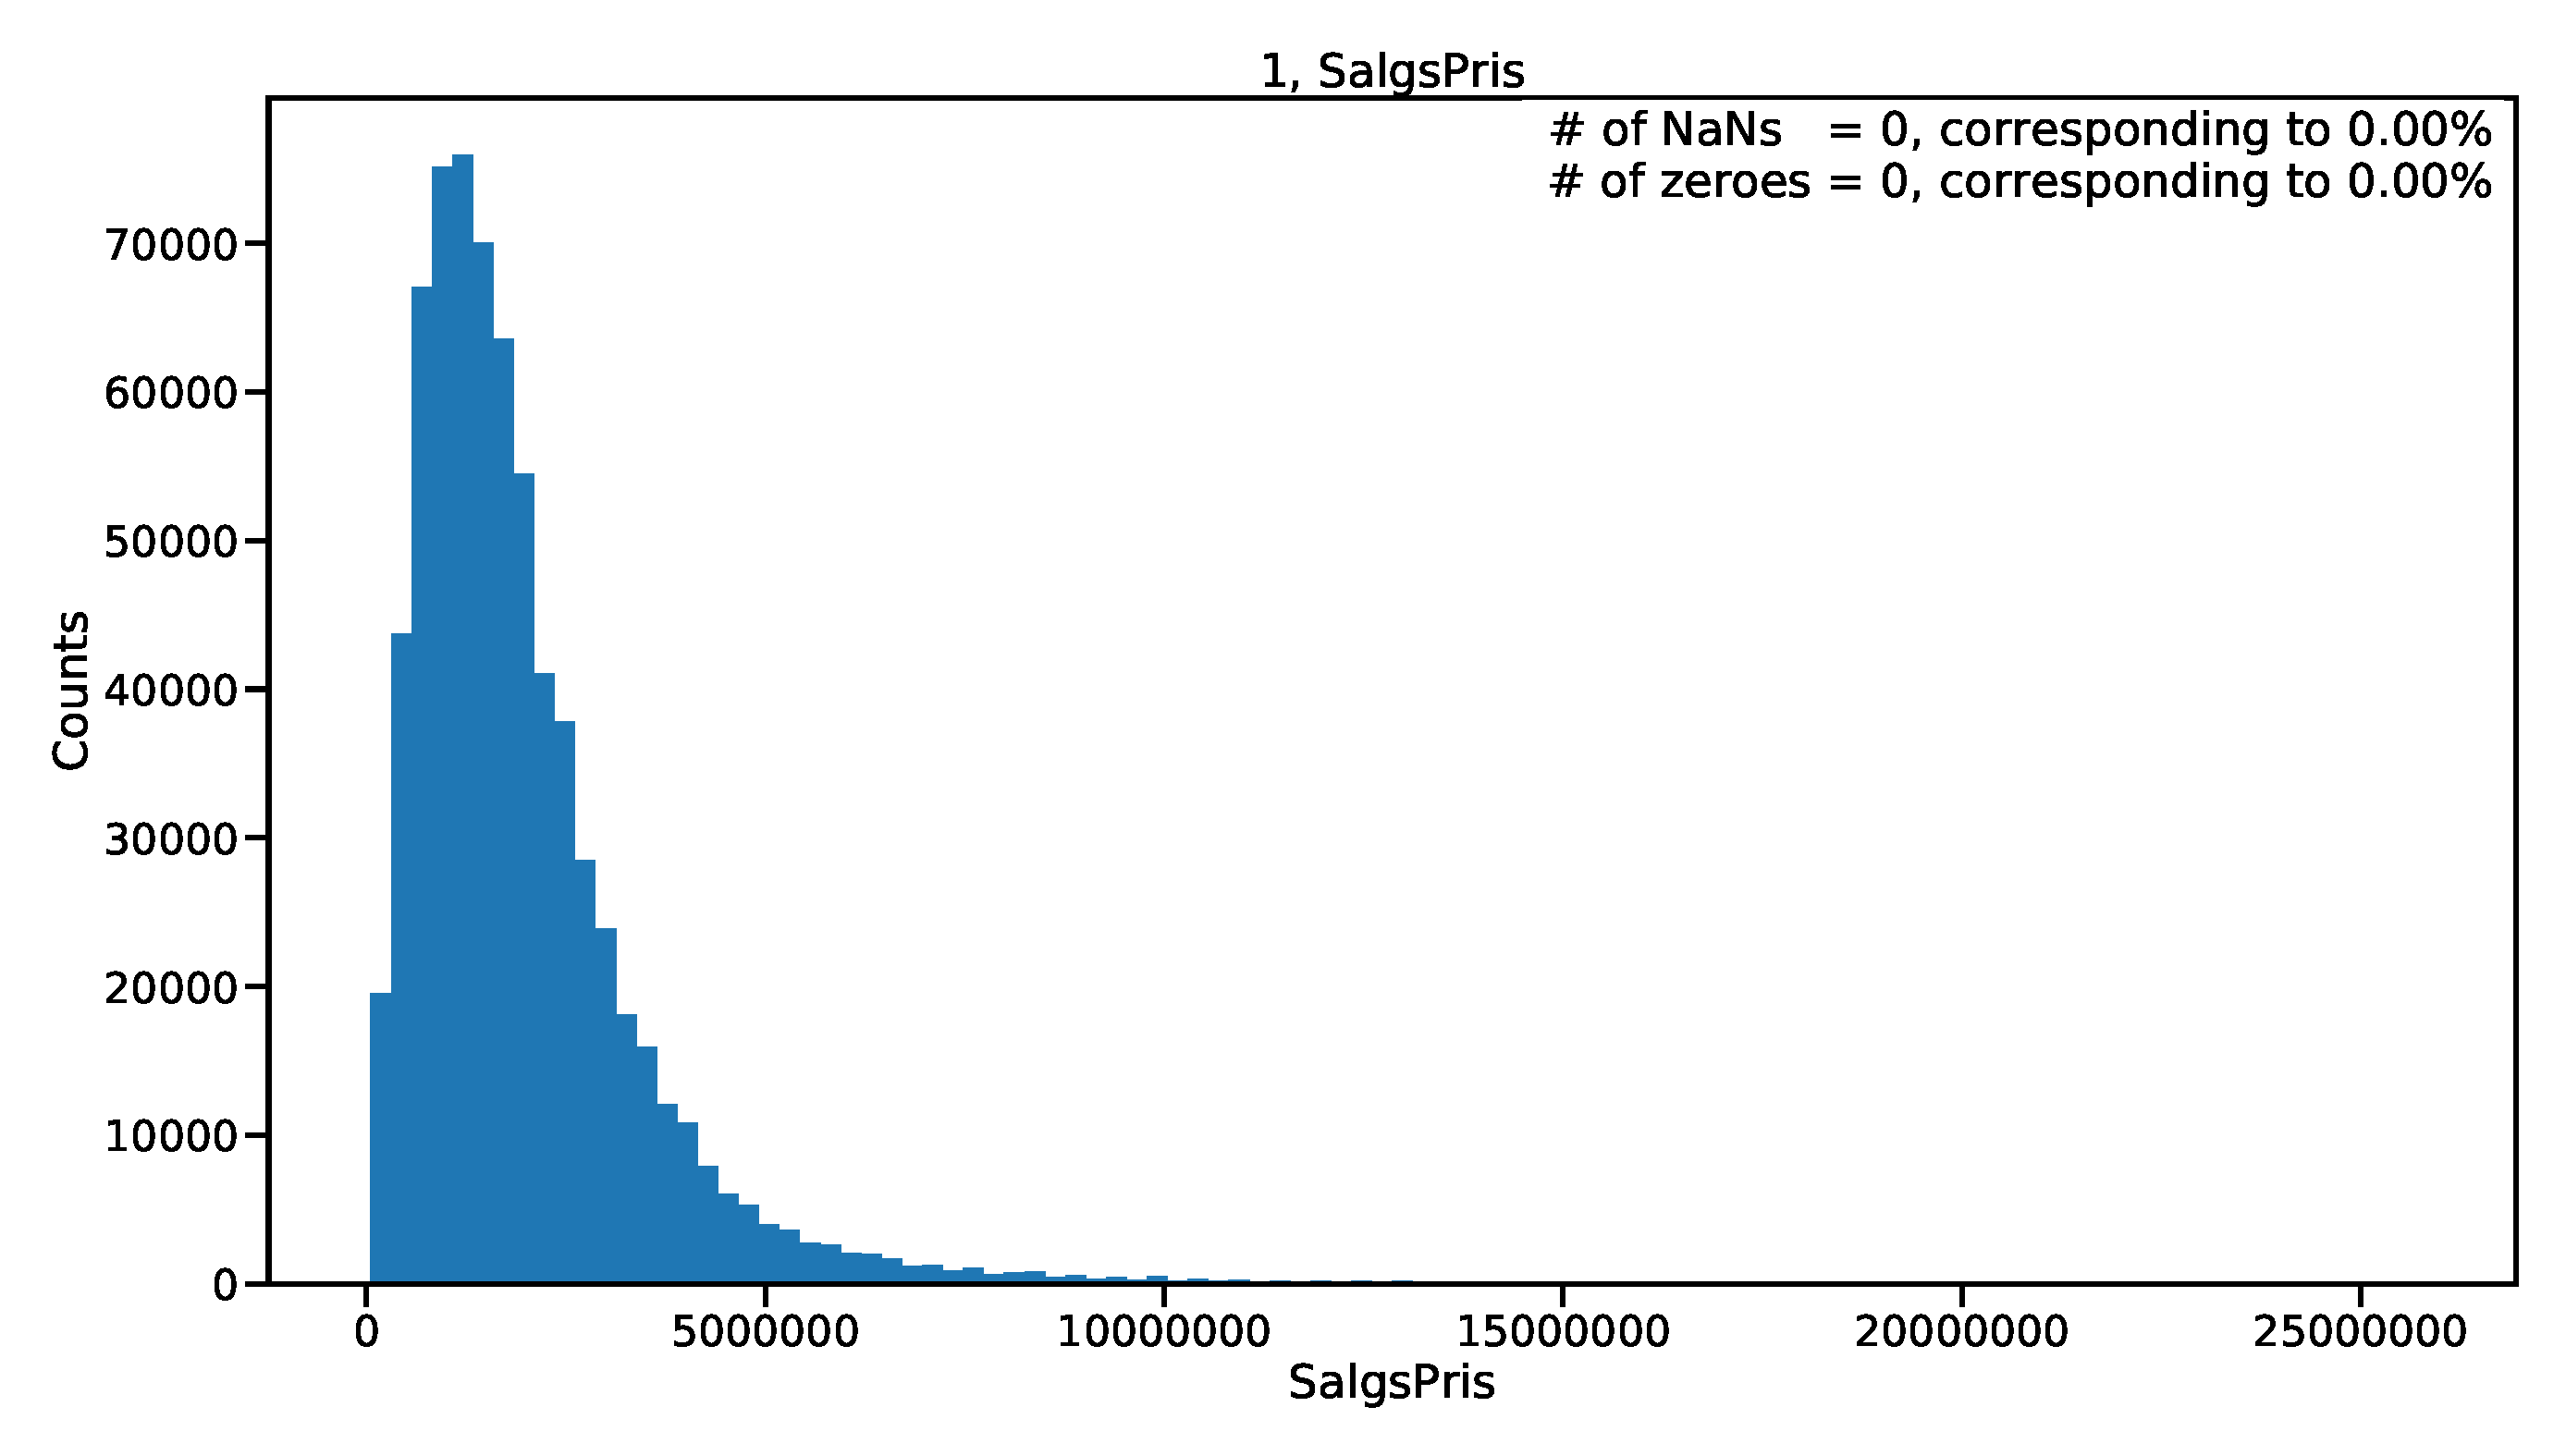
\includegraphics[width=0.98\textwidth, page=1, trim=15 15 15 15, clip]{figures/housing/overview_fig.pdf}
  \caption[Histogram of Prices of Houses and Apartments Sold in Denmark]
          {Histogram of prices of houses and apartments sold in Denmark.}
  \label{fig:h:price_overview_price}
\end{figure}

\subsection{Correlations}
\label{subsec:h:correlations_lin_mic}

Having shown the \num{1}D-distributions of all the different variables in the previous section, the next step would be to look at the correlations between the variables. Since there are \num{168} input variables, it is almost impossible to understand every inter-variable correlation, however, it is tried in Figure~\ref{fig:h:correlations_all_lin}. Here the correlation between all numerical variables that are not obviously related to other variables (like the GPS-coordinates that are in both latitude-longitude and ETRS89\sidenote{European Terrestrial Reference System \num{1989}.} format), and with the condition that it has to have one inter-variable correlation higher than $|\rho| > \SI{30}{\percent}$, are plotted as a $(86 \times 86)$-dimensional heatmap.

Even though inter-variable correlations are important in the exploratory data analysis (EDA) phase, what is more important is to get a better understanding of how the input variables correlate with the output variable; the sales price. This is shown in Figure~\ref{fig:h:corr_lin} for the variables where $\abs{\rho} > \SI{10}{\percent}$. It is the previous property evaluation, \code{EjdVurdering_EjendomsVaerdi} that is correlated the most with the sales price, which does not come as any huge surprise. Other positively correlated variables are the cost of ownership\sidenote{This a great example of the fact that correlation does not imply causation}, area, number of bathrooms, its longitude, and distance to nearest wind mill. In the other end, the local income tax, \code{Kommune_SkatteProcent}, is the variable that is the most negatively correlated to the sales price, followed by the geographical variables related to province, municipality, and postcode.

\begin{figure*}
  \centerfloat
  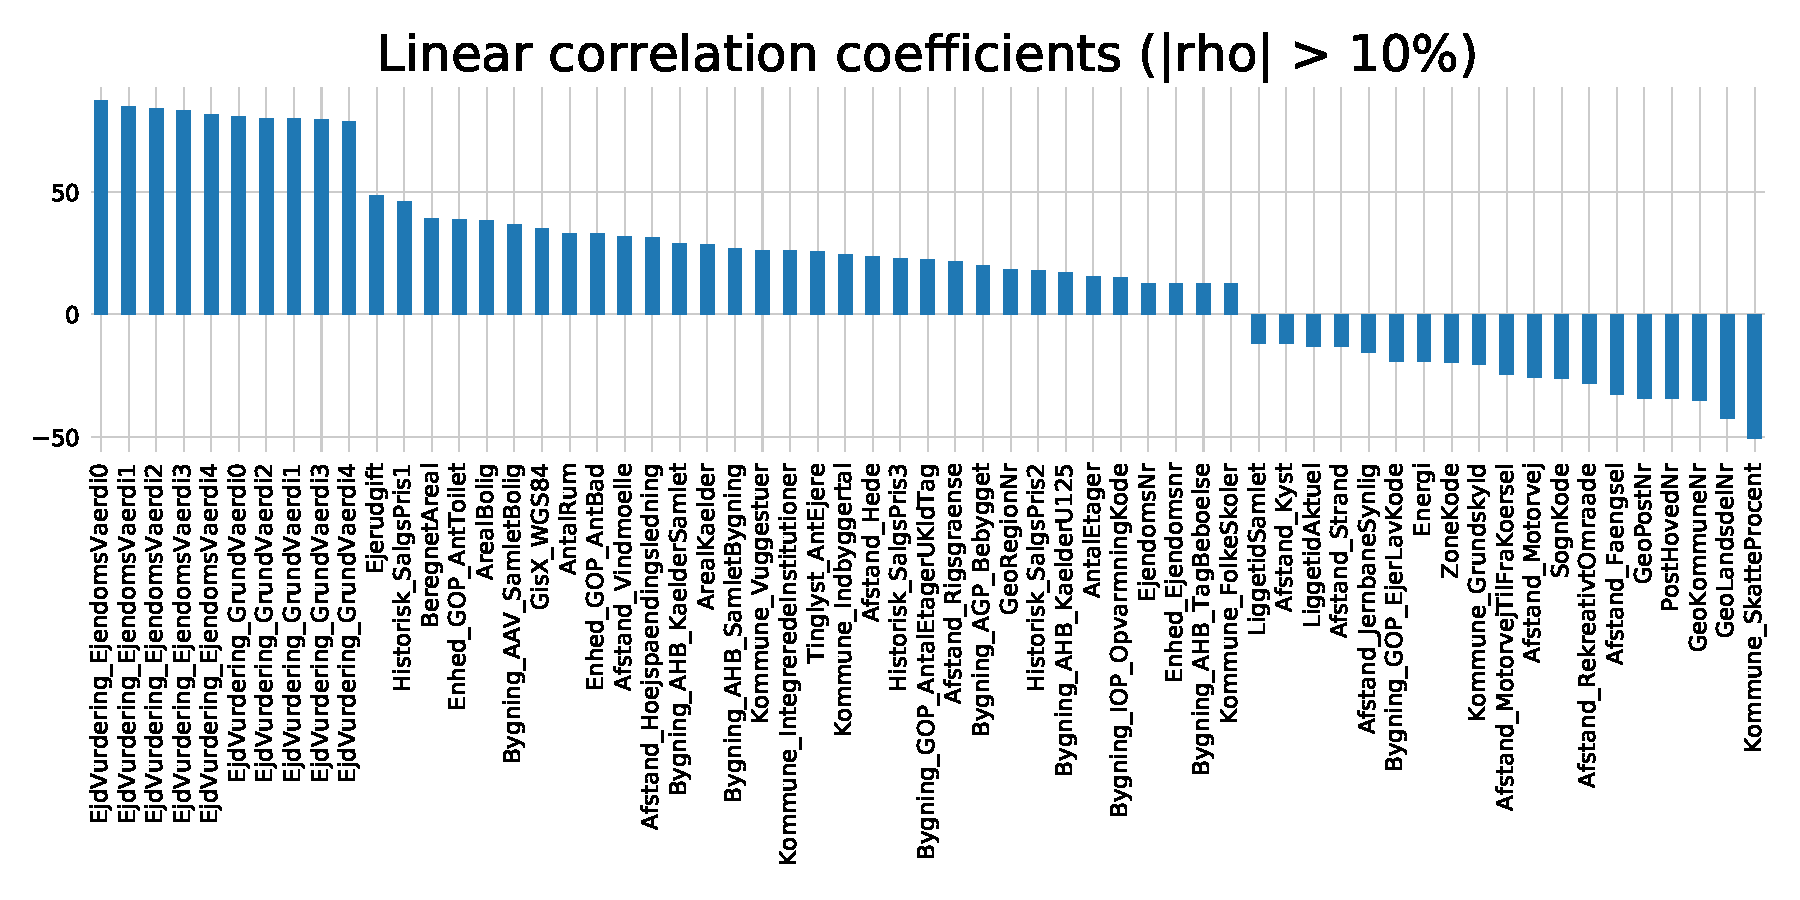
\includegraphics[width=0.99\textwidth, trim=20 10 0 40, clip]{figures/housing/lin_correlation.pdf}
  \caption[Linear Correlation Between Variables and Price]
          {Linear correlation between variables and price for variables where the correlation coefficient $\rho$ is $\abs{\rho} > \SI{10}{\percent}$.}
  \label{fig:h:corr_lin}
\end{figure*}

The correlation $\rho$ used above is the linear correlation which only captures linear relationships between variables. All modern machine learning algorithms, however, are also able to capture higher-order correlations and thus a higher-order correlation measure is needed. The maximal information coefficient (MIC), which is a value between \num{0} and \num{1}, is such a nonlinear measure. It finds correlation based on the intuition that if two variables are correlated, it should be possible to split the data up into smaller grids where, if they are correlated, the grid that contain points should contain many points and the rest of the grids should be (relatively) empty \autocite{reshefDetectingNovelAssociations2011}. This is in comparison to two uncorrelated variables which would simply display noisy behavior and only have few grids with many points in. \citet{albanesePracticalToolMaximal2018a} extended on this idea and developed the computationally efficient algorithm called MICtools which computes the estimator for MIC: $\mathrm{MIC}_e$. An example of this nonlinear correlation is seen in Figure~\ref{fig:h:MIC_example_small}. Here the relationship between the normal linear correlation $\rho$ and $\mathrm{MIC}_e$ are shown for four synthetic datasets. Notice that $\mathrm{MIC}_e$ does it particularly well for the sine wave, and decent for the line and parabola, but only slightly captures the relationship for the exponential growth. The influence of noise on $\rho$ and $\mathrm{MIC}_e$ can be see in Figure~\ref{fig:h:MIC_example}. 

\begin{figure}
  \centerfloat
  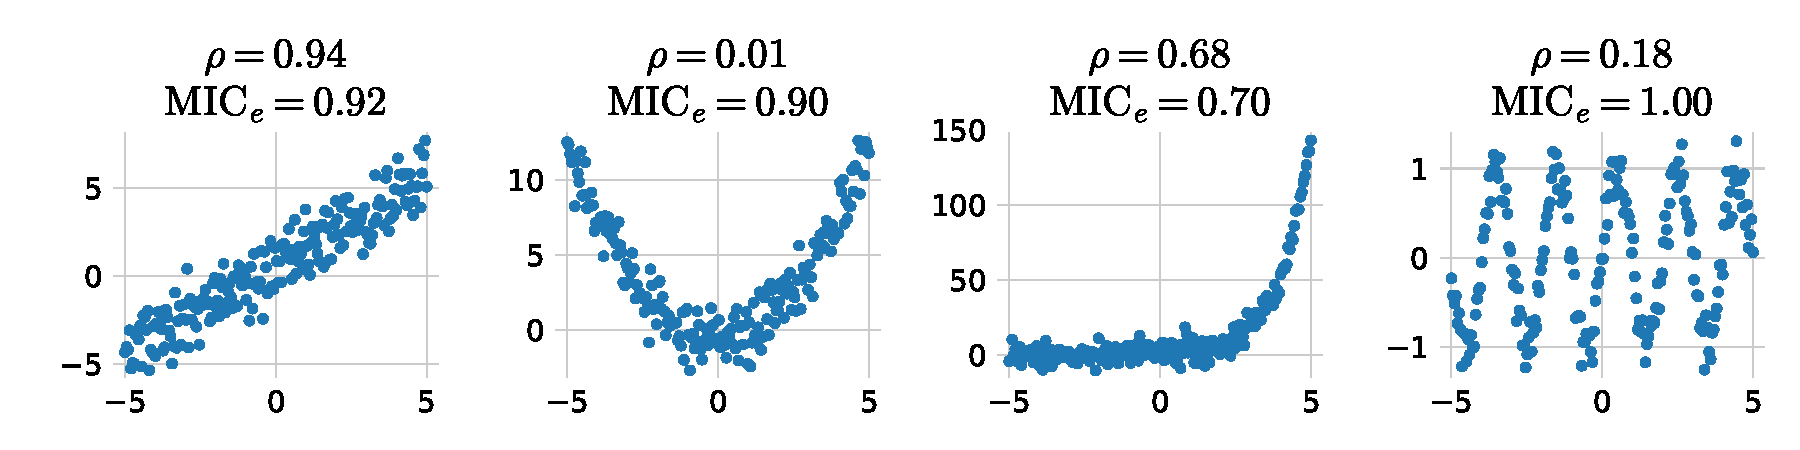
\includegraphics[width=0.99\textwidth, trim=10 10 10 10, clip]{figures/housing/MIC_test_small.pdf}
  \caption[Comparison of the Linear Correlation $\rho$ and the Nonlinear MIC]
          {Comparison of the linear correlation $\rho$ and the nonlinear MIC for a straight line, a parabola, an exponential, and a sine wave, all with noise added. See also Figure~\ref{fig:h:MIC_example}.}
  \label{fig:h:MIC_example_small}
\end{figure}

Using $\mathrm{MIC}_e$ as the correlation measure between the numerical variables and the sales prices, the variables with a $\mathrm{MIC}_e$-score higher than \SI{10}{\percent} are shown in Figure~\ref{fig:h:corr_MIC}. Again, the previous property evaluations are the most correlated features to the sales price followed by the parish code, \code{SogneKode}. In general the geographical variables score high here with also the post code, municipality number, and longitude. 

\begin{figure*}
  \centerfloat
  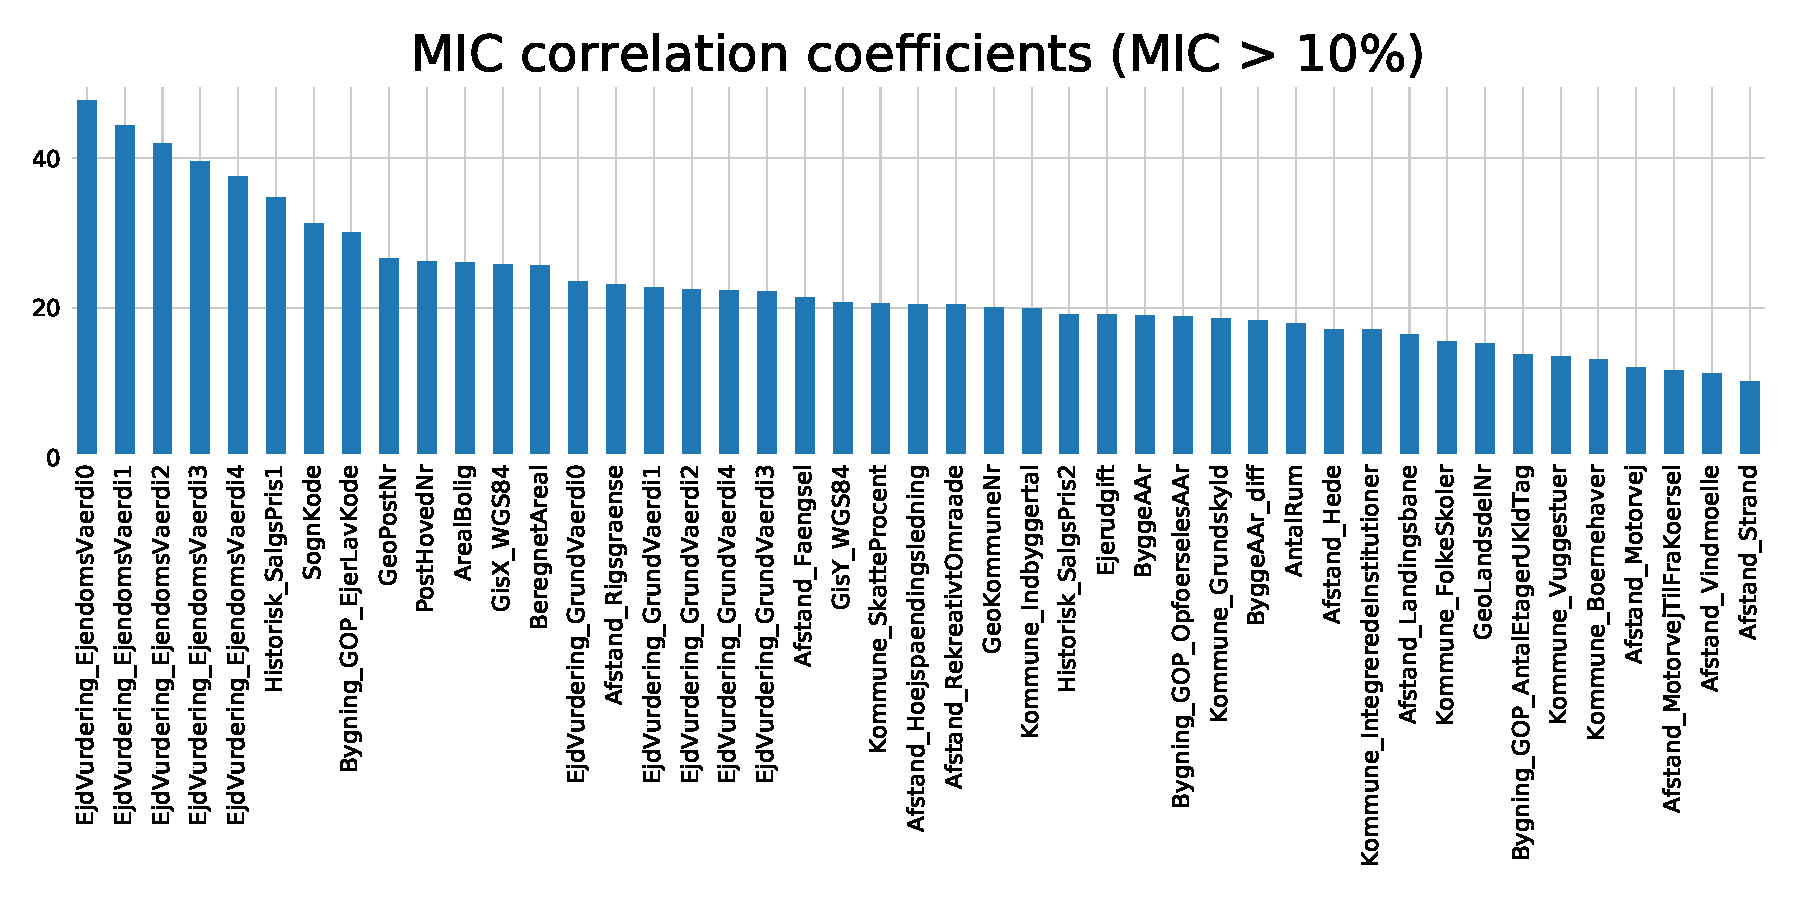
\includegraphics[width=0.99\textwidth, trim=10 10 0 40, clip]{figures/housing/MIC_plot.pdf}
  \caption[Nonlinear Correlation Between Variables and Price]
          {Nonlinear correlation between variables and price using Maximal Information Coefficient (MIC) for variables where $\text{MIC}>10\%$.}
  \label{fig:h:corr_MIC}
\end{figure*}

\subsection{Validity of Input Variables}

The fact that some of the variables contains considerable amount of invalid values, NANs, requires this to be taken into account before any further analysis. The validity, defined as the percentage of valid observations, of every variable is shown in Figure~\ref{fig:h:nans}. Here the \num{168} variables variables are grouped together into \num{25} variables where each group share the same validity. An example of this are all of the \num{16} different distance-variables\sidenote{Distance to: prison, heath, high-voltage transmission line, industri, visible railroad, church, churchyard, coast, landing strip, motorway, access to motorway, recreational area, border, sports centre, beach, and windmill.}. We see that most of the variables have validities around more than 
\SI{85}{\percent}, however, a few of the variables, especially information about the building, \code{BygningsInfo}, have validities less than \SI{20}{\percent}. 

% \sidenote{Distance to: Fængsel, Hede, Højspaendingsledning, Industri, JernbaneSynlig, Kirke, Kirkegård, Kyst, Landingsbane, Motorvej, MotorvejTilFraKørsel, RekreativtOmråde, Rigsgrænse, Sportsanlæg, Strand, Vindmølle}

\begin{figure*}
  \centerfloat
  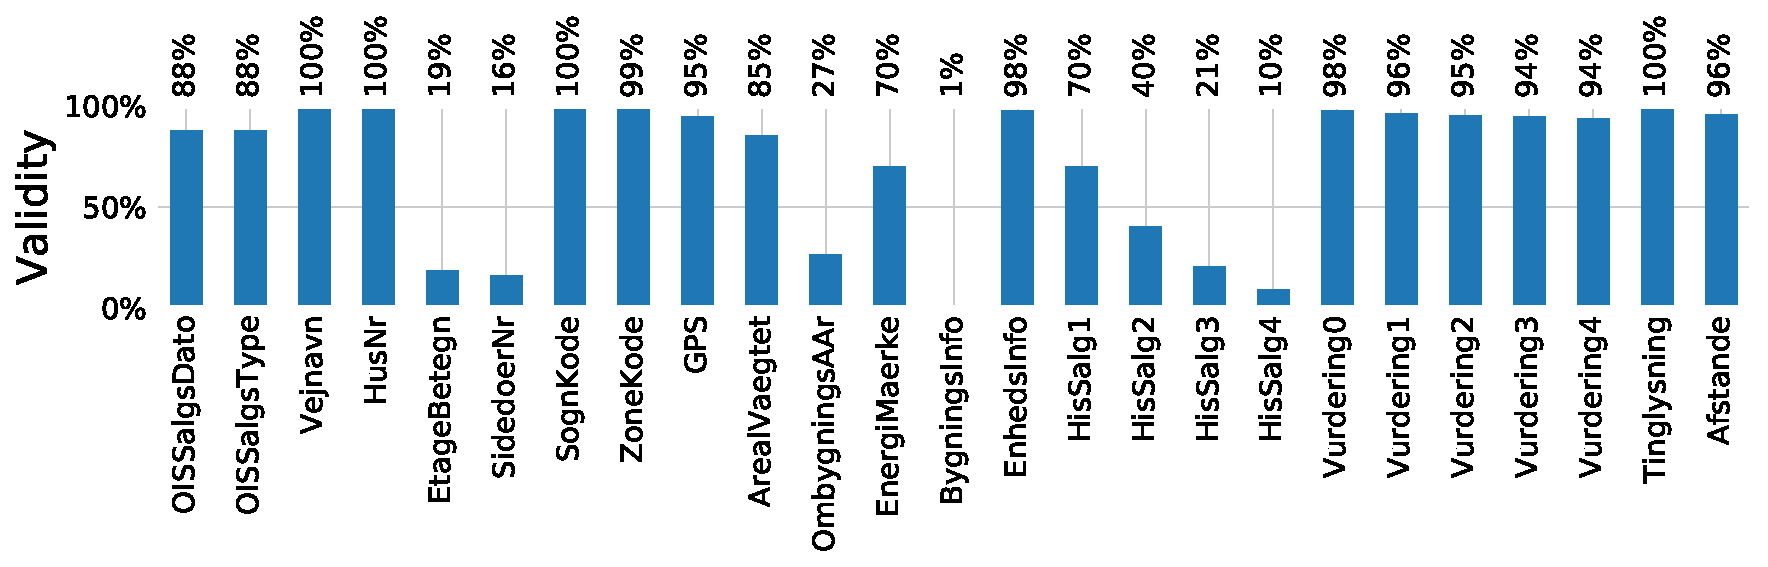
\includegraphics[width=0.9\textwidth, trim=0 0 0 0, clip]{figures/housing/missing_bar.pdf}
  \caption[Validity of Input Features]
          {Percentage of valid counts for each variable grouped together in categories.}
  \label{fig:h:nans}
\end{figure*}

To see how closely related the different validity groups are, one can look at the dendrogram in Figure~\ref{fig:h:nans_dendrogram}. The dendrogram is based on a hierarchical clustering algorithm \citep{virtanenSciPyFundamentalAlgorithms2019} where the different groups are clustered according to the linear correlation of their validity. This diagram is supposed to be read in a top-down approach, where it can be see that the name of the street, \code{Vejnavn}, and the number of the residence, \code{HusNr}, correlate a lot and are thus clustered very early. The year of the last time the residence was rebuilt or greatly modified, \code{OmbygningsAAr}, does not correlate strongly with any of the other variables and is thus the last variable to be clustered together. 

\begin{figure}
  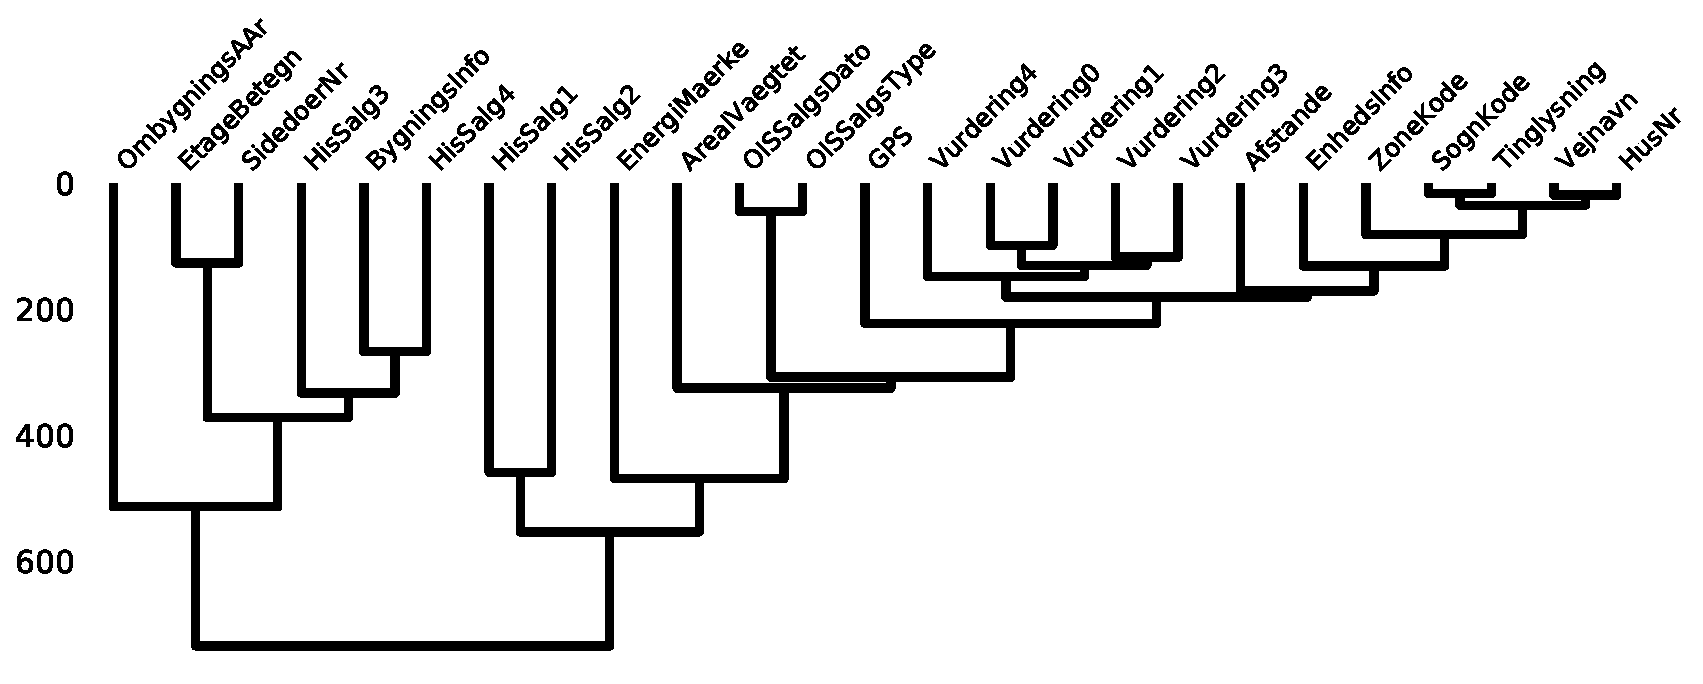
\includegraphics[width=0.98\textwidth, trim=35 10 0 10, clip]{figures/housing/missing_dendrogram.pdf}
  \caption[Validity Dendrogram]
          {Validity Dendrogram based on hierarchical clustering of the linear correlation of validity for the housing price variables clustered together.}
  \label{fig:h:nans_dendrogram}
\end{figure}

To see a heatmap of the validity inter-variable correlations, see Figure~\ref{fig:h:nans_heatmap}. 

\subsection{Cuts}
Given the 1D input variable distributions and their validity, we apply some very basic cuts before any further analysis. These cuts are seen in Table \ref{tab:h:initial_cuts}. Sales type, \code{OISSalgsType}, is a OIS\sidenote{OIS is short for \q{Den Offentlige Informationsserver}, the Danish public information server, and it collects information about Danish residences \autocite{oisWwwOISDk}.} code which describes what type of sale it is: when it is \num{1} it is considered a normal sale, compared to e.g. forced sales. These cuts are seen as the minimum requirements for what constitutes a curated dataset with no obvious outliers. The reason why the time requirement is applied is to reduce the effect of the financial crisis to creep into the model. 

\begin{table}[h]
  \begin{tabular}{@{}llcr@{}}
  % \toprule
               & Description                                          & Remaining & Removed \\ 
  \midrule
  Area         & \SI{20}{\meter\squared} $\leq$ Area $\leq$ \SI{500}{\meter\squared} & \num{689140}              & \num{23666}     \\
  Price        & \SI{0.1}{\Mkr} $\leq$ Price $\leq$ \SI{100}{\Mkr}                   & \num{687546}              & \num[group-minimum-digits=3]{1594}      \\
  Type         & Has sales type \num{1}                                              & \num{605415}              & \num{82131}     \\
  GPS          & Has valid GPS coordinates                                           & \num{578860}              & \num{26555}     \\
  Private      & Only non-business sales                                             & \num{549140}              & \num{29720}     \\
  Time         & Sold in \num{2009} or later                                         & \num{520548}              & \num{28592}     \\
  \bottomrule
  \end{tabular}
  \vspace{\abovecaptionskip}
  \caption[Basic Cuts]{Overview of the basic cuts which define the minimum information needed to predict the price of a sale.}
  \label{tab:h:initial_cuts}
\end{table}

\section{Feature Augmentation}
\label{sec:h:feature_augmentation}

\begin{margintable}
  % \begin{tabular}{llr}
  \begin{tabular*}{\textwidth}{l @{\extracolsep{\fill}} lr}
  % \toprule
  String & Explanation  & Code \\ \midrule
  NAN    & No side door & \num{0}    \\
  TH, TV & Right, left  & \num{11}   \\
  MF     & Center       & \num{12}   \\
  --     & The rest     & \num{15} 
  \end{tabular*}
  \vspace{1mm}
  \caption[Side Door Mapping.]{Side door mapping. If the side door string contains e.g. \q{TH} this gets the code \num{11}.}
  \label{tab:h:sidedoor_code}
  \vspace{3mm}
\end{margintable}


\begin{margintable}
  % \vspace{\abovecaptionskip}
  % \begin{tabular}{llr}
  \begin{tabular*}{\textwidth}{l @{\extracolsep{\fill}} lr}
  Contains   & Explanation  & Code \\ \midrule
  Vej        & Road       & \num{0}    \\
  Gade       & Street     & \num{1}    \\
  Alle, Allé & Avenue     & \num{2}    \\
  Boulevard  & Boulevard  & \num{3}    \\
  --         & The rest   & \num{-1}  
  \end{tabular*}
  \vspace{1mm}
  \caption[Street Mapping]{Street mapping. If the street name contains e.g. \q{Vej} this gets the code \num{0}.}
  \label{tab:h:road_code}
  \vspace{3mm}
\end{margintable}


Until now the analysis have dealt with different types of residences all together. From now on, the rest of the analysis will be applied on single-family houses and owner-occupied apartments independently. 

First invalid counts are dropped such that variables which contain more than \SI{10}{\percent} NANs are dropped, and duplicate rows are also removed. Then some manual features are added based on existing features. The day of the month, the month, and the year are extracted from the sales date and the sales date is also represented as the numbers of days since January \nth{1}, \num{2009}. From the number of the house, \code{HusNr}, the number is extracted along with a boolean flag indicating whether or not it includes a letter (eg. \q{27B}). The number of the side door, \code{SidedoerNr}, is formatted according to Table~\ref{tab:h:sidedoor_code} and the road name is according to  Table~\ref{tab:h:road_code}. The age of the house is added\sidenote{In addition to only having the year the house was was built.} and the amount of time (in years) since last major modification. The energy rating label, \code{EnergiMaerke}, is also converted from strings to values according to Table~\ref{tab:h:energy_code}.

Finally, some of the variables in the dataset are not suitable for machine learning or simply transformations of other variables. These are variables such as the ID, when the house was deleted at Boligsiden, or the cash price. They are dropped since we do not want the model to learn the price of the residence using these variables.

\subsection{Time-Dependent Price Index}

In addition to the manual data augmentation in \autoref{sec:h:feature_augmentation}, a time-dependent price index is also added. We make use of the open source package called Prophet made by \citet{taylorForecastingScale} at Facebook. It is based on a decomposable time series model \autocite{harveyEstimationProceduresStructural1990} with two\sidenote{In their paper, \citet{taylorForecastingScale} include a holiday component in their analysis as well which is not included in this project.} components; trend $g(t)$ and seasonality $s(t)$:
\begin{equation}
  y_\mathrm{Prophet}(t) = g(t) + s(t) + \epsilon_t,
\end{equation}
where $\epsilon_t$ is a normally distributed error term. \citet{taylorForecastingScale} fit this equation with a generalized additive model (GAM) \autocite{hastieGeneralizedAdditiveModels1987} which they argue has several practical advantages compared to ARIMA \sidenote{AutoRegressive Integrated Moving Average.} models which commonly used in economics \autocite{nla.cat-vn1067782}. 

We fit the Prophet model on the weekly median price pr. square meter (PPSM) up until (and including) \num{2017}. The results of the prophet model fitted on (owner-occupied) apartments are seen in Figure~\ref{fig:h:prophet_forecast} and Figure~\ref{fig:h:prophet_trends}. In Figure~\ref{fig:h:prophet_forecast} the weakly median price pr. square meter for apartments are shown as black dots with the fitted Prophet model shown in blue. The $1\sigma$ uncertainty intervals are shown as the transparent blue band. The Prophet model not only allows predicting previous and future PPSMs, it also return the uncertainty of this prediction. The future predictions for the PPSM are the values after 2018. The trend and seasonality of the model are shown in Figure~\ref{fig:h:prophet_trends} where the top plot is the overall trend $g(t)$ and the bottom plot is the seasonality $s(t)$. Whereas the trend just continues to rise, the seasonality shows that residences are generally sold for a higher price in the Summer months compared to the Winter months. 
The Prophet model plots for one-family houses are shown in Figure~\ref{fig:h:prophet_forecast_villa} and \ref{fig:h:prophet_trends_villa}. 

\begin{figure}
  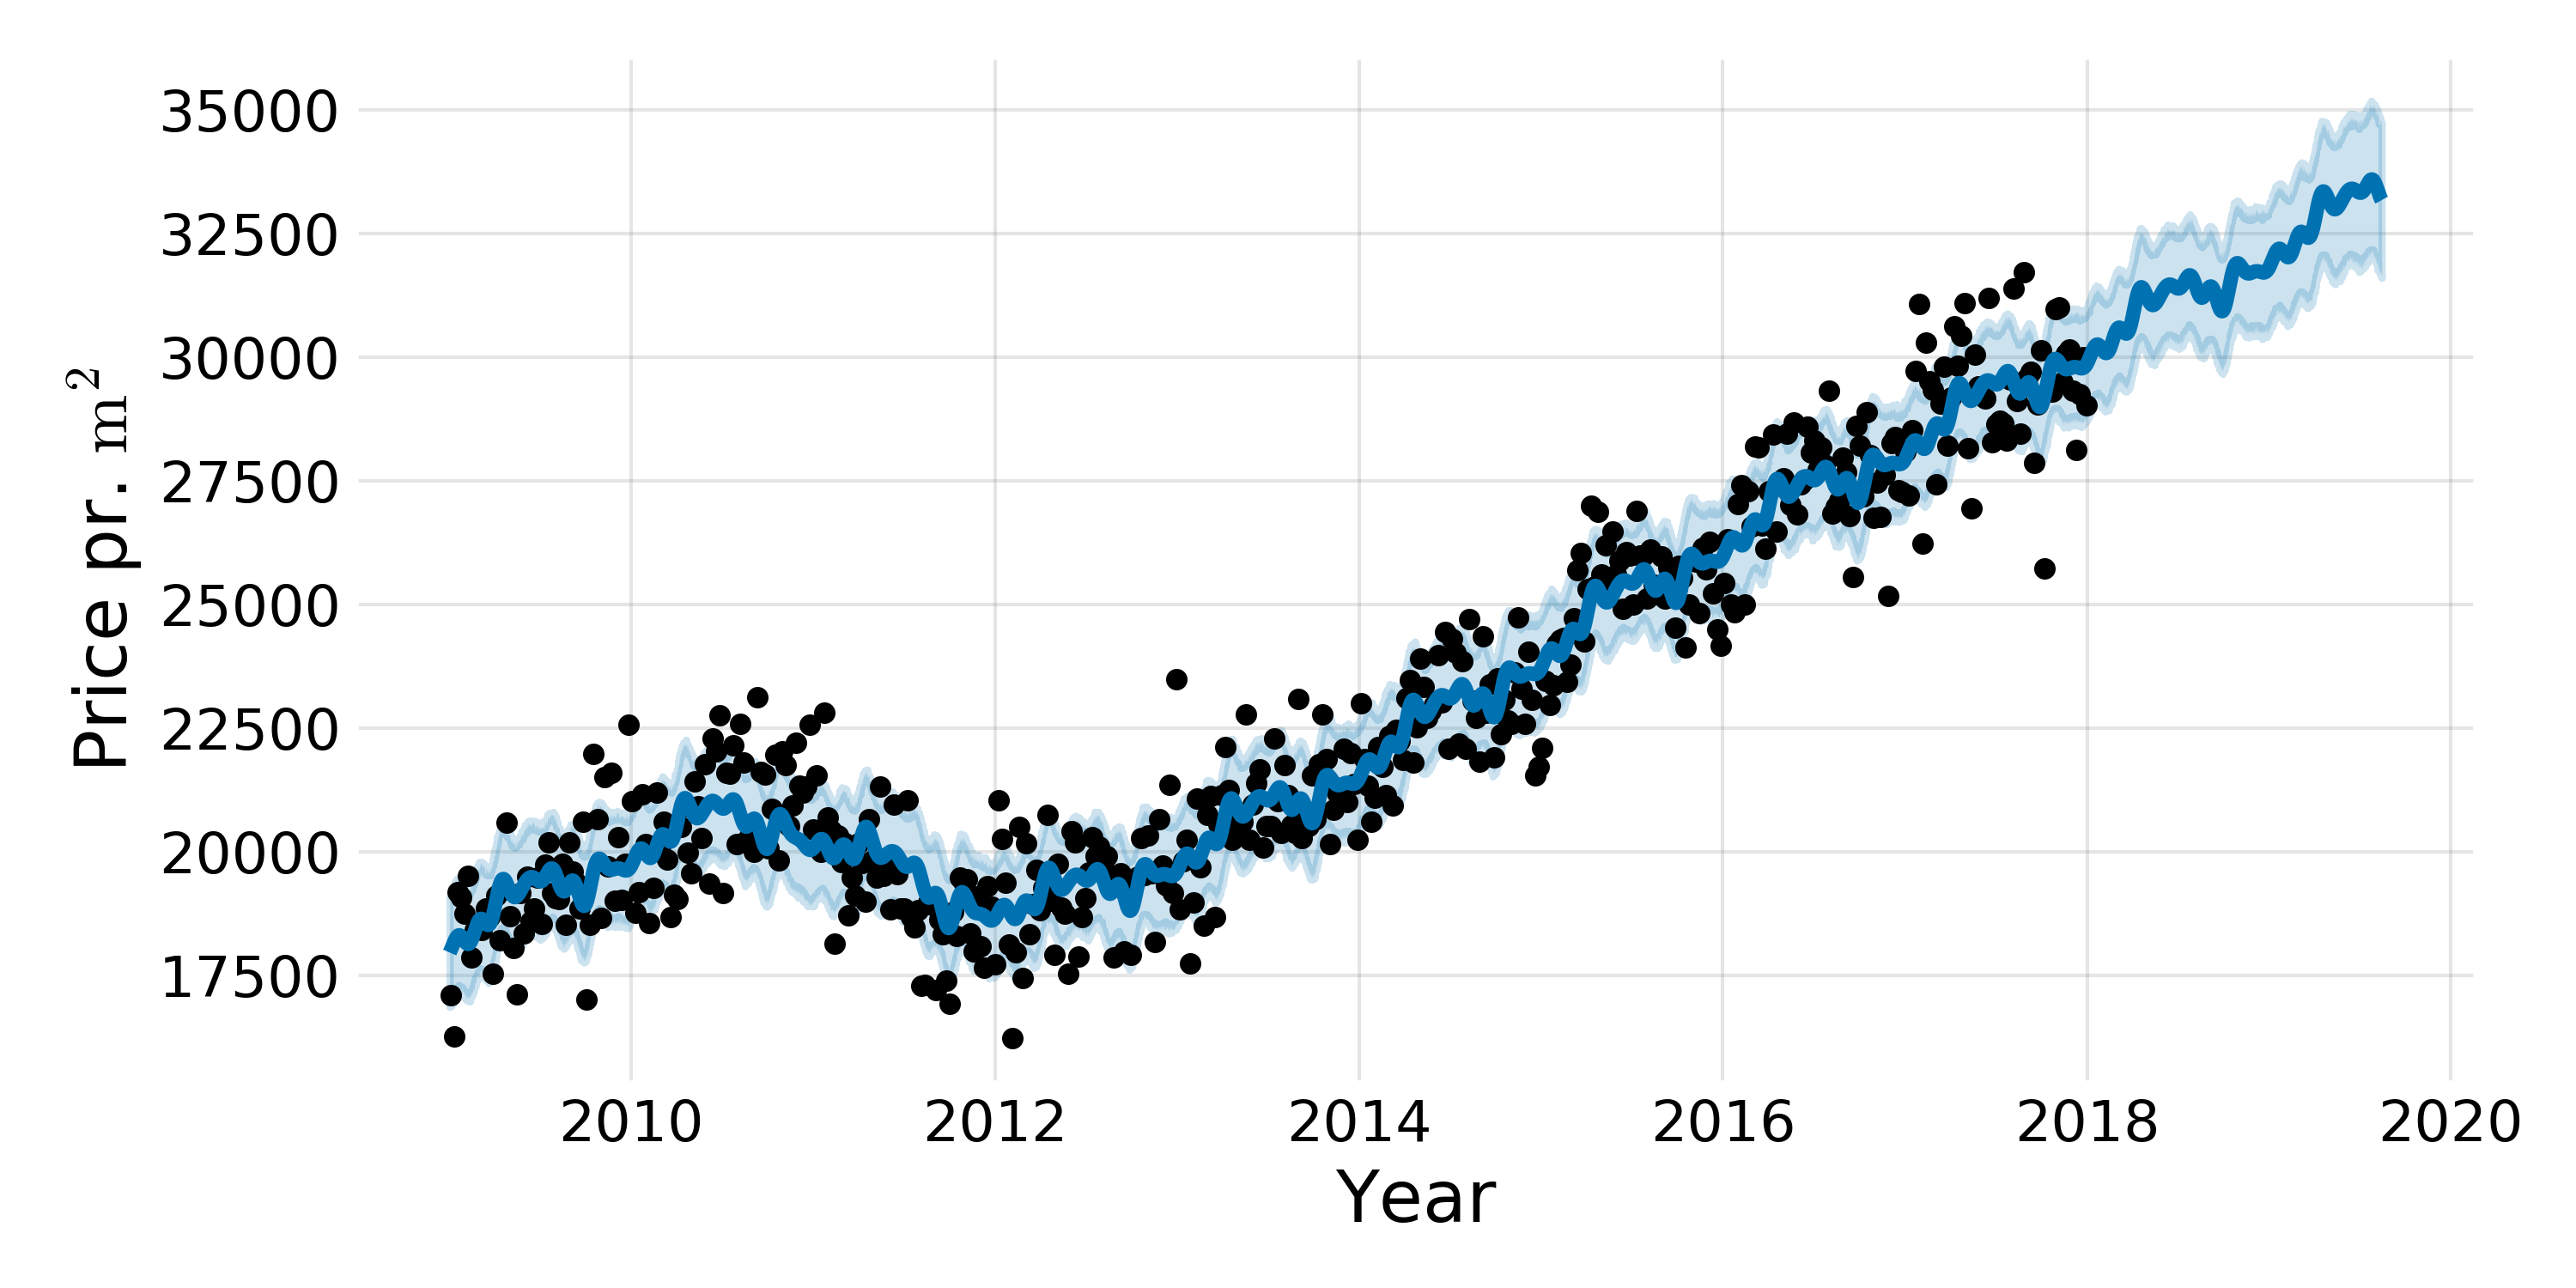
\includegraphics[draft=false, width=0.9\textwidth, trim=15 15 15 15, clip]{figures/housing/Ejerlejlighed_v18_cut_all_Ncols_all_prophet_forecast.png}
  \caption[Prophet Forecast for Apartments]
          {The predictions of the Facebook Prophet model trained on square meter prices for owner-occupied apartments sold before January 1st, 2018. The data is down-sampled to weekly bins where the median of each week is used as in input to the Prophet model, shown seen as black dots in the figure. The \textcolor{blue}{model's forecasts} for 2018 and 2019 are shown in blue with a light blue \textcolor{light-blue}{error band} showing the $1\sigma$ confidence interval.
          }
  \label{fig:h:prophet_forecast}
\end{figure}

\begin{figure}
  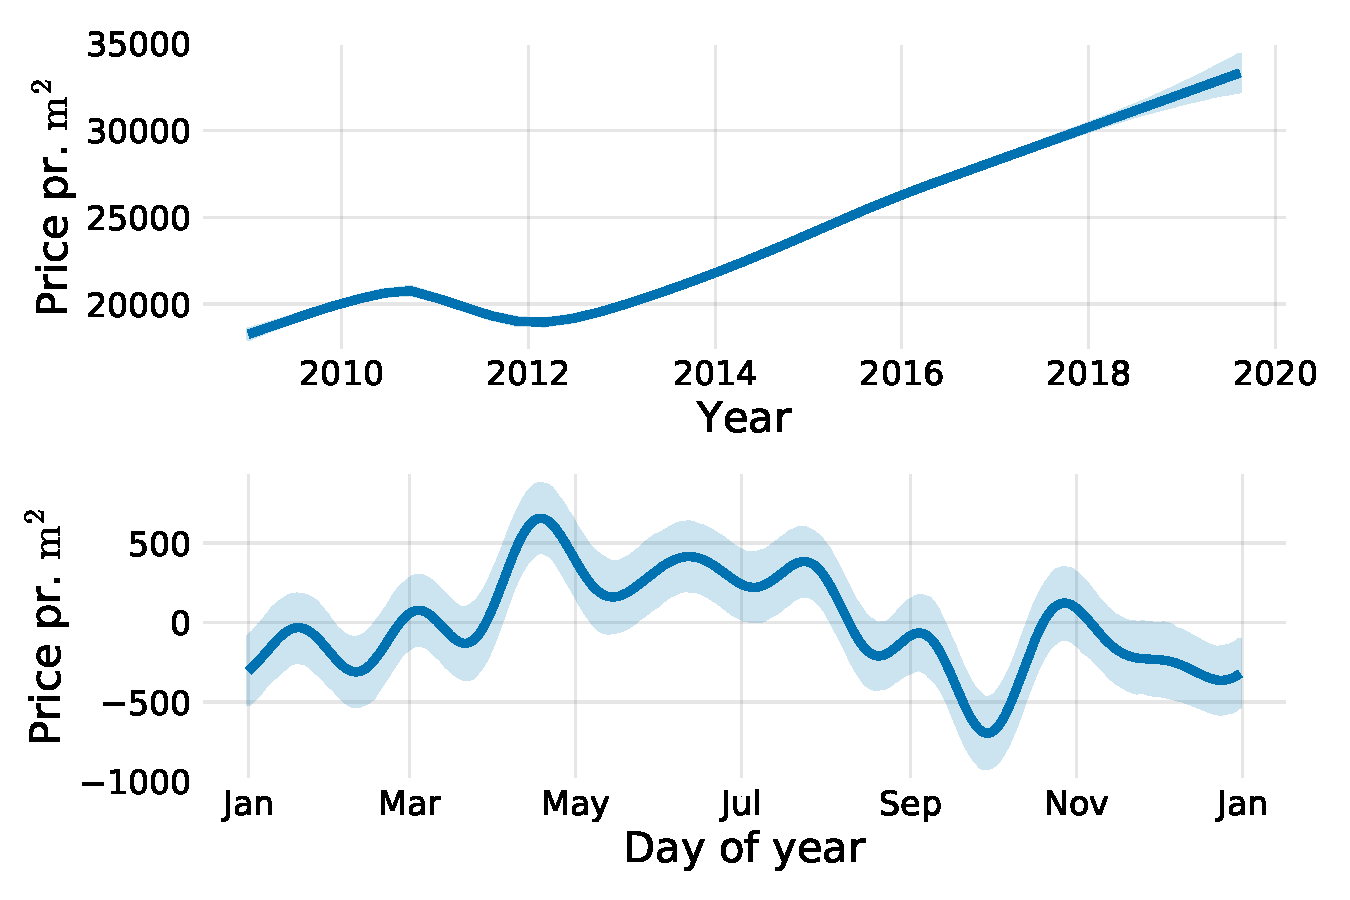
\includegraphics[draft=false, width=0.9\textwidth, trim=15 15 15 15, clip]{figures/housing/Ejerlejlighed_v18_cut_all_Ncols_all_prophet_trends.pdf}
  \caption[Prophet Trends]
          {The trends of the Facebook Prophet model trained on square meter prices for owner-occupied apartments sold before January 1st, 2018. In the top plot is the overall trend as a function of year and in the bottom plot is the yearly variation as a function of day of year. It can be seen that the square meter price is higher during the Summer months compared to the Winter months, however, compared to the overall trend this effect is minor ($<10\%$). 
          }
  \label{fig:h:prophet_trends}
\end{figure}

Using the Prophet model, we define the price index (PI) to be the Prophet-predicted PPSM, $y_\mathrm{Prophet}$, for each residence normalized by the mean to give values around \num{1}:
\begin{equation}
  % \mathrm{PI}(t) = \frac{y_\mathrm{Prophet}(t)}{\mathrm{mean}(y_\mathrm{Prophet}(t))}.
  \mathrm{PI}(t) = \frac{y_\mathrm{Prophet}(t)}{\langle y_\mathrm{Prophet}(t) \rangle},
\end{equation}
where $\langle \boldsymbol{\cdot} \rangle$ refers to the average. The price index thus works as a measure of the national price for houses or apartments at a given time and is added as a variable to the dataset. 

% \begin{figure}
%   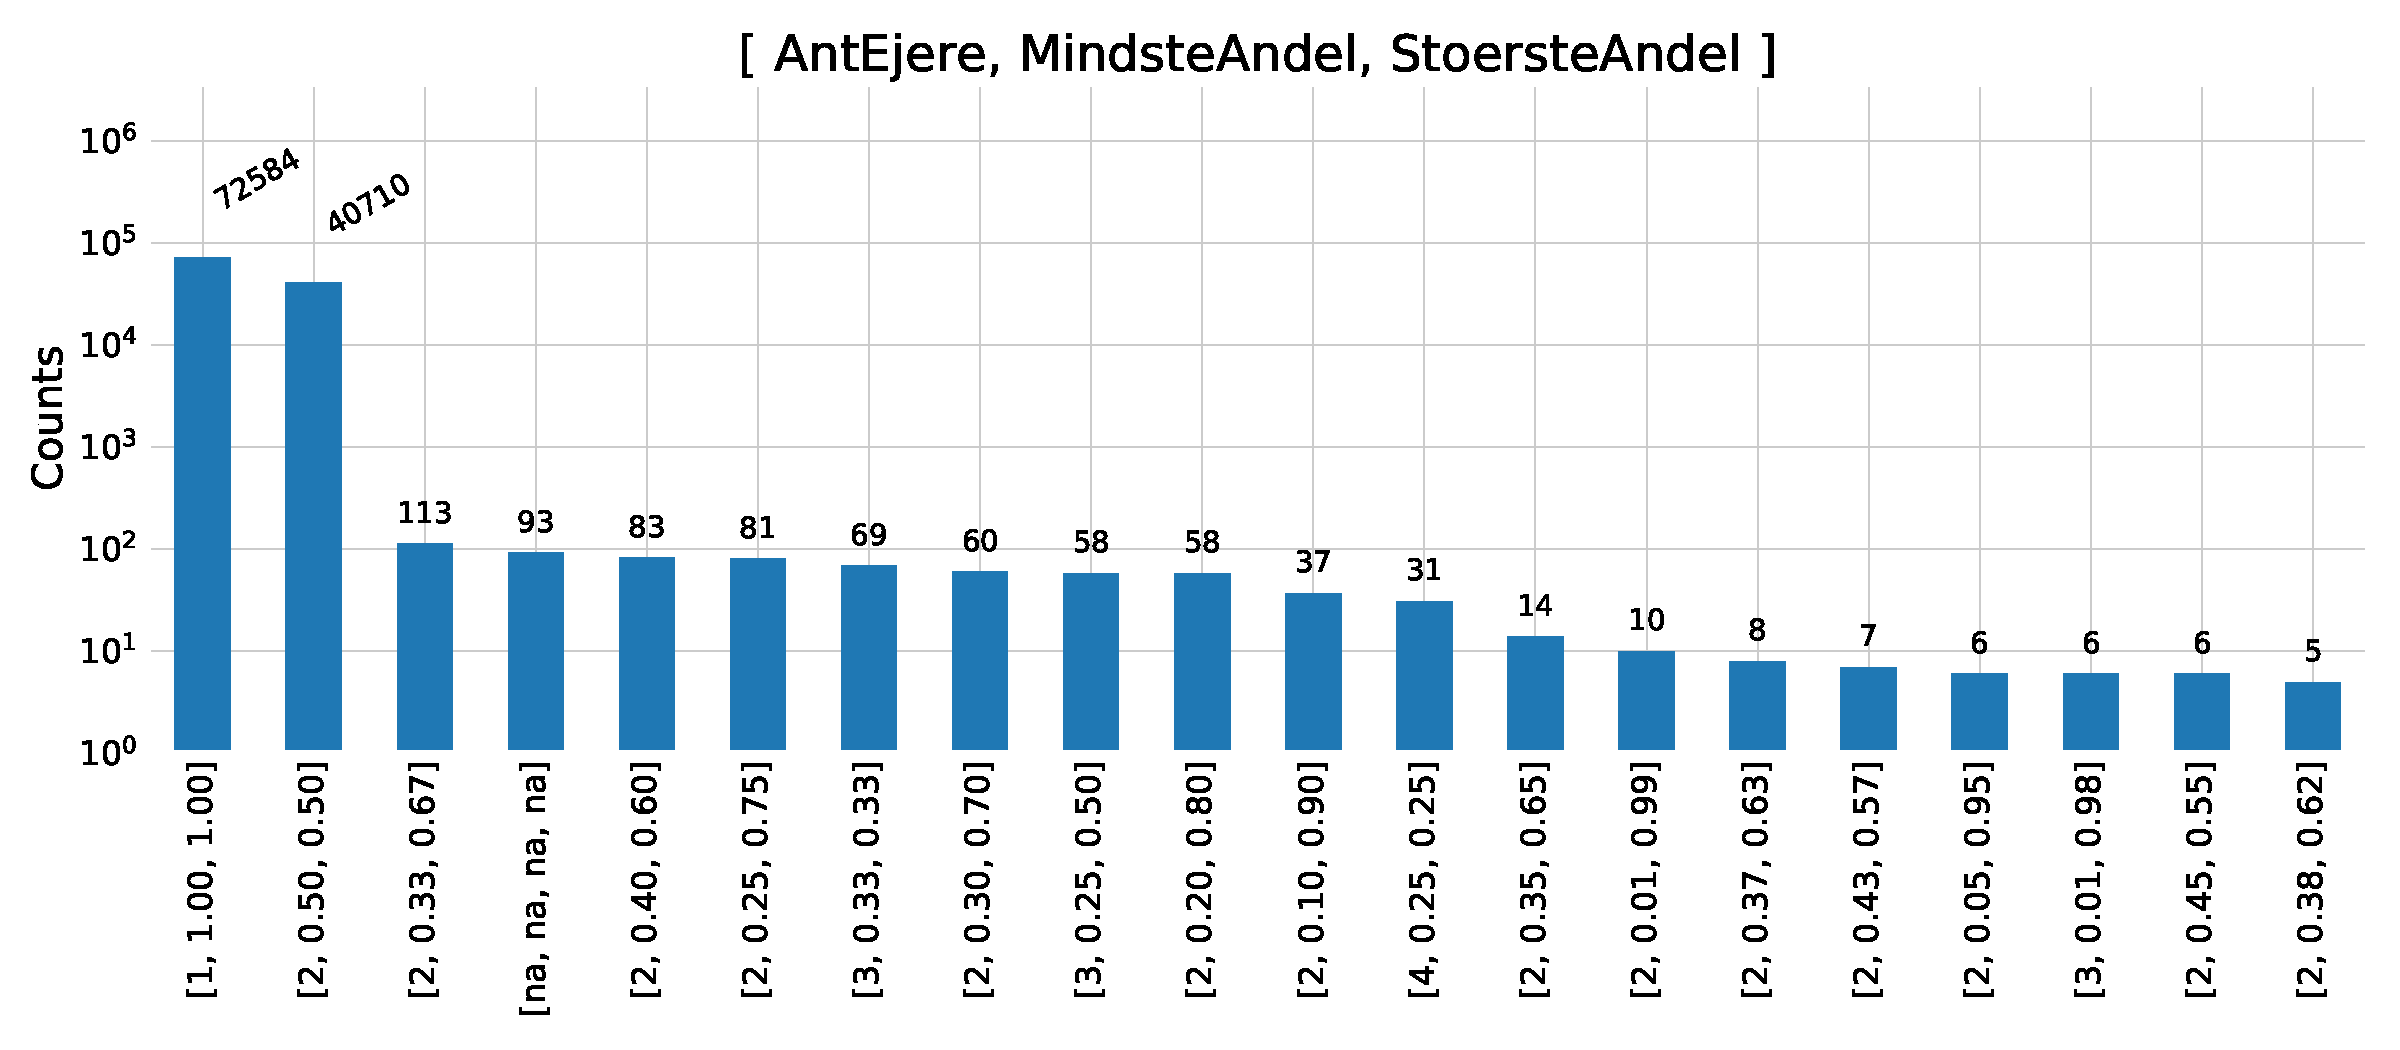
\includegraphics[width=0.9\textwidth]{figures/housing/tinglysning_fig.pdf}
%   \caption[Registration of property]
%           {Overview of registration of property as a function of amount of owners (\code{AntEjere}), lowest share (\code{MindsteAndel}) and biggest share (\code{StoersteAndel}) written as \code{[AntEjere, MindsteAndel, StoersteAndel]}.
%           }
%   \label{fig:h:tinglysning}
% \end{figure}

\section{Evaluation Function}
\label{sec:h:evaluation_function}

The choice of evaluation function $f_\mathrm{eval}$ is an important decision. The evaluation function will be based on the relative prediction $z$: 
\begin{equation}
  z = \frac{\hat{y}-y}{y},
\end{equation}
where $y$ is true price and $\hat{y}$ the predicted one. The relative prediction is defined such that it is positive when $\hat{y}>y$, due to the outlier cuts made earlier the denominator is made sure to always be positive (and never \num{0}), and $\vec{z}$ is expected to approximately follow a normal distribution\sidenote{Where $\vec{z}$ is the vector of all relative predictions $\vec{z} \in \mathbb{R}^N$.}. Initially the mean of $\vec{z}$ was considered as the choice of evaluation function $f_\mathrm{eval}\stackrel{?}{=} \mathrm{mean}(\vec{z})$ though this only ensures a minimum of bias, not necessarily a low spread. This lead the discussion on to look at the standard deviation of $z$ as $f_\mathrm{eval}\stackrel{?}{=} \mathrm{std}(\vec{z})$. The mean and the standard deviation, however, are not a very robust estimators since they are heavily influenced by outliers. The mean (and thus also the standard deviation) has a \emph{asymptotic breakdown point} at \SI{0}{\percent}, where the breakdown point is defined as the smallest fraction\sidenote{Where the \q{asymptotic} in \q{asymptotic breakdown point} refers to when the number of samples goes to infinity.} of bad observations that can cause an estimator to become arbitrarily small or large: a single outlier with an arbitrarily large value may cause the mean to diverge to that large value \autocite{huber2011robust}. In comparison, the median has an asymptotic breakdown point of \SI{50}{\percent} and is thus a more robust estimator of centrality. A robust measure of the variability or dispersion of a sample $\vec{x}$ -- compared to e.g. the standard deviation $\sigma$ -- is the median absolute deviation (MAD) written as:
\begin{equation}
  \mathrm{MAD}(\vec{x}) = c \cdot \mathrm{median} \left( \abs{\vec{x} - \mathrm{median}(\vec{x})} \right), \quad c = \frac{1}{\Phi^{-1}(\frac{3}{4})},
  \label{eq:h:MAD}
\end{equation}
where $c$ is a normalization constant to make MAD a consistent estimator of the standard deviation $\sigma$ assuming normally distributed data and $\Phi^{-1}$ is the percent point function\sidenote{Inverse of the cumulative distribution function.} \autocite{leysDetectingOutliersNot2013}.
The MAD is thus the median of the absolute differences between the data and the median of the data. We are, however, not just interested in having the distribution of $\vec{z}$ as narrow as possible, we also want it centered around \num{0}. We thus continue with the following evaluation function:
\begin{equation}
  \begin{split}
    \mathrm{MAD}_0(\vec{x})  &\equiv c \cdot  \mathrm{median} \left( \abs{\vec{x} - 0} \right) = c \cdot \mathrm{median} \left( \abs{\vec{x}} \right) \\
    f_\mathrm{eval}(\vec{z}) &\equiv \mathrm{MAD}_0(\vec{z}) = c \cdot  \mathrm{median} \left( \abs{\vec{z}} \right).
  \end{split}
\end{equation}
To get an intuition about the size of a \q{good} value of $\mathrm{MAD}_0$, one could calculate it comparing the asking price with the actual sales price. Doing so, one finds: $f_\mathrm{eval}(\vec{z}_\mathrm{OFH}) = \SI{11.35}{\percent}$ for houses and $f_\mathrm{eval}(\vec{z}_\mathrm{OOA}) = \SI{5.72}{\percent}$ for apartments. In some cases $f_\mathrm{eval}$ will still be referred to as MAD and it will be mentioned explicably if the form in equation \eqref{eq:h:MAD} is meant. 

\marginnote[-3cm]{The MAD is assuming symmetric distributions and thus non-symmetric robust measures of the variability of a sample have been developed. See \citet{rousseeuwAlternativesMedianAbsolute1993} for more details.}


\section{Initial Hyperparameter Optimization}
\label{sec:h:initial_hyperparameter_optimization}

With the initial cleaning and feature adding done, the shapes of the ML-ready datasets are: (\num{291317}, \num{144}) for houses (OFHs) and (\num{114166}, \num{144}) for apartments (OOA), both sharing the same variables. All of the variables which are used from this point on are shown in Table~\ref{tab:h:all_variables}. 
The data are split intro training and test sets such that training is defined as every sale from before \num{2018}, every sale from \num{2018} is the test set, and since more data came after the project started \num{2019} is a small extra test set. 

\begin{margintable}[-7cm]
  \begin{tabular}{lrr}
              & Houses       & Apartments   \\ \midrule
   Train      & \num{240070} & \num{93115}  \\   
   Test       & \num{34628}  & \num{14183}  \\   
   \num{2019} & \num{16619}  & \num{6868} 
  \end{tabular}
  \vspace{1.5mm}
  \caption[Number of Observations in the Housing Dataset]{\label{tab:h:train_test_split}Number of observations for houses and apartments in the training, test, and \num{2019} set.}
  \vspace{3mm}
\end{margintable}

\begin{margintable}[-2cm]
  \begin{tabular}{lrr}
% \begin{table}
  % \begin{tabular}{lll}
   Tight      & Houses        & Apartments  \\ \midrule
   Train      & \num{143179}  & \num{57795} \\   
   Test       & \num{20338}   & \num{8376}  \\   
   \num{2019} & \num{9683}    & \num{4030} 
  \end{tabular}
  \vspace{1.5mm}
  \caption[Number of Observations in the Housing Dataset for the Tight Selection]{\label{tab:h:train_test_split_tight}Number of observations for houses and apartments in the training, test, and \num{2019} set for the tight selection.}
  \vspace{3mm}
\end{margintable}

The number of observations for the different sets are shown in Table~\ref{tab:h:train_test_split}. Since the dataset has been shown to be quite noisy with a lot of invalid counts a \emph{tight} selection of the data is also applied. The tight selection is defined as residences which are within the \SI{1}{\percent} to \SI{99}{\percent} quantiles of all\sidenote[][-0.5cm]{Except the variables that contains the words: \q{aar} (year), \q{dato} (date), and  \q{prophet}.} numeric variables with more than 3 unique values. The number of observations for the different tight sets are shown in Table~\ref{tab:h:train_test_split_tight}. 

A small study into the effect of some various hyperparameters was performed before any further fitting. This study investigated the effect of the old sales by assigning them a lower weight depending on time. It was investigated whether or not the model would perform better if samples got the time-dependent weight $w(t)$ given by:
\begin{equation}
  \begin{split}
    w'(t) &= e^{ k \cdot t}, \quad k = \frac{\log 2}{T_{\frac{1}{2}}} \, ,\\
    w(t) &= \frac{w'(t)}{\langle w'(t) \rangle} \, ,
  \end{split}
  \label{eg:h:sample_weight}
\end{equation}
% TODO: add parts about what weights are.
\begin{marginfigure}[-4cm]
  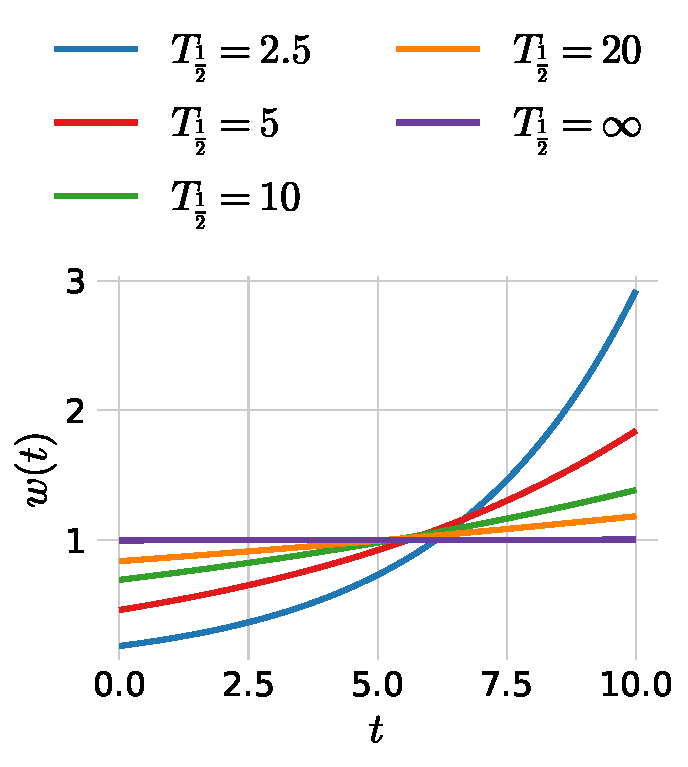
\includegraphics[width=0.99\textwidth]{figures/housing/Villa_v18_cut_all_Ncols_all_half_life_weights.pdf}
  \caption[Sample Weight as a Function of Time for Different Half-Lives.]
    {The sample weight $w(t)$ as a function of time $t$ where the time is in years after January \nth{1}, 2009, Here seen plotted for different values of the half-life $T_{\frac{1}{2}}$.}
  \label{fig:h:half-life}
\end{marginfigure}
\noindent where $T_{\frac{1}{2}}$ is the half-life. This is illustrated in Figure~\ref{fig:h:half-life} for the different values of $T_{\frac{1}{2}}$ used in the study.  In addition to the weight, it was also investigated whether or not a $\log_{10}$-transformation of the price would increase performance. The reasoning behind this would be that some machine learning methods assume that the dependent variable, $y$, is normally distributed. Finally the choice of loss function was also added to the study for the five different loss functions defined in \autoref{sec:ml:loss_function}. A grid search\sidenote[][-2cm]{Grid search was acceptable since the parameter space is small and two of the three dimensions are non-numerical.} was performed for:
\begin{equation}
  \begin{split}
    T_{\frac{1}{2}} &\in \{2.5,\, 5,\, 10,\, 20,\, \infty \}~\mathrm{ years} \\
    \log_{10} &\in \{\mathrm{True},\, \mathrm{False} \} \\
    \ell &\in \{ \ell_\mathrm{Cauchy},\, \ell_\mathrm{Fair},\, \ell_\mathrm{LogCosh},\, \ell_\mathrm{SE},\, \ell_\mathrm{Welsch}\}.
  \end{split}
\end{equation}

\begin{margintable}[-1cm]
  \begin{tabular}{@{}ccrc@{}}
    %\toprule
    Half-life & $\log_{10}$ & $N_\mathrm{trees}$ & $f_\mathrm{eval}$ \\
    \midrule
    \num{2.5} & True & \num{293} & \num{0.1598} \\
    \num{2.5} & False & \num{814} & \num{0.1466} \\
    \num{5} & True & \num{304} & \num{0.1610} \\
    \num{5} & False & \num{923} & \num{0.1468} \\
    \num{10} & True & \num{266} & \num{0.1610} \\
    $\mathbf{10}$ & \textbf{False} & $\mathbf{770}$ & $\mathbf{0.1450}$ \\
    \num{20} & True & \num{288} & \num{0.1613} \\
    \num{20} & False & \num{967} & \num{0.1467} \\
    $\infty$ & True & \num{340} & \num{0.1601} \\
    $\infty$ & False & \num{807} & \num{0.1480} \\
    %\bottomrule
  \end{tabular}
  \vspace{1.5mm}
  \caption[Results from the Initial Hyperparameter Optimization for Apartments]{\label{tab:h:HPO_initial_Cauchy-ejerlejlighed}Results of the initial hyperparameter optimization for apartments for the best loss function $\ell_\mathrm{Cauchy}$. The best hyperparameter is shown in bold.}
\end{margintable}


\begin{margintable}[0.5cm]
  \begin{tabular}{@{}ccrc@{}}
    %\toprule
    Half-life & $\log_{10}$ & $N_\mathrm{trees}$ & $f_\mathrm{eval}$ \\
    \midrule
    \num{2.5} & True & \num{434} & \num{0.1991} \\
    \num{2.5} & False & \num{1007} & \num{0.1872} \\
    \num{5} & True & \num{350} & \num{0.1999} \\
    \num{5} & False & \num{1130} & \num{0.1858} \\
    \num{10} & True & \num{436} & \num{0.1992} \\
    \num{10} & False & \num{1183} & \num{0.1850} \\
    \num{20} & True & \num{397} & \num{0.2003} \\
    $\mathbf{20}$ & \textbf{False} & $\mathbf{1514}$ & $\mathbf{0.1833}$ \\
    $\infty$ & True & \num{449} & \num{0.1992} \\
    $\infty$ & False & \num{1351} & \num{0.1844} \\
    %\bottomrule
  \end{tabular}
  \vspace{1.5mm}
  \caption[Results from the Initial Hyperparameter Optimization for Houses]{\label{tab:h:HPO_initial_Cauchy-villa}Results of the initial hyperparameter optimization for houses for the best loss function $\ell_\mathrm{Cauchy}$. The best hyperparameter is shown in bold.}
\end{margintable}


The grid search is run on the training set with \num{5}-fold cross validation, early stopping is applied with a patience of \num{100}, and XGBoost \autocite{chenXGBoostScalableTree2016} (XGB) is used as the ML model. For apartments the loss function with the lowest $f_\mathrm{eval}$ was the Cauchy loss with $T_{\frac{1}{2}}=10$ years and no $\log_{10}$-transformation. This BDT terminated by early stopping after \num{770} trees, see Table~\ref{tab:h:HPO_initial_Cauchy-ejerlejlighed}. 
For houses the loss function with the lowest $f_\mathrm{eval}$ was (also) the Cauchy loss with $T_{\frac{1}{2}}=20$ years and (also) no $\log_{10}$-transformation. This BDT terminated by early stopping after \num{1514} trees, see Table~\ref{tab:h:HPO_initial_Cauchy-villa}. 
It is interesting to note that both HPO for houses and apartments choose the same loss function and not to do any transformation. 

The reason why the $\log_{10}$-transformation was included even to begin with, was that initially it showed better results than no transformation, however, this turned out to be a numerical consequence which was alleviated by dividing all prices with a million, such that $y$ had units of \si{\Mkr} instead of \si{\kr}. All of the results for the apartments are shown in Table~\ref{tab:h:HPO_initial_Rmse-ejerlejlighed-appendix}--\ref{tab:h:HPO_initial_Fair-ejerlejlighed-appendix} along with all of results for the houses in Table~\ref{tab:h:HPO_initial_Rmse-villa-appendix}--\ref{tab:h:HPO_initial_Fair-villa-appendix}. 

\begin{figure}[h!]
  \centerfloat
  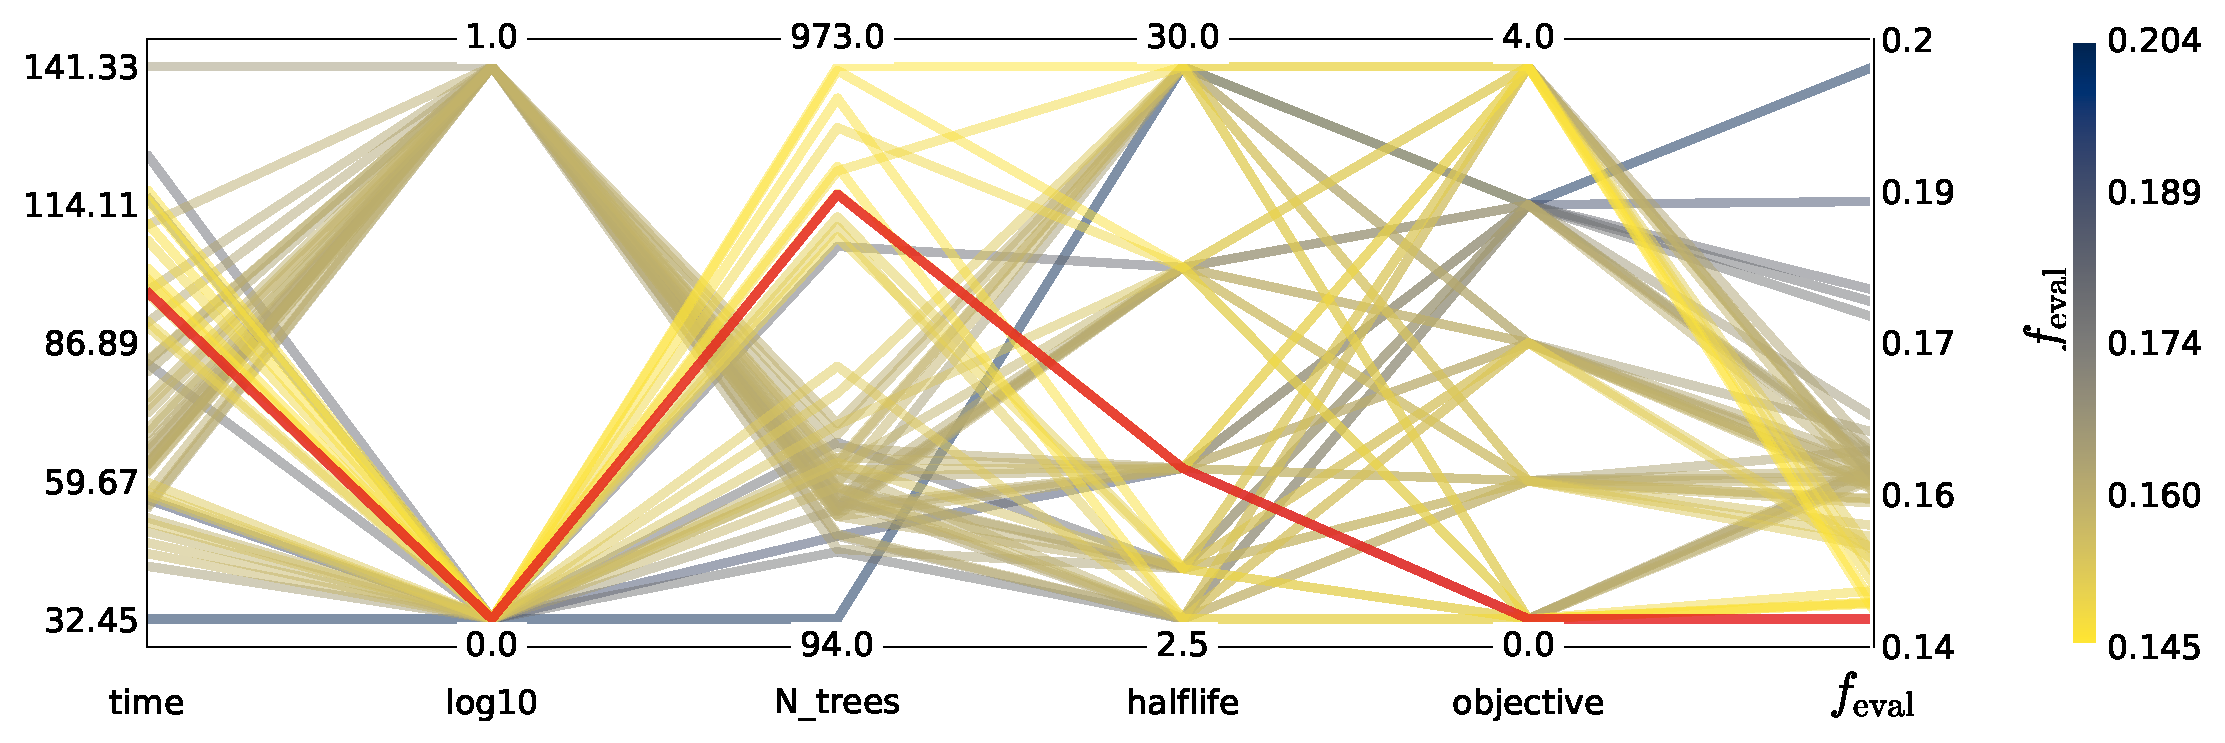
\includegraphics[width=0.99\textwidth, trim=0 0 0 0, clip]{figures/housing/Ejerlejlighed_v19_cut_all_Ncols_all_CV_viz_initial_HPO.pdf}
  \caption[Parallel Coordinate Plot of the Initial Hyperparameter Optimization for Apartments]
          {Hyperparameter optimization results for apartments. The results are shown as parallel coordinates with each hyperparameter along the $x$-axis and the value of that parameter on the $y$-axis. Each line is an iteration of the RS HPO colored according to the performance of that hyperparameter as measured by the MAD from \textcolor{viridis-dark}{highest} in dark blue to \textcolor{viridis-light}{lowest (best)} in yellow. The \textcolor{red}{single best hyperparameter} is shown in red. For the hyperparameter \code{log10} \code{0} means False and \code{1} means True, for \code{Halftime} $\infty$ is mapped to \code{30}, and for \code{objective} the functions Cauchy (0), Fair (1), LogCosh (2) SquaredError (3), and Welsch (4) are mapped to the integers in the parentheses.
          } 
  \label{fig:h:initial_CV_res_parallel_coords_ejer}
\end{figure}

The HPO results are shown in the parallel coordinate plot in Figure~\ref{fig:h:initial_CV_res_parallel_coords_ejer}. Here the hyperparameters (along the time taken and the number of trees) of the HPO are plotted along the abscissa (x-axis) and the value of the hyperparameter on the ordinate (y-axis). Every iteration of the HPO is thus a line on the plot. The lines are colored according to their evaluation score; the best hyperparameter is shown in red. For the hyperparameter \code{log10} \code{0} means False and \code{1} means True, for \code{Halftime} $\infty$ is mapped to \code{30}, and for \code{objektive} the functions Cauchy (0), Fair (1), LogCosh (2) SquaredError (3), and Welsch (4) are mapped to the integers in the parentheses. The HPO results for houses is shown in Figure~\ref{fig:h:initial_CV_res_parallel_coords_villa}.


What can be concluded from Figure~\ref{fig:h:initial_CV_res_parallel_coords_ejer} is that there is a clear preference to not $\log$-transform the data, that the BDTs with many trees\sidenote{Remember that the number of trees were selected by early stopping.} generally performed better than the ones with fewer trees, that it is difficult to see a clear pattern for the half-life, and that there seems to be a tendency for the Cauchy loss to be the best, however, it is still ambiguous. What is not seen in the figure, however, are how the uncertainties of the different iterations also matter, where the uncertainties are the standard deviations (not of the mean) of the \num{5} folds in the cross validation.
\begin{marginfigure}
  \centerfloat
  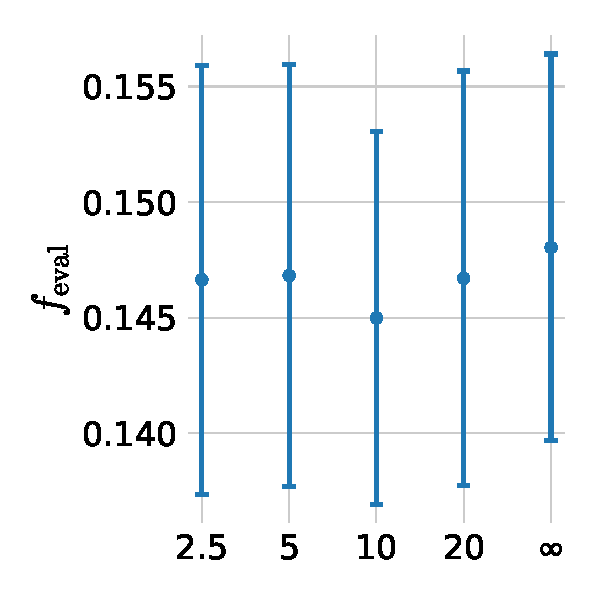
\includegraphics[width=0.95\textwidth, trim=0 0 0 0, clip]{figures/housing/Ejerlejlighed_v19_cut_all_Ncols_all_MAD_gridsearch_half.pdf}
  \caption[Initial HPO Results for the Weight Half-life $T_{\frac{1}{2}}$]
          {Evaluation score as a function of the weight half-life $T_{\frac{1}{2}}$ with the standard deviation over the \num{5} folds as errorbars for apartments.}
  \label{fig:h:hpo_gridsearch_objective}
\end{marginfigure}

\begin{marginfigure}
  \centerfloat
  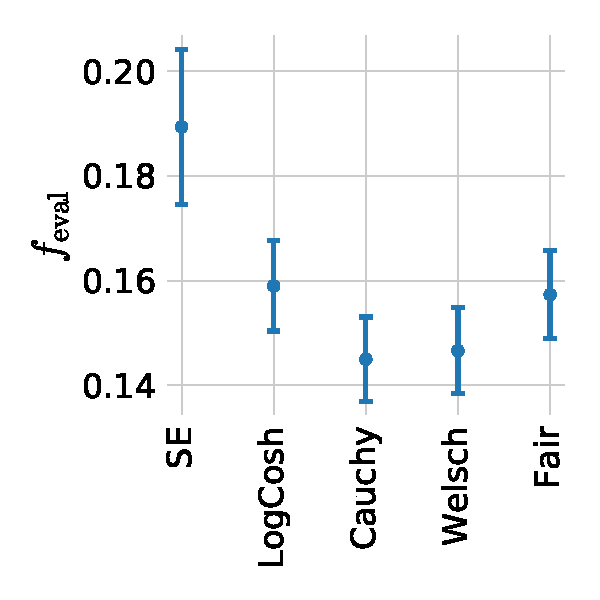
\includegraphics[width=0.95\textwidth, trim=0 0 0 0, clip]{figures/housing/Ejerlejlighed_v19_cut_all_Ncols_all_MAD_gridsearch_obj.pdf}
  \caption[Initial HPO Results for the Loss Function]
          {Evaluation score as a function of the loss function with the standard deviation over the \num{5} folds as errorbars for apartments.}
  \label{fig:h:hpo_gridsearch_halflife}
\end{marginfigure}

For the half-life and the choice of objective function these are shown in Figure~\ref{fig:h:hpo_gridsearch_objective} and \ref{fig:h:hpo_gridsearch_halflife}. In the first of the two figures it is easily seen that even though $T_{\frac{1}{2}}=\SI{10}{\yr}$ is the minimum, the uncertainties are so large that nothing can be concluded definitely with regards to the half-life parameter related to the weights $w(t)$. In contrary, in the second figure there is a clear performance difference between the different loss functions where the Cauchy loss archives the best (lowest) value of $f_\mathrm{eval}$ and especially the Squared Error is disregarded. 

The rest of the machine learning models thus continue with the following hyperparameters:

\begin{table}[h]
  \centerfloat
  \begin{tabular}{@{}llcl@{}}
               & $\log_{10}$  & Half-life & Loss function \\ \midrule
  Apartments   & False & \SI{10}{\yr} & Cauchy \\
  Houses       & False & \SI{20}{\yr} & Cauchy
  \end{tabular}
  \label{tab:h:initial_hpo}
\end{table}



\FloatBarrier
\section{Hyperparameter Optimization}
\label{sec:h:hyperparamater_optimization}
With the initial HPO set, the actual training of the models was started. An XGBoost model was fitted to the each of the two training sets, one for apartments and one for houses, where the hyperparameters were optimized using both random search and Bayesian optimization each run for \num{100} iterations with \num{5}-fold cross validation and early stopping\sidenote{This takes a good \num{4} hours for the RS, \num{7} hours for the BO, and \num{90} minutes to optimize the learning rate with early stopping for apartments when run on the local computing cluster, HEP. For the houses this takes a good \num{24} hours for the RS, \num{34} hours for the BO, and almost \num{5} hours optimize the learning rate with early stopping.}. The hyperparameters to be optimized were the following:
\begin{itemize}
  \item[] The \code{subsample} variable controls the row-subsampling and is a number between \num{0} and \num{1}. 
  \item[] The hyperparameter \code{colsample_bytree} controls the column downsampling for each tree, so how many columns (or variables) each tree are allowed to fit to. Is a number between \num{0} and \num{1}.
  \item[] The \code{max_depth} controls the maximum depth of every tree. Is a positive integer (negative values means no maximum depth).  
  \item[] The \code{min_child_weight} variable controls when the decision tree algorithm should stop splitting a node into further nodes (and will thus turn it into a leaf). Is a positive integer.
  \item[] \code{reg_lambda} controls the L2 regularization term. Is a positive number. 
  \item[] \code{reg_alpha} controls the L1 regularization term. Is a positive number.
\end{itemize}

The ranges of the hyperparameters were chosen by a manual, iterative process of fitting a subset of the data (\SI{1}{\percent}--\SI{10}{\percent}) and making sure that the best hyperparameter is not sufficiently close to the range; if it is, then the range is extended. The final HPO ranges chosen are shown in Table~\ref{tab:h:hpo_ranges}. Here $\mathcal{U}(a, b)$ refers to a uniform distribution from $a$ to $b$, and $\mathcal{U}_\mathrm{int}(a, b)$ is the same only an integer distribution. 
\begin{margintable}
  \centerfloat
  \begin{tabular}{@{}ll@{}}
  Hyperparameter          &  Range                      \\ \midrule
  \code{subsample}        & $\mathcal{U}(0.5, 0.9)$           \\
  \code{colsample_bytree} & $\mathcal{U}(0.1, 0.99)$           \\
  \code{max_depth}        & $\mathcal{U}_\mathrm{int}(1, 20)$ \\
  \code{min_child_weight} & $\mathcal{U}_\mathrm{int}(1, 30)$ \\
  \code{reg_lambda}       & $\mathcal{U}(0.1, 4)$  \\
  \code{reg_alpha}        & $\mathcal{U}(0.1, 4)$
  \end{tabular}
  % \vspace{\abovecaptionskip}
  \vspace{3mm}
  \caption[PDFs Used in the Random Search]{\label{tab:h:hpo_ranges} Probability Density Functions used in the random search to draw new sets of values for the hyperparameters. Each hyperparameter is drawn from the distribution seen in the table.}
\end{margintable}

The fitting pipeline for this subproject is to first run both RS and BO as HPOs to compare their results. The best of the two models is chosen and finally learning rate optimized by early stopping where the learning rate $\eta$ is reduced from $\eta=0.1$ to $\eta=0.01$. In the end one ends up with a model that has been HPO optimized for preprocessing optimizations, loss functions, sample weights, normal BDT hyperparameters and finally the learning rate. I have manually implemented this pipeline in Python since no other packages provide the same flexibility as a custom implementation that works fully automatically. 

The results of the RS and BO are shown in Figure~\ref{fig:h:CV_res_RS_parallel_coords_ejer_non_appendix} and \ref{fig:h:CV_res_BO_parallel_coords_ejer}. The corresponding plots for houses are shown in Figure~\ref{fig:h:CV_res_RS_parallel_coords_villa} and \ref{fig:h:CV_res_BO_parallel_coords_villa}. 

\begin{figure}
  \centerfloat
  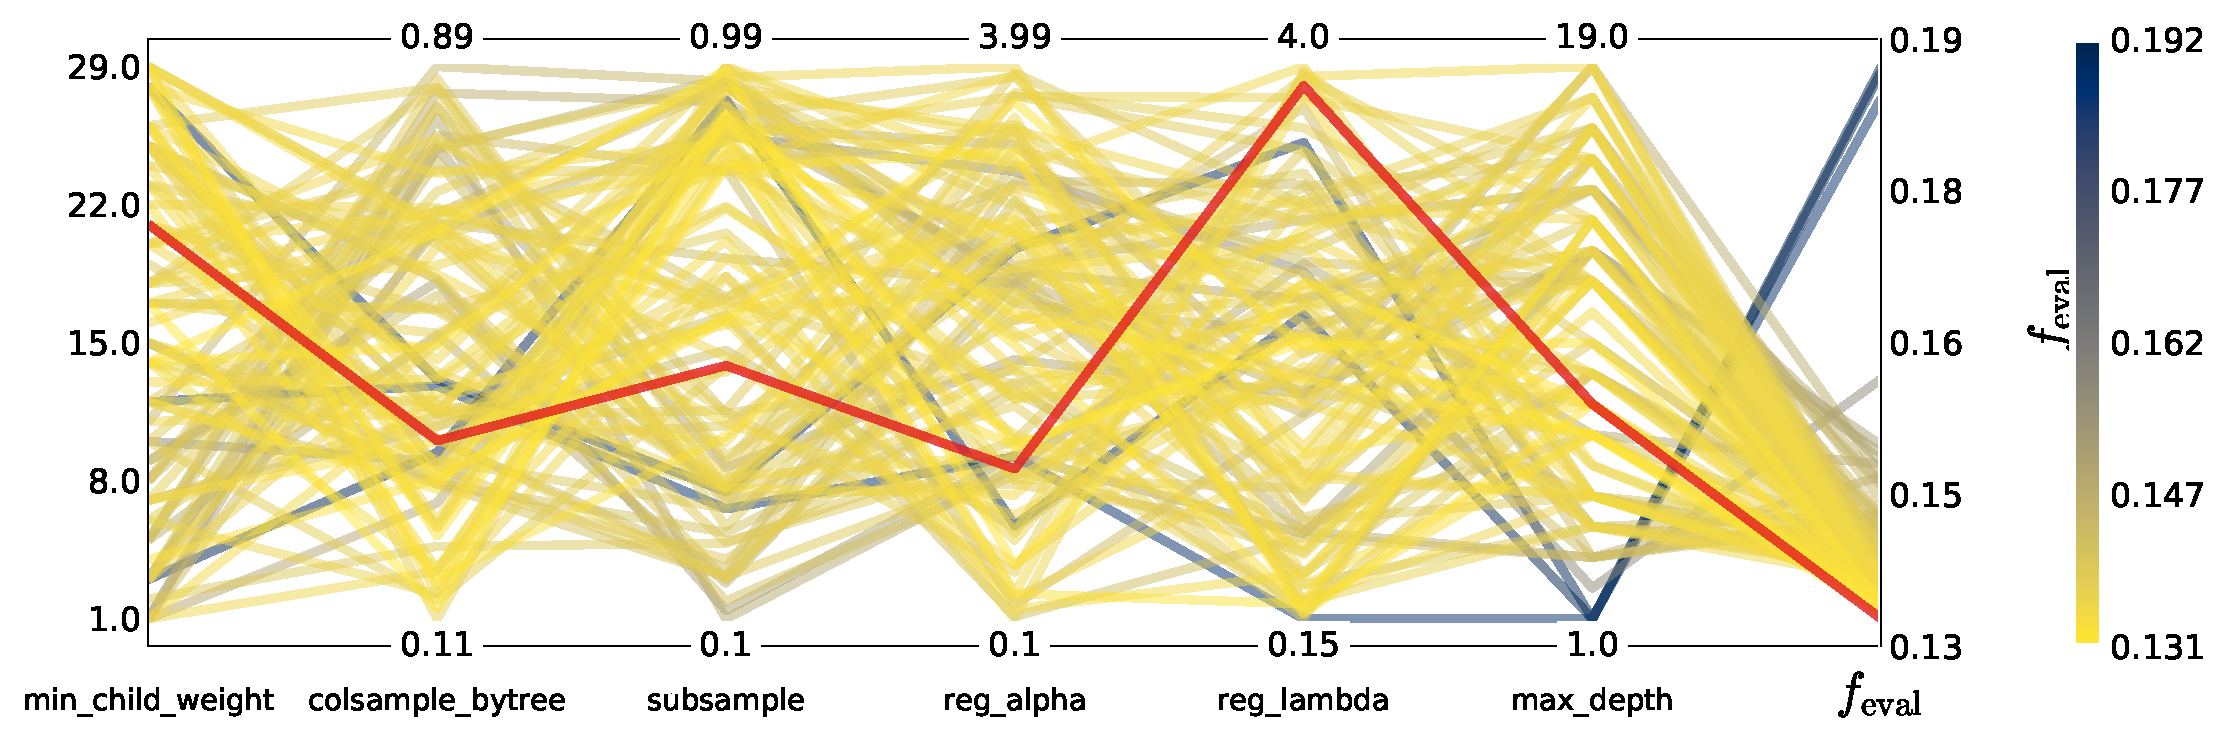
\includegraphics[width=0.99\textwidth, trim=0 0 0 0, clip]{figures/housing/Ejerlejlighed_v19_cut_all_Ncols_all_CV_viz_HPO_RS.pdf}
  \caption[Parallel Coordinate Plot of the Random Search Hyperparameter Optimization Results of XGBoost for Apartments]
          {Hyperparameter optimization results of XGBoost parameters of the housing model for apartments shown as parallel coordinates. Here shown for random search as hyperparameter optimization. } 
  \label{fig:h:CV_res_RS_parallel_coords_ejer_non_appendix}
\end{figure}

As with the initial HPO, it is important to compare the results in Figure~\ref{fig:h:CV_res_RS_parallel_coords_ejer_non_appendix} with their uncertainties. This is shown in Figure~\ref{fig:h:CV_res_RS_uncertainties_ejer}. Here the value of the evaluation function along with its \num{1}$\sigma$  and \num{2}$\sigma$ uncertainties are plotted as a function of the iteration along the abscissa. The minimum value of $f_\mathrm{eval}$ is shown in red. Even though this is the minimum value, notice how most of the other iterations are within \num{1}$\sigma$. The plot for BO in Figure~\ref{fig:h:CV_res_BO_uncertainties_ejer} shows the exploration phase in the first half of the iterations where it afterwards converge to a more flat minimum, however, this minimum was still worse than the one found with RS. 

\begin{figure}
  \centerfloat
  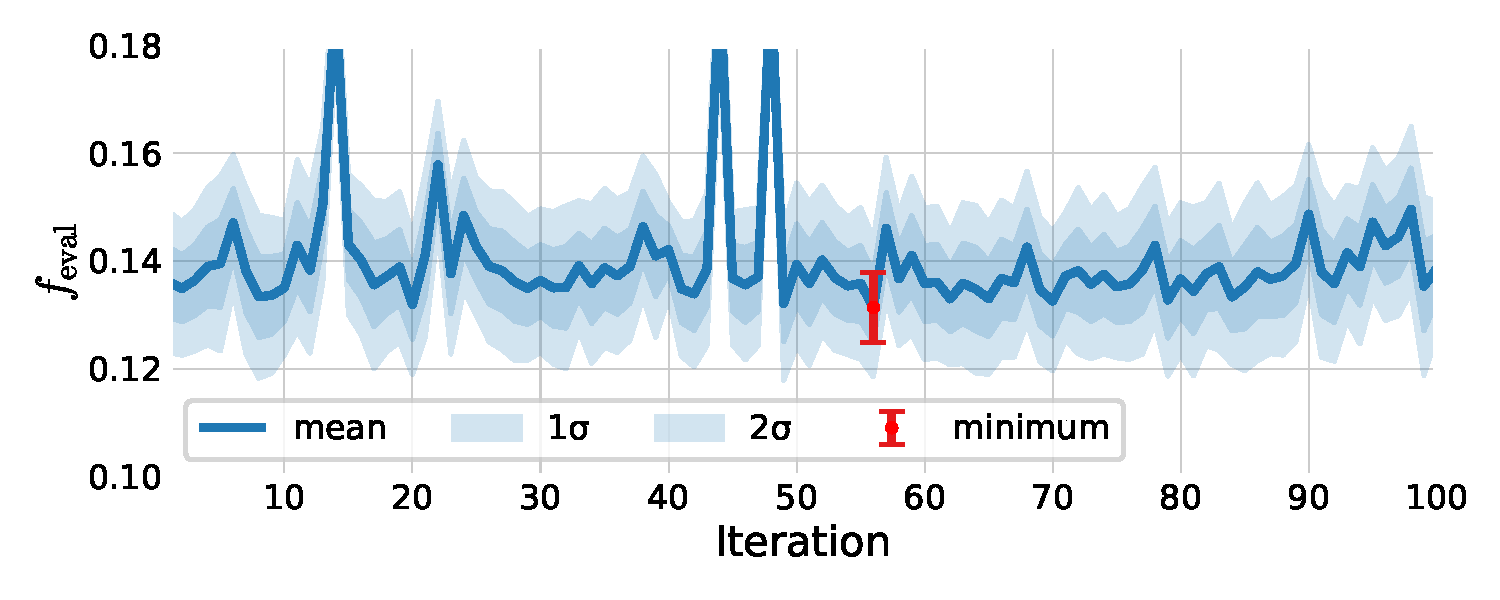
\includegraphics[width=0.95\textwidth, trim=10 20 10 10, clip]{figures/housing/Ejerlejlighed_v19_cut_all_Ncols_all_xgb_score_over_time_random.pdf}
  \caption[Hyperparameter Optimization: Random Search Results]
          {The results of running random search (RS) as hyperparameter optimization (HPO) on apartments using the XGB-model. The \textcolor{red}{minimum (mean) loss} along with its uncertainty is shown in red, the \textcolor{blue}{means} for the different iterations of RS in blue, and as light blue bands are the \textcolor{blue}{one (and two) standard deviation(s)}, all as a function of iteration number.} 
  \label{fig:h:CV_res_RS_uncertainties_ejer}
\end{figure}

The best of the RS and GS models are chosen for subsequent analysis by first reducing the learning rate to $\eta=0.01$ and then find the best number of estimators by early stopping. The evaluation function as a function of number of estimators, also known as the \emph{learning curve}, is seen in Figure~\ref{fig:h:CV_res_ES_learning_curve_ejer}. This curve is the realization of Figure~\ref{fig:ml:empirical_risk} in real data, where it first improves a lot and then finds a stable plateau. The minimum is shown in red with its uncertainty. To reduce the risk of overfitting and model complexity -- with the further advantage of resulting in a faster model at prediction time -- we keep the model with the lowest number of estimators that are still within $1\sigma$ of the minimum: see the orange point in the figure. This results in a model that contains less than a fifth of the number of trees and is thus also significantly simpler and faster at inference time. This is the final hyperparameter optimized model that will be used for the further analysis. 

\begin{figure}
  \centerfloat
  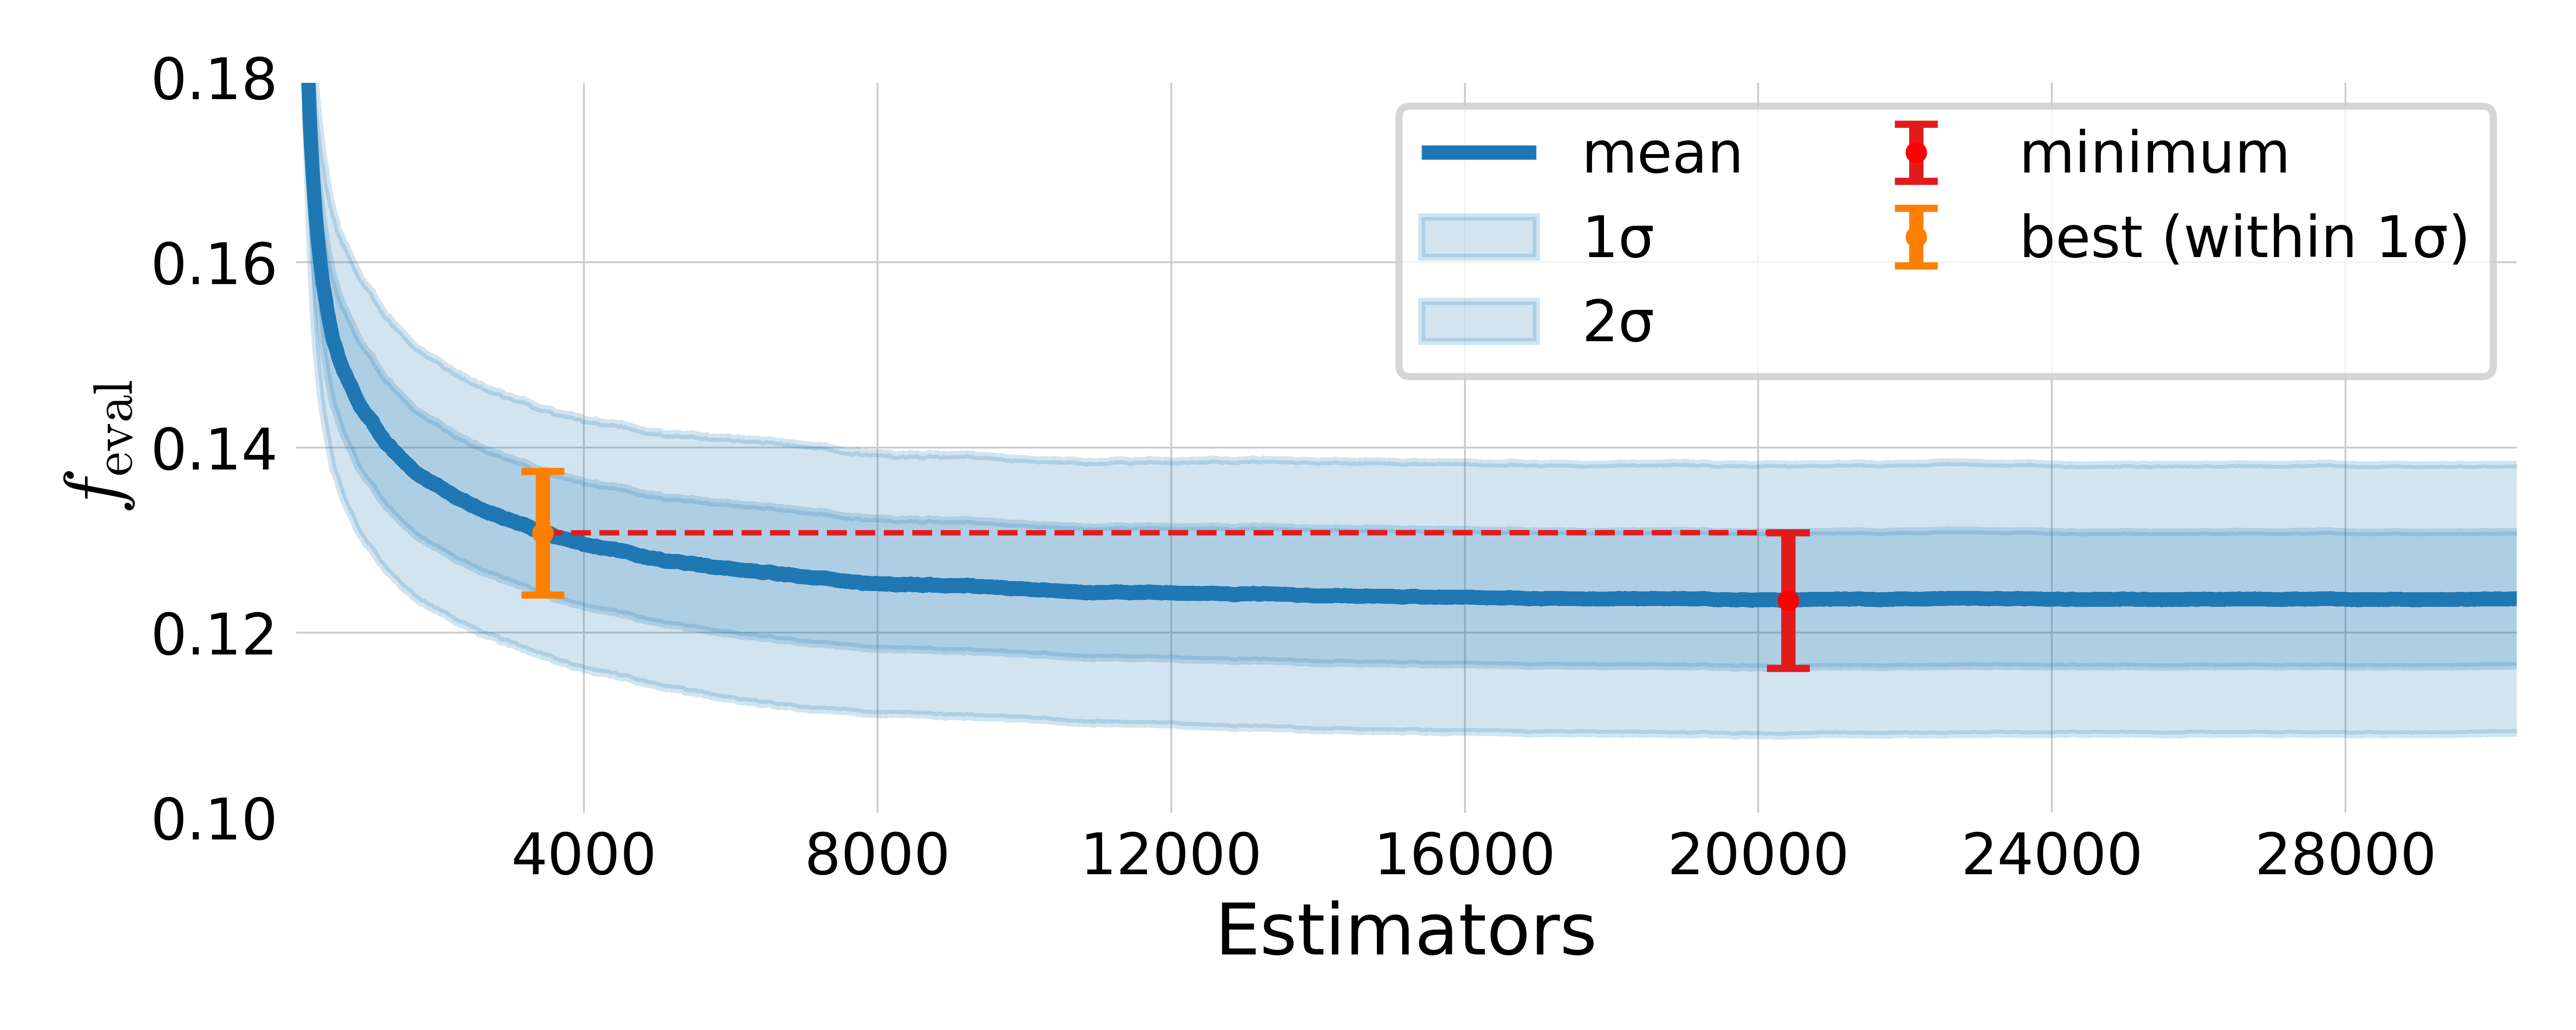
\includegraphics[draft=false, width=0.99\textwidth, trim=10 20 10 10, clip]{figures/housing/Ejerlejlighed_v19_cut_all_Ncols_all_xgb_early_stopping_fig.png}
  \caption[Early Stopping Results]
          {The results of early stopping on apartments using the XGB-model. The \textcolor{red}{minimum (mean) loss} along with its uncertainty is shown in red, the \textcolor{blue}{means} for the different iterations of RS in blue, and as light blue bands are the \textcolor{blue}{one (and two) standard deviation(s)}, all as a function of number of estimators (trees). In orange the \textcolor{orange}{\q{best} number of estimators} is shown, defined as the lowest number of estimators which are still within $1\sigma$ of the minimum value.} 
  \label{fig:h:CV_res_ES_learning_curve_ejer}
\end{figure}

\vspace{-0.5cm}


\FloatBarrier
\section{Results}
\label{sec:h:results}

The performances of the different models, the random search optimized, the bayesian optimization optimized and the best of the two $\eta$ optimized with early stopping, are shown in Figure~\ref{fig:h:CV_res_performance_ejer}. Here the distribution of the relative price prediction $\vec{z}$ of the model evaluated on the test set, apartments sold in \num{2018}, is shown for the three models. In addition to the distributions, also the performance metrics are shown: the value of the evaluation function\sidenote{Written as \code{MAD}.} along with the fraction of relative price predictions that are within the specified percentage. In this particular instance it is seen that \SI{41.3}{\percent} of the predictions by the final early stopping model are less than $\pm\SI{5}{\percent}$ wrong, \SI{69.8}{\percent} within $\pm\SI{10}{\percent}$, and \SI{91.9}{\percent} within $\pm\SI{20}{\percent}$. Note that the differences between the three models are minor and that the distributions almost cannot be distinguished from each other. 

\begin{figure}[h!]
  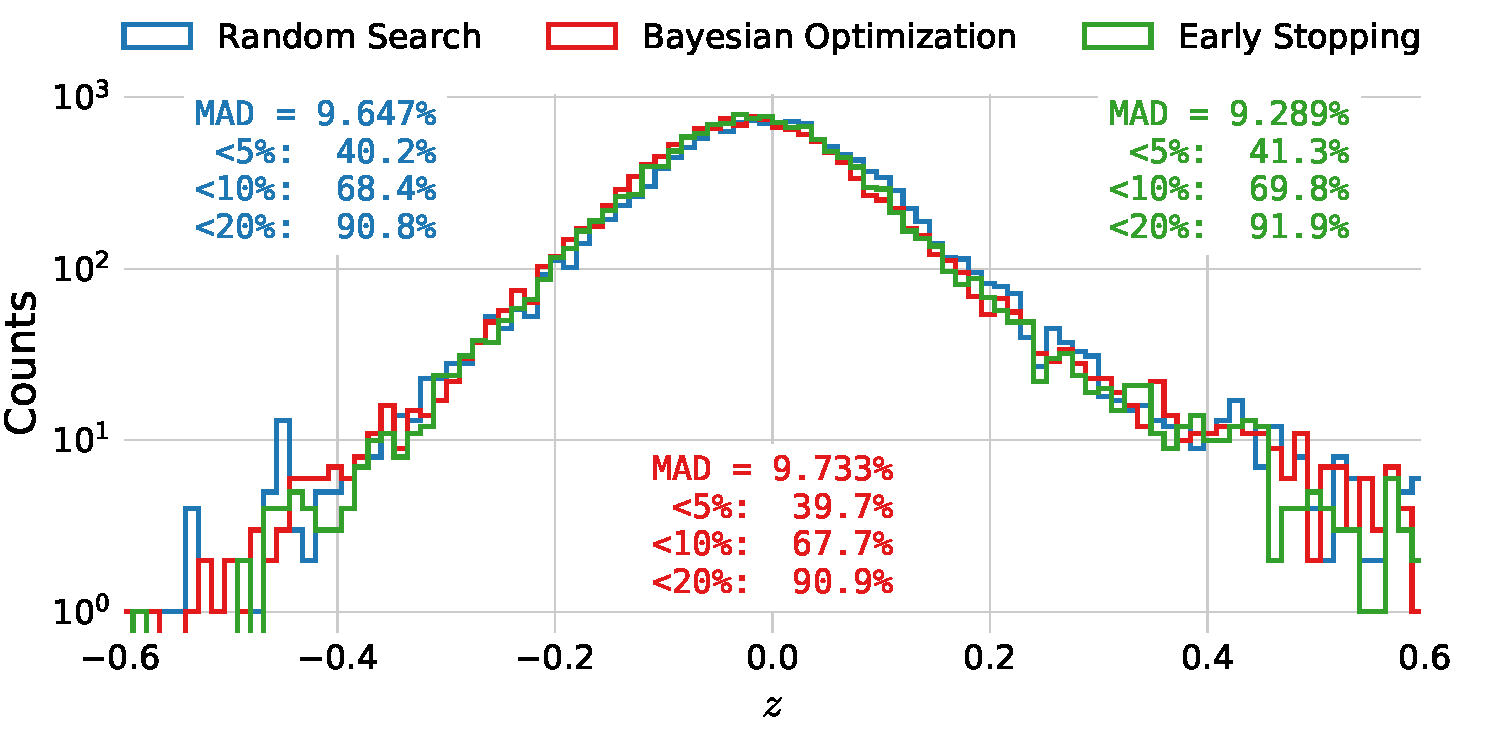
\includegraphics[width=0.95\textwidth, trim=0 10 10 5, clip]{figures/housing/Ejerlejlighed_v19_cut_all_Ncols_all_xgb_z_hist_metrics.pdf}
  \caption[Performance of XGB-model for Apartments]
          {Histogram of $z$-values of the XGB-model trained on apartments. The performance after hyperparameter optimization using \textcolor{blue}{random search} is shown in blue, for \textcolor{red}{Bayesian optimization} in red, and the learning rate optimized with \textcolor{green}{early stopping} in green.
          } 
  \label{fig:h:CV_res_performance_ejer}
\end{figure}

An interesting observation from the performance metrics of the test set is the low value of $f_\mathrm{eval}=\SI{9.289}{\percent}$ (\code{MAD}). By looking at Figure~\ref{fig:h:CV_res_ES_learning_curve_ejer} one would expect a test loss of around \SI{12}{\percent} assuming iid. samples. However, this assumption does not seem to be fulfilled for the test set. The performances of the realtors are also better for the test set than the training set, and by comparing the test set with the extra \num{2019} set it seems to be \num{2018} that was an extra homogenous year, see Table~\ref{tab:h:realtor_mad_train_test_2019}. The \q{Tight} in the the table corresponds to the realtors performance on the tight version of the different datasets. The performance of the XGB models on the tight test set is shown in Figure~\ref{fig:h:CV_res_performance_ejer_tight}, where it can be seen that the final model has $f_\mathrm{eval}=\SI{8.383}{\percent}$. 
\begin{margintable}[-3cm]
  \centerfloat
  \begin{tabular}{@{}rlll@{}}
          & Train               & Test                & \num{2019}          \\ \midrule
  Normal  & \SI{5.80}{\percent} & \SI{4.97}{\percent} & \SI{6.19}{\percent} \\
  Tight   & \SI{5.69}{\percent} & \SI{4.94}{\percent} & \SI{6.19}{\percent} 
  \end{tabular}
  \vspace{\abovecaptionskip}
  \caption[Realtors' MAD]{The MAD of the realtors' predictions for the normal and tight selections in the training, test, and \num{2019} datasets.}
  \label{tab:h:realtor_mad_train_test_2019}
\end{margintable}

To gauge the predictive power of the model over time, we applied the model to the next months data, evaluated the results for that month and continued like that for all the months in the test set (\num{2018}) and \num{2019}. We apply two different methods of forecasting: \emph{static} forecasting where the model is only trained once, and \emph{dynamic} forecasting where the model is retrained after each month on all of the previous sales. These predictions allows the relative predictions $\vec{z}$ to be calculated and the MAD and the standard deviation (SD) of $\vec{z}$ are shown in Figure~\ref{fig:h:forecast_MAD_SD}. 
\begin{figure}
  \centerfloat
  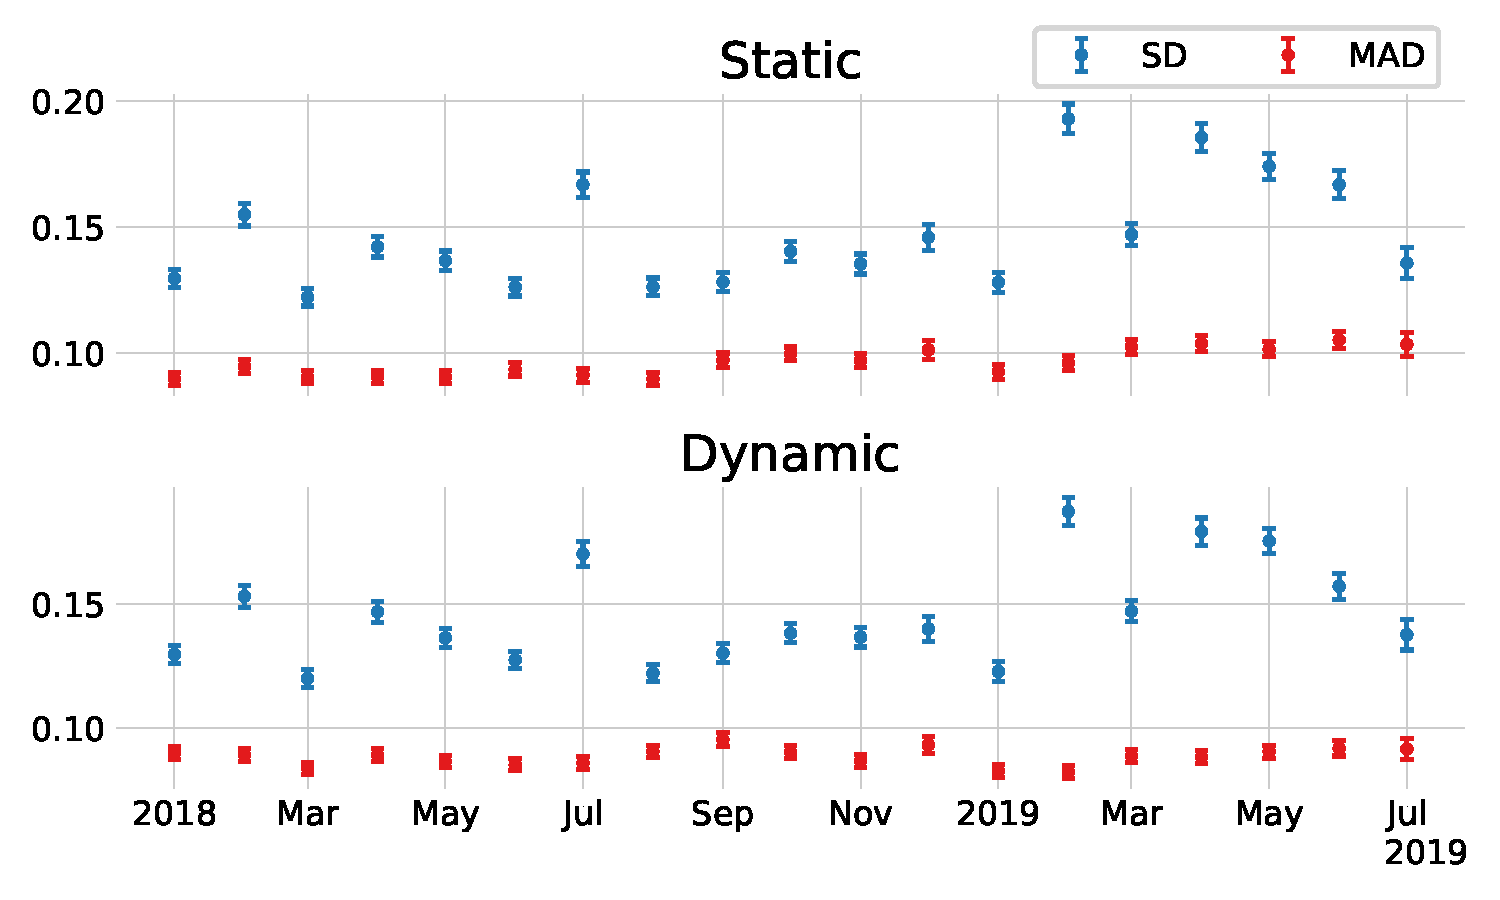
\includegraphics[width=0.99\textwidth, trim=10 15 10 10, clip]{figures/housing/Ejerlejlighed_v19_cut_all_Ncols_all_xgb_forecast_prediction_MAD.pdf}
  \caption[Standard Deviation and MAD of the Static and Dynamic XGB Forecasts]
          {Performance of 1-month forecasts for apartments sold in \num{2018} and \num{2019}. For both plots the XGB model is trained on data up to (but excluding) 2018. Top) The performance of the static model's prediction for both the \textcolor{blue}{standard deviation (SD)} and \textcolor{red}{MAD} of the $z$-scores. Bottom) Same as above, however, based on a dynamic model, i.e. a model which is retrained after every month to include the previous month's sales.} 
  \label{fig:h:forecast_MAD_SD}
\end{figure}

In the top subplot the results for the static forecast are shown, whereas the dynamic results are shown in the bottom subplot. The errorbars are calculated using the usual variance of the standard deviation:
\begin{equation}
  \sigma_\mu  = \frac{\sigma}{\sqrt{N}}, \quad \sigma_\sigma = \frac{\sigma}{\sqrt{2N}},
\end{equation}
where $\sigma_\mu$ is the standard deviation of the mean and $\sigma_\sigma$ is the standard deviation of the standard deviation\sidenote{That this estimator is biased does not matter since we are in the large $N$ limit, $N \sim 1000$.} \autocite{Barlow:0471922951}.
Notice the large fluctuations in the standard deviations over time compared to MADs which is an effect of MAD being a robust estimator. What is also interesting to note is that the MAD seems to increase over time for the static model, albeit slowly. In comparison, for the dynamic model this seem less pronounced. This figure not only shows the time dependence of the performance of the model, but also that the model is quite stable over time, at least for the dynamic model. 

Using the relative price predictions $\vec{z}$, we construct the Market Index, $\mathrm{MI}$. This is an index which measures the overall level of the Danish housing market based on the assumption that if the houses sold in a month are generally sold at a higher price than was predicted by the model, there can be two reasons for it: either the model was wrong or the market simply changed in the time span. With the latter assumption, the ratio between the prediction and the actual price of a residence is thus a measure of the market index:
\begin{equation}
  \begin{split}
    z_\mathrm{mi} &\equiv \frac{\hat{y}}{y} = 1 - \frac{\hat{y}-y}{y}  = 1-z \\
    \mathrm{MI}_\mathrm{mean} &= \mathrm{mean}(\vec{z}_\mathrm{mi}) \\
    \mathrm{MI}_\mathrm{median} &= \mathrm{median}(\vec{z}_\mathrm{mi}).
    \label{eq:h:market_index}
  \end{split}
\end{equation}
Here $\vec{z}_\mathrm{mi}$ is the vector of ratios between prediction and actual price, and the market index can then be estimated using either the mean $\mathrm{MI}_\mathrm{mean}$ or the median $\mathrm{MI}_\mathrm{median}$. The market indices for every month of the forecast described in the previous figure are shown in Figure~\ref{fig:h:forecast_MarketIndex}. In the top panel the market index is shown for the static model. Here the median $\mathrm{MI}_\mathrm{median}$  is consistently higher than \num{1}, around \SI{1}{\percent}. Compare this to the dynamic $\mathrm{MI}_\mathrm{median}$ in the lower plot which fluctuates around \num{1}. The mean $\mathrm{MI}_\mathrm{mean}$ is added to show its fluctuations are higher than the medians. 
\begin{figure}
  \centerfloat
  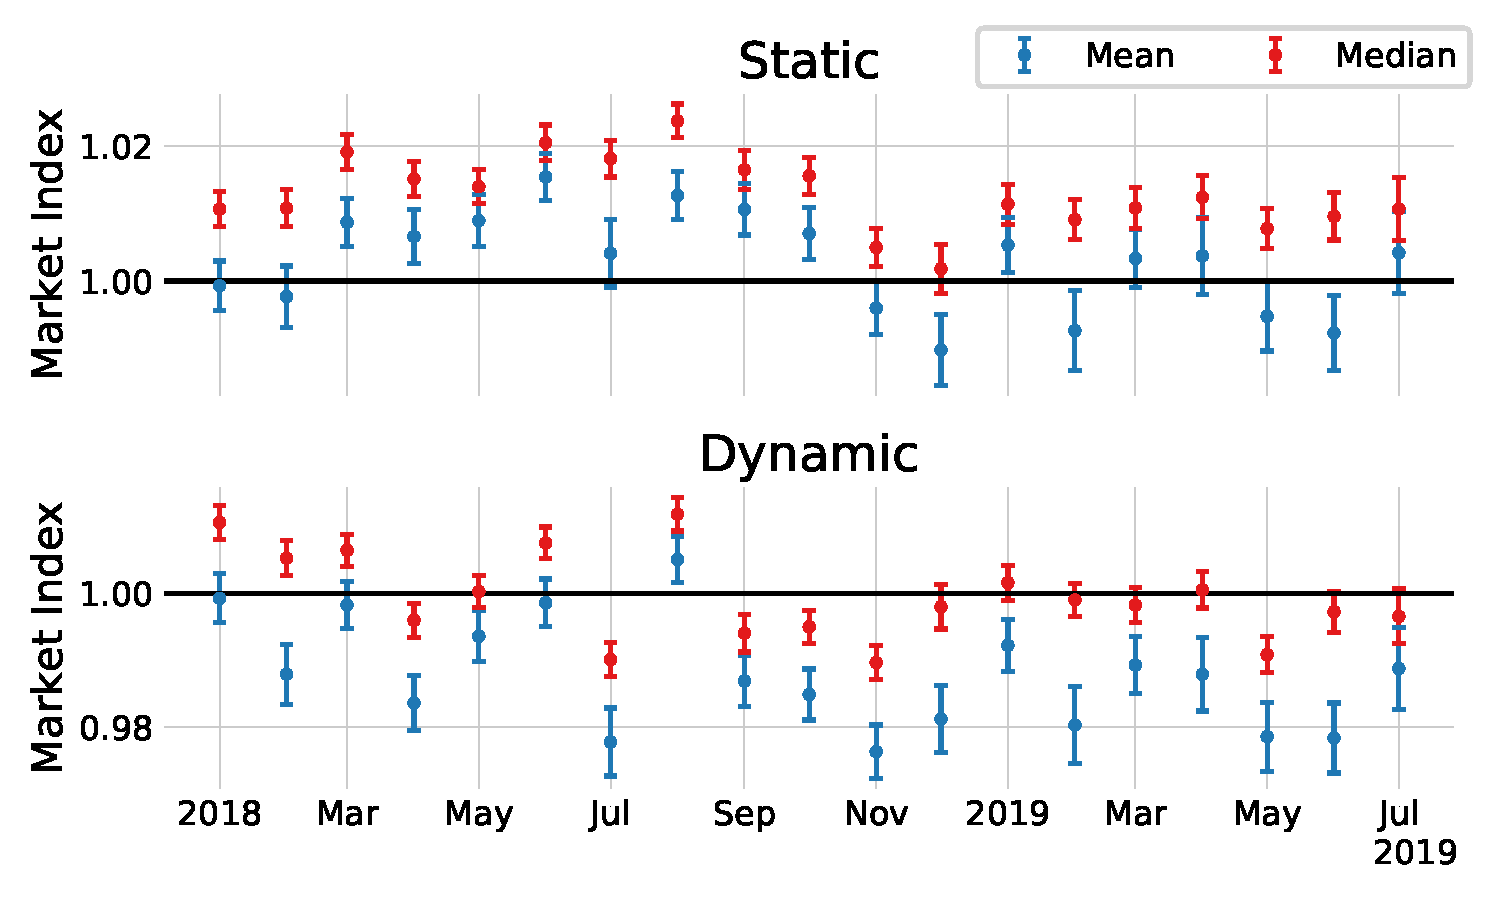
\includegraphics[width=0.99\textwidth, trim=10 15 10 10, clip]{figures/housing/Ejerlejlighed_v19_cut_all_Ncols_all_xgb_forecast_prediction_MarketIndex.pdf}
  \caption[Market Index based on the Static and Dynamic XGB Forecasts]
          {The Market Index as defined in equation \eqref{eq:h:market_index} for the static and dynamic 1-month forecasts for \num{2018} and \num{2019}. Plotted with using the \textcolor{red}{mean} in red and the \textcolor{blue}{median} in blue.} 
  \label{fig:h:forecast_MarketIndex}
\end{figure}

The final results for the model is seen in Table~\ref{tab:h:results_ejer} for owner-occupied apartments and in in Table~\ref{tab:h:results_villa} for one family houses. The MAD is around \SI{9}{\percent} for apartments and \SI{16}{\percent} for houses, which is still worse than the realtors' prediction, yet still acceptable for a model that does not have any variables describing the indoor conditions. For apartments around \SI{40}{\percent} of all the predictions are within $\pm \SI{5}{\percent}$ and more than \SI{90}{\percent} are within $\pm \SI{20}{\percent}$ which is similar to the performance of the professional automated property evaluations from e.g. \citet{bolighedBolighedUsikkerhedDatavurderingen}. The performance on the tight cuts is shown in Table~\ref{tab:h:results_ejer_tight} and \ref{tab:h:results_villa_tight}. 


\begin{table}
  \centerfloat
  \begin{tabular}{@{}lcccc@{}}
    {} &      MAD (\%) & $\leq 5\% (\%)$ &  $\leq 10\% (\%)$ &   $\leq 20\% (\%)$   \\
    \midrule
    Train & \num{7.83} & \num{47.90} & \num{75.74} & \num{93.97} \\
    Test  & \num{9.29} & \num{41.33} & \num{69.77} & \num{91.91} \\
    2019  & \num{9.89} & \num{38.85} & \num{66.76} & \num{90.04}    
  \end{tabular}
  \vspace{\abovecaptionskip}
  \caption[Performance Metrics for Apartments]{Performance metrics for the final housing model trained and evaluated on apartments.}
  \label{tab:h:results_ejer}
\end{table}


\begin{table}
  \centerfloat
  \begin{tabular}{@{}lcccc@{}}
    {} &      MAD (\%) & $\leq 5\% (\%)$ &  $\leq 10\% (\%)$ &   $\leq 20\% (\%)$    \\
    \midrule
    Train & \num{14.12} & \num{28.95} & \num{51.89} & \num{78.04}  \\
    Test  & \num{15.79} & \num{25.61} & \num{47.52} & \num{75.14}  \\
    2019  & \num{16.50} & \num{24.01} & \num{45.89} & \num{74.22}     
  \end{tabular}
  \vspace{\abovecaptionskip}
  \caption[Performance Metrics for Houses]{Performance metrics for the final housing model trained and evaluated on houses.}
  \label{tab:h:results_villa}
\end{table}


\FloatBarrier
\section{Model Inspection}
\label{sec:h:model_inspection}

One of the most important aspects of applying advanced machine learning methods, in addition to getting accurate predictions is to understand the model. As mentioned in \autoref{sec:ml:feature_importance}, it is possible to use SHAP values to inspect the trained model for both local predictions and for global feature importances $\phi_i^\mathrm{tot}$. An example of how to use SHAP to better understand a local prediction is seen in Figure~\ref{fig:h:shap_single_apartment}. Here the SHAP values for a particular sale are visualized as a bar chart where the green colors are positive values, red values negative values and the blue is the final prediction $\hat{y}$. Remember that for SHAP values the prediction is the sum of all of the SHAP values, see equation \eqref{eq:ml:additive_feature_attribution_method}. Here $\phi_0$ is the expectation value denoted as \code{Bias} in the plot. To show all \num{143} variables would make the figure excessively large, so two extra bins have been added: the \code{Overflow} bar which is the sum of the remaining positive SHAP values and likewise with \code{Underflow} for negative values. The sum of all the green and red bars adds up to $\hat{y}=\SI{6.86}{\Mkr}$ in this particular instance and the actual sold value was $y=\SI{6.35}{\Mkr}$. Thus, in cases where there is a large discrepancy between the predicted and actual sales prices, one use can use this tool to better understand why the prediction was estimated as it was. 

\begin{figure}[ht!]
  \centerfloat
  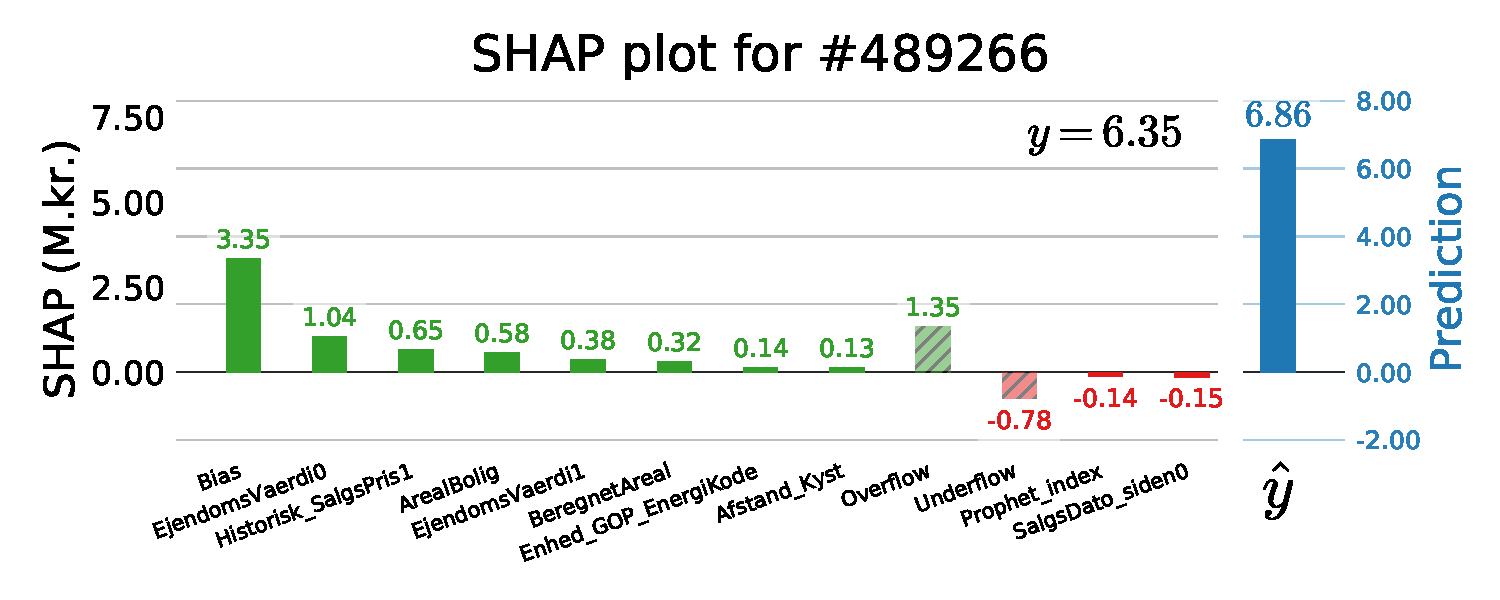
\includegraphics[width=0.99\textwidth, trim=15 15 10 40, clip]{figures/housing/Ejerlejlighed_v19_cut_all_Ncols_all_SHAP_fig_loc=489266.pdf}
  \caption[SHAP Prediction Explanation for Apartments]
          {Model explanation for XGB model for a specific apartment. The bars are the variables in the dataset that the model found most important sorted after their importance for this particular apartment. The bias bar refers to the expected value of the model, which is simply the mean of the training set which acts as the naive prediction baseline. The \q{cutoff positive (negative)} bars are the sum of the remaining positive (negative) values that are not shown. On the right hand side of the plot is the model prediction shown. The model prediction is the sum of all of the bars in the left par (\SI{6.86}{\Mkr} in this example). The \textcolor{red}{negative} values are shown in red, \textcolor{green}{positive} ones in green, and the \textcolor{blue}{prediction value} in blue. 
          } 
  \label{fig:h:shap_single_apartment}
\end{figure}

To get an overview of which variables are most important on a global\sidenote{Global here meaning for the entire dataset.} scale, $\phi_i^\mathrm{tot}$, see Figure~\ref{fig:h:shap_overview}. Here the variables are sorted according to the normalized $\phi_i^\mathrm{tot}$ which is shown in parentheses after each variable name. In the center of the plot is shown a dot-plot of the dataset plotted with the SHAP value on the abscissa and colored according to the feature value. 
The way to interpret this plot is as follows. Take a variable of interest, e.g. the area of the apartment \code{ArealBolig} with $\phi_\mathrm{ArealBolig}^\mathrm{tot}=\SI{5.35}{\percent}$. Every dot is a sale plotted as a function of their SHAP value with a spread such that the height corresponds to the SHAP distribution of that specific feature. For the area it can be seen that there is a long tail towards high SHAP values, however, most of the samples have a slightly negative SHAP values. The dots are colored according to their feature value and it can thus be seen that large apartments (red) are given a higher SHAP value than small apartments (blue); precisely as expected from the model. In contrary, when the the total days on market (\code{LiggetidSamlet}) is large it pushes the prediction in the negative direction. 

\begin{figure}[ht!]
  \centerfloat
  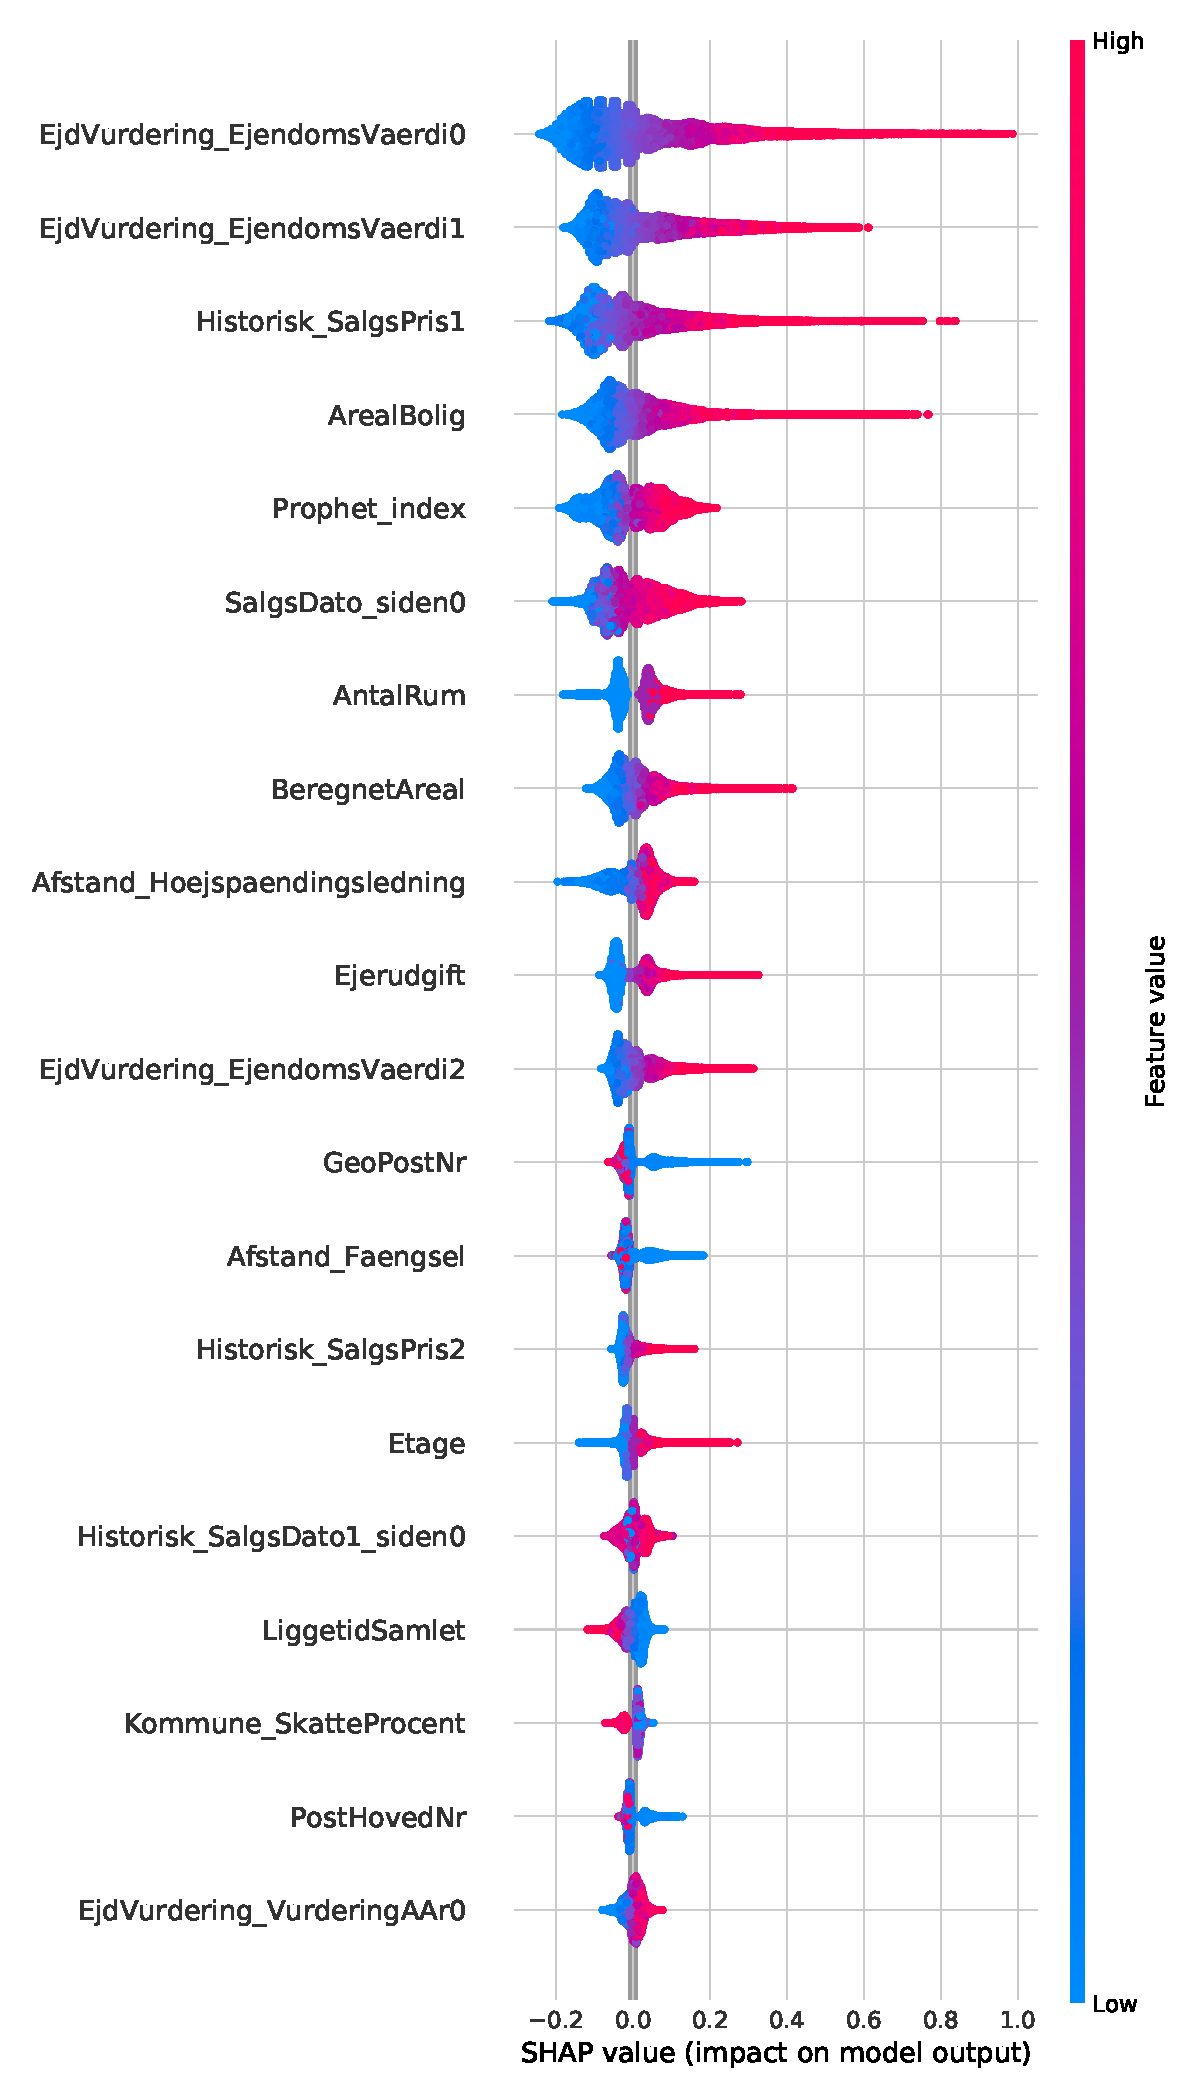
\includegraphics[width=0.9\textwidth, trim=0 0 0 1, clip]{figures/housing/Ejerlejlighed_v19_cut_all_Ncols_all_xgb_tight_SHAP_vals_summary.pdf}
  \caption[Feature importance of Apartments Prices]
          {Feature importance of apartment prices using the XGB-model. The feature importance is measured using SHAP values. The variables are sorted top to bottom according to their overall feature importance, i.e. the previous public property valuation \code{EjendomdsVaerdi0} is the most important single feature. Along the $x$-axis is the impact on model output, in this example the price in \si{\Mkr} This axes is colored by the value of the feature, from \textcolor{blue}{low} (blue) to \textcolor{red}{high} (red). In this particular example we see that high values of the previous public property valuation has high, positive impact on the model prediction -- exactly as expected. This is exactly opposite the total days on market described by the variable \code{LiggetidSamlet} where a high value has a negative impact.  
          } 
  \label{fig:h:shap_overview}
\end{figure}

The SHAP software \citep{lundbergConsistentIndividualizedFeature2018} not only allows for 1D dependencies to be gauged, it also allows for so-called \emph{interaction plots}. These plots shows the 2D-dependence between the variable and the SHAP value colored according to a second variable. Since the previous public property valuation (PPPV) (\code{EjendomdsVaerdi0}) is the most important of the features, the interaction plot of this variable is seen in Figure~\ref{fig:h:shap_overview_interaction}. 

Here the SHAP value of the \code{EjendomdsVaerdi0} is plotted as a function of \code{EjendomdsVaerdi0}. This plot shows that the higher the PPPV, the higher the model output. The colors show how this trend depends on time by the variable \code{SalgsDato_siden0} which is the number of days since January \nth{1} 2009 that the apartment was. The plot shows that if the apartment has a high PPPV then the newer sales has an even higher SHAP value then older sales, agreeing with the fact that the market has gone up since 2009. On the other hand, for low PPPV apartments the relationship with time is inverse, however, the effect is much smaller here. The SHAP software chose to color by \code{SalgsDato_siden0} since this is the variable which explains most of the variation for a given PPPV. 

\begin{figure}
  \centerfloat
  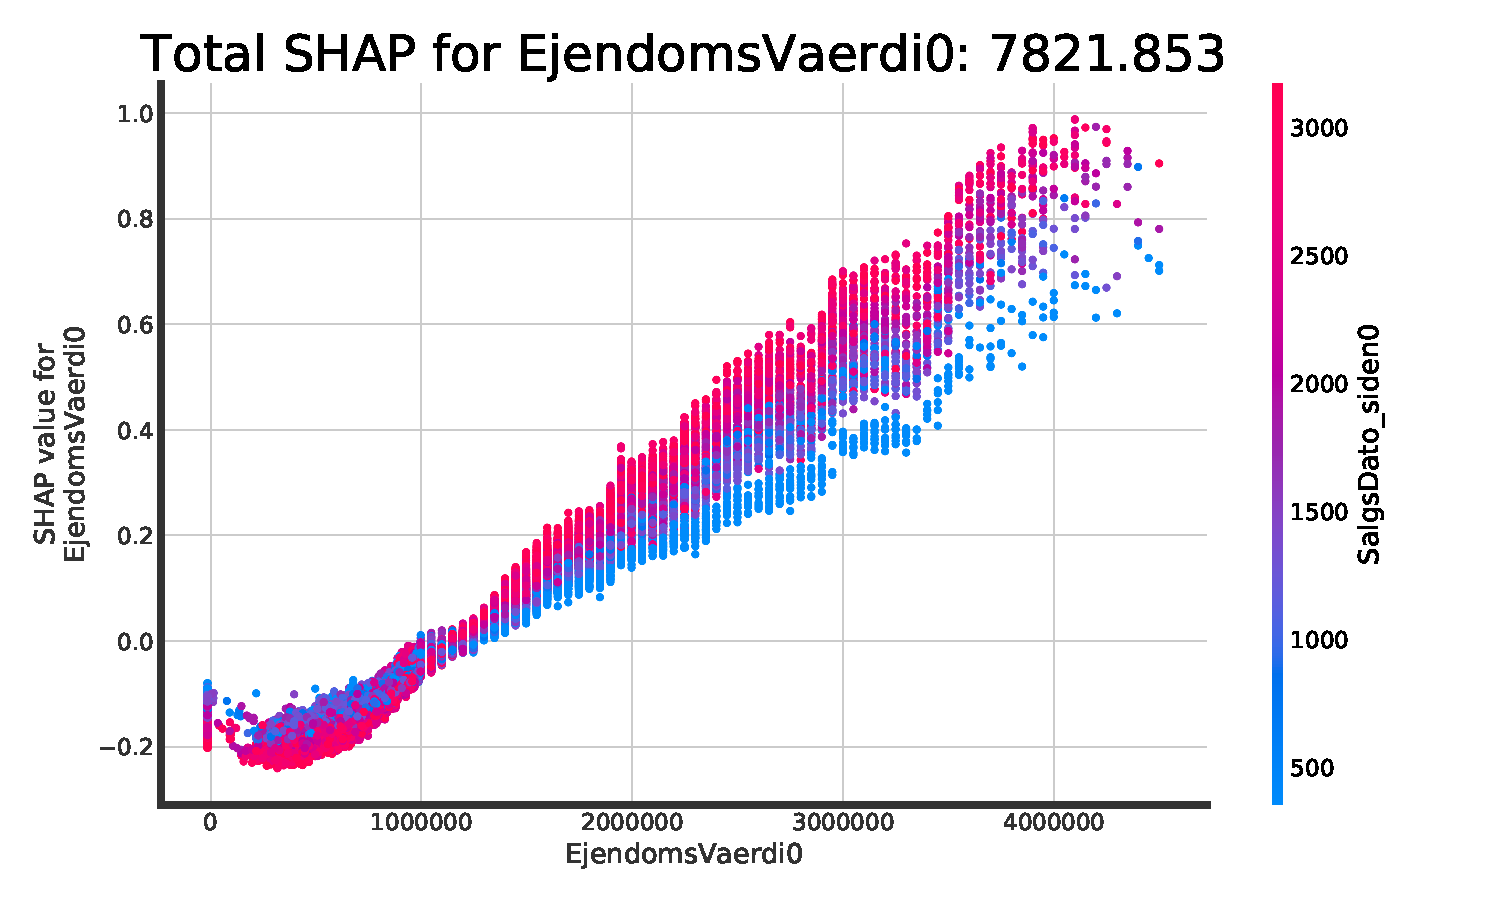
\includegraphics[draft=false, width=0.98\textwidth, trim=15 15 40 40, clip]{figures/housing/Ejerlejlighed_v19_cut_all_Ncols_all_xgb_tight_SHAP_vals_interaction_Vaerdi0.pdf}
  \caption[Feature Importance Interaction Plot for Apartments]
          {Interaction plot of the feature importances for the XGB model on apartments. Here shown for the previous public property valuation (\code{EjendomdsVaerdi0}) colored according to the sales date (\code{SalgsDato_siden0}).} 
  \label{fig:h:shap_overview_interaction}
\end{figure}

What can be concluded from this plot is that for apartments with a high PPPV and that were sold recently were sold for more than apartments with the same PPPV that were sold longer time ago; effectively the time dependence of sales prices. These interaction plots serves as helpful sanity checks to see that the model is actually learning reasonable relationships between the variables. 

\FloatBarrier
\section{Multiple Models}
\label{sec:h:multiple_models}

In addition to the XGBoost \autocite{chenXGBoostScalableTree2016} (XGB) BDT model, several other models were also tested. During the sub-project the LightGBM package \autocite{keLightGBMHighlyEfficient2017} (LGB), also a BDT model, was released and started gaining traction in the ML community, especially for large-scale data analysis. In comparison to XGBoost, LightGBM implements some extra binning and categorical assumptions that greatly speeds up the fitting process. It was trained in the same was as the XGBoost model with the same HPO-process and range for the hyperparameters. 

To compliment the BDTs models, a simple linear model (LIN) with $L_2$ loss, so-called \emph{ridge regression}, was fitted. Before the fit all of the NaNs were median-imputed which means that all invalid values were replaced with the median along each column. All the features were scaled\sidenote{Scaling of input features is generally an important preprocessing step for non-tree based ML models.} with a robust scaler from Scipy \autocite{virtanenSciPyFundamentalAlgorithms2019} in the $(25, 75)$ quantiles range and the regularization parameter was hyperparameter optimized. This linear model is quick and easy to both implement and fit, and can be seen as the simplest baseline model.

The $K$-nearest neighbors (KNN) algorithm was fitted to the data with a data preprocessing pipeline similar to the linear model with median imputation and robust scaling of the input features. For the HPO the number of neighbors, $K$, was optimized for together with the $p$-norm of the metric, $p \in \left\{ 1, 2\right\}$ (Manhattan, Euclidean, see also \autoref{subsec:regularization}).

Finally, support vector machines\sidenote{Known as support vector regression when applied to regression problems \autocite{awadSupportVectorRegression2015}.} (SVR) were used with the same preprocessing pipeline as the previous two methods and hyperparameter optimized for the $L_2$ regularization parameter $C$ and the kernel coefficient $\gamma$ for the radial basis function (RBF) kernel. 

\begin{figure*}[ht!]
  \centerfloat
  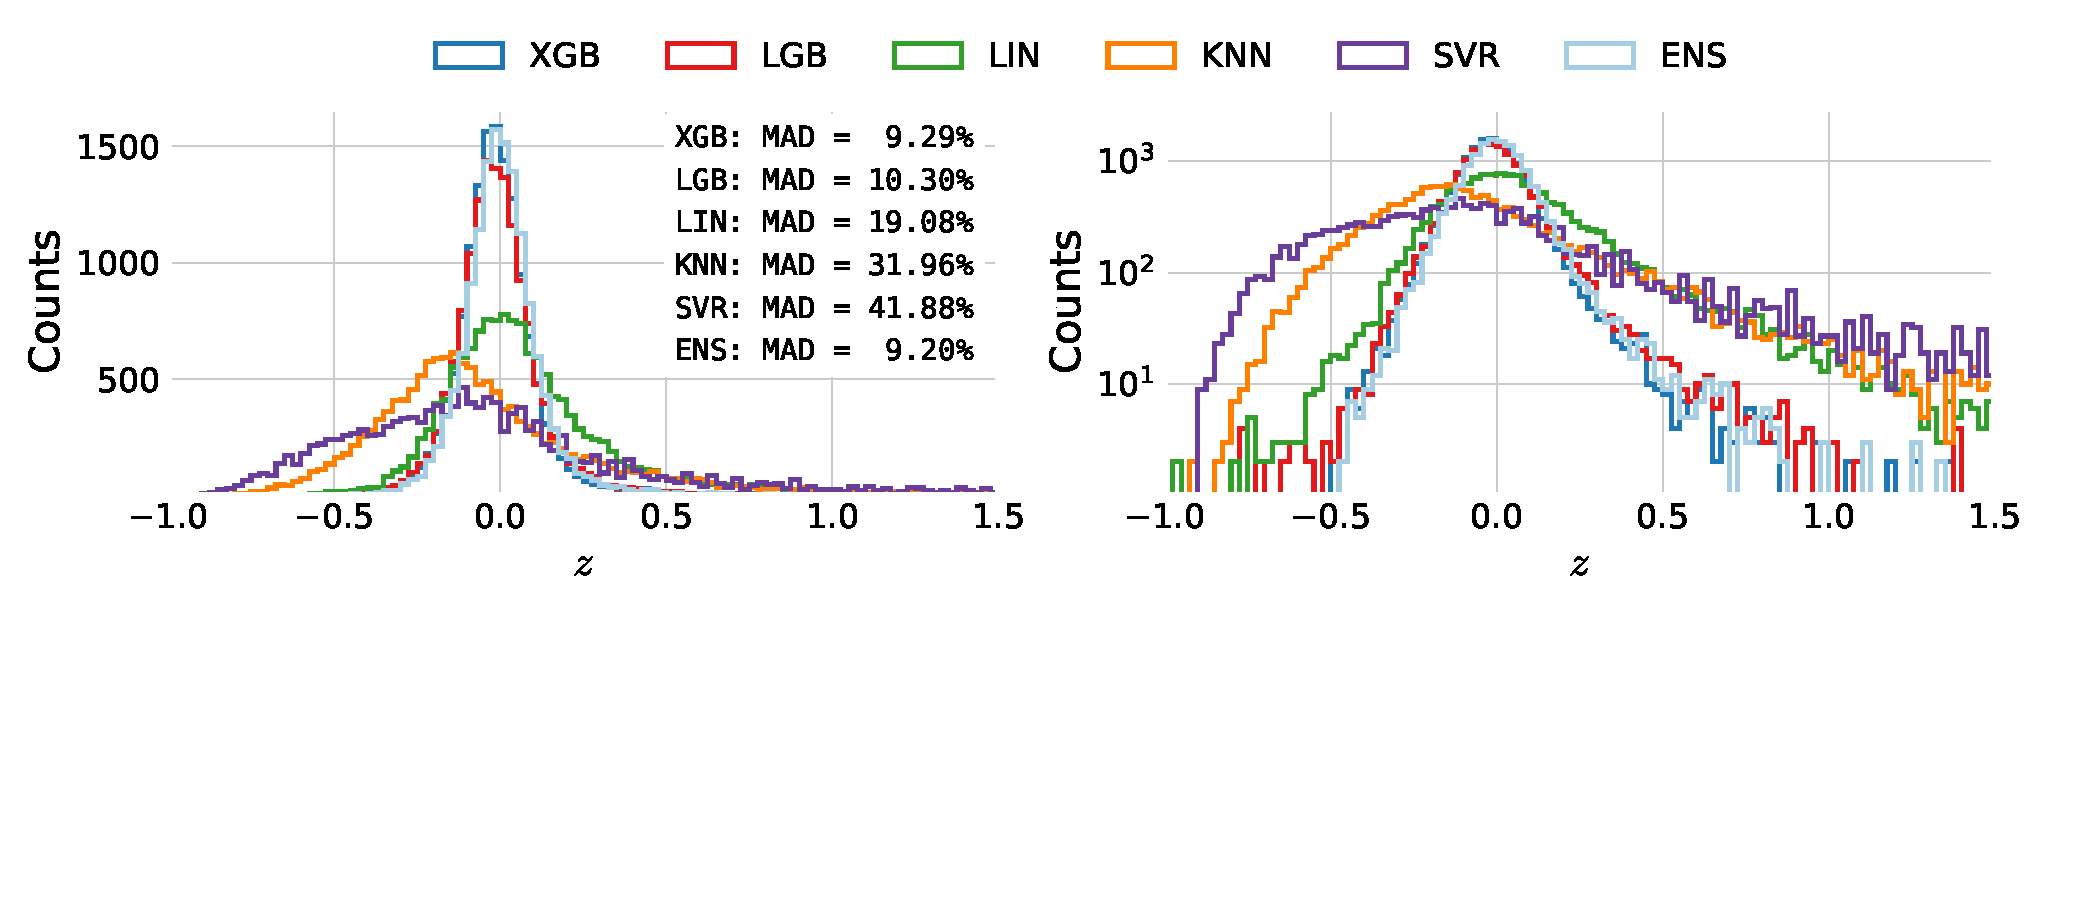
\includegraphics[draft=false, width=0.98\textwidth, trim=10 130 40 10, clip]{figures/housing/Ejerlejlighed_v19_cut_all_Ncols_all_all_models.pdf}
  \caption[Performance Comparison of Multiple Models for Apartments]
          {Distribution of the relative predictions $\vec{z}$ for apartments for the five different models and the ensemble model. The left plot shows the normal histogram (with a linear scale), whereas the right one has a log-scaled $y$-axis to better see the tails of the distributions. The MAD scores for the different models is further shown in the left plot.} 
  \label{fig:h:multiple_models}
\end{figure*}

The results for the five different models are shown in Figure~\ref{fig:h:multiple_models}, where the two subplots are the same up to a logarithmic scaling of the ordinate axis in the right plot. It is easily seen how XGBoost and LightGBM are the best-performing models together with the ensemble (ENS) of the different models, see paragraph below for further explanation. In the figure the MAD is also shown on the test set, which confirms the visual clue: that XGBoost performs best, followed by the ensemble model.


The five different models -- XGB, LGB, LIN, KNN, SVR -- should be able to each capture different parts of the hyperdimensional phase space and an ensemble of these models would thus be expected to be as good as or better than the best of the individual models. This kind of ensemble model is sometimes called \emph{super learner} in the statistics community \autocite{polleySuperLearnerPrediction2010,vanSuperLearner2007}. To make sure that the ensemble model is not just retraining on the training set, and thus end up overfitting, we follow the process from \citet{polleySuperLearnerPrediction2010}. Using cross-validation for time-series\sidenote{See \autoref{subsec:cross_validation}.} data with $10$ folds, the training data is split up into folds sorted by time. Each fold is fitted with all five models, and the prediction of the next fold is made for all five models. This is repeated for the remaining folds until one ends up with a matrix of predictions $\vec{Z} \in \mathbb{R}^{(N \times 5)}$ for $N$ training samples. Since all the folds in $\vec{Z}$ consists of predictions on unseen data\sidenote{The predictions for the very first fold is based on training data.} this prevents overfitting. The meta learner then fits $Z$ to the actual predictions of the training data $y$ in the usual way. The combination of a meta learner fitted to the predictions of individual models is called an ensemble model.

At first an XGBoost model was used as the meta learner yielding decent results, however, still performing worse than the single XGB model ($\mathrm{MAD} = \SI{9.57}{\percent}$). To better understand the issue, the meta learner was changed to a linear model which would basically just compute a weighted average of the different models:
\begin{equation}
  \label{eq:h:meta_learner}
  \Psi_\mathrm{meta}(\vec{x}) = \sum_{i=1}^5 \alpha_i \Psi_i(\vec{x}),
\end{equation}
where $\bm{\alpha}$ is a vector of the weights for the meta learner and $\Psi_i$ is each of the individual ML models. The linear model performed even worse than using XGB as the meta learner ($\mathrm{MAD} = \SI{10.48}{\percent}$), yet it was more transparent. During the debugging process it was realized that none of these models actually optimize the evaluation function, MAD, directly. The XGBoost model was trained using the Cauchy loss found earlier and the linear regression model a simple squared error loss. Since a simple weighted average should work as the meta learner \citep{polleySuperLearnerPrediction2010}, a custom algorithm for finding $\bm{\alpha}$ according to MAD was implemented.

Given the training data, the evaluation function as a function of $\bm{\alpha}$ was minimized using of the MINUIT algorithm \cite{1975CoPhC..10..343J} via the iminuit \cite{iminuit} Python interface. It yielded decent result, yet they were all very dependent on the initial parameter of the fit indicating many local minima. A scan over the 5-dimensional hyperspace in steps of $0.01$ was thus conducted and the result of this scan was used a the new initial parameter in the minimization routine. This yielded the following result:
\begin{equation}
  \bm{\alpha} = \begin{bmatrix*}[r] \alpha_\mathrm{LIN} \\  \alpha_\mathrm{KNN} \\ \alpha_\mathrm{SVR} \\ \alpha_\mathrm{XGB} \\ \alpha_\mathrm{LGB} \end{bmatrix*} = \begin{bmatrix*}[r] \SI{0.202}{\percent} \\  \SI{0.002}{\percent} \\\SI{0.001}{\percent} \\\SI{81.302}{\percent} \\\SI{20.002}{\percent} \end{bmatrix*}.
\end{equation}
The fact that it sums to more than \num{1} just corresponds to an overall scaling. When using the found $\bm{\alpha}$ in equation \eqref{eq:h:meta_learner}, one gets the ensemble model (ENS) shown in Figure~\ref{fig:h:multiple_models} with a $\mathrm{MAD} = \SI{9.20}{\percent}$. This value is the evaluation loss on the test set based on only the training data and outperforms all of the individual models. 

The paragraphs above refer to apartments, however, the intermediate results for houses showed the same pattern. The combined model along with its performance is shown in Figure~\ref{fig:h:multiple_models_villa}

\section{Discussion}
\label{sec:h:discussion}

The subproject of estimating housing prices has focussed a lot on experimenting with different machine learning models and how to optimize them. As shown in the previous sections, the choice of ML model is by far the most important. Actually, the gain from HPO is quite small, especially considering the amount of time spent on it\sidenote{Not only user-time programming it, but also the computational ressources spent.}. With the dataset at hand, decent results were made, however, they were nowhere near the performance of the realtors' predictions. 

There are two main reasons for this, the first being that realtors are educated within this field and thus has developed the skills required for estimating the price of a house over many years of hard work. The second reason is the fact that the realtor has access to a lot more information than the ML models have. We are not in possession of any \emph{indoor} variables as we call it. The area of the house, the number of rooms, the name of the street, and the distance to a highway are all variables that are in the data set but none of them describe the overall quality of the house, the maintenance level, the age of the kitchen or bathroom. These features are invisible to the ML model. 

During the project it was investigated how to get access to these variables. At first the online images from each sale was suggested, however, it turned out that Boligsiden only have the right to use them while a residence is for sale; when it is sold all rights return to the photographer. The images are not the only thing that provide more information about the condition of the residence, also the descriptions does that. 

The descriptions turned out to be available for most of the sales and was investigated for a short period. At that time of the project, the MAD for (a subset of the) apartments was around $\pm \SI{14}{\percent}$ and $\pm \SI{20}{\percent}$ for houses. By using methods from the big natural language processing (NLP) community with in the field of machine learning, it was possible to reduce the MAD to around $\pm \SI{12}{\percent}$ and $\pm \SI{15}{\percent}$ for apartments and houses respectively. From the improvement in performance it is noticeable how apartments in general are much more uniform compared to houses where the \q{inside} is more decisive regarding the price. 

\begin{figure}[h!]
  \centering
  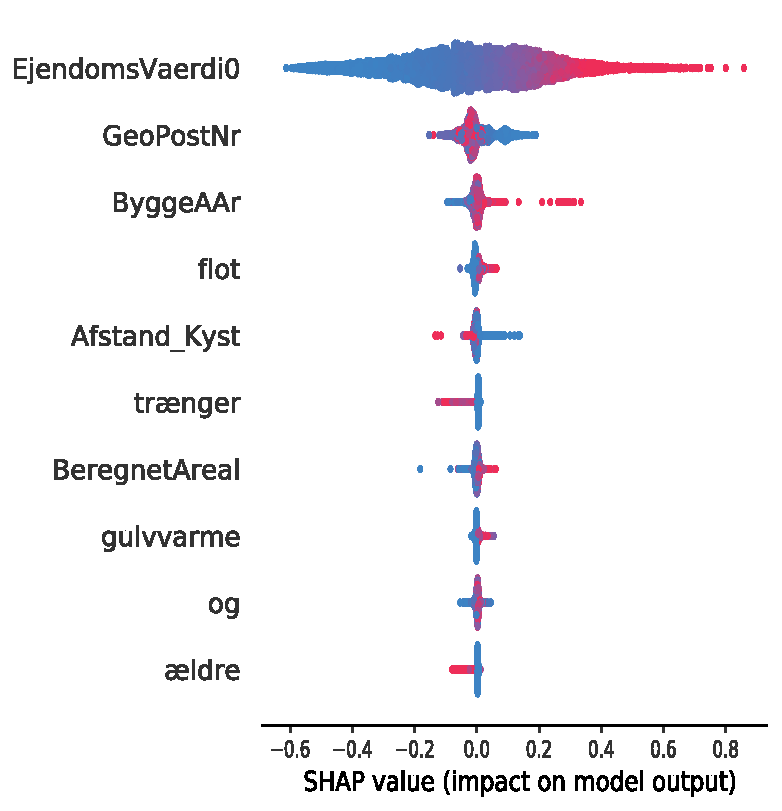
\includegraphics[width=0.8\textwidth]{figures/housing_text/villa_tfidf.pdf}
  % \caption[SHAP plot villa TFIDF XXX]{SHAP plot villa TFIDF XXX.}
  \caption[Feature Importance of Villas With Descriptions]
          {Feature importance of villas when the descriptions are also used. The variables are sorted top to bottom according to their overall feature importance, i.e. the previous public property valuation \code{EjendomdsVaerdi0} is the most important single feature. Along the $x$-axis is the impact on model output, in this example the price in \si{\Mkr} This axes is colored by the value of the feature, from \textcolor{blue}{low} (blue) to \textcolor{red}{high} (red). In this particular example we see that high values of the previous public property valuation has high, positive impact on the model prediction -- exactly as expected. This is in contrast to the word \q{requires} (\colorbox{light-gray}{\texttt{trænger}}) where a high value has a negative impact.} 
  \label{fig:h:shap_text}
\end{figure}

The methods for translating the text to numerical variables decipherable by classical ML models were for instance simple \emph{bag of words} (BOW) models and term \emph{Term Frequency, Inverse Document Frequency} (TF-IDF) but also slightly more advanced statistical tools such as \emph{Latent Dirichlet Allocation} (LDA). An old example of the learnt text model is seen in Figure~\ref{fig:h:shap_text} where a housing-based model was trained with the five numerical variables\sidenote{With the Danish names: \code{Ejendomsvaerdi0}, \code{GeoPostNr}, \code{ByggeAAr}, \code{Afstand_Kyst}, and \code{BeregnetAreal}.}: the PPPV, postal code, year of construction, distance to shore, and the weighted area. and the text descriptions (encoded with TF-IDF). 

The summary of the trained model is as a SHAP plot in Figure~\ref{fig:h:shap_text}. As expected, the most important features are the numerical ones, however, the word \code{flot} (\q{pretty}) was in top five. The model also learnt that \code{flot} has a positive impact on the price compared to \colorbox{light-gray}{\texttt{trænger}} (\q{requires}) which has a negative impact.
% \code{Ejendomsvaerdi0} (PPPV), \code{GeoPostNr} (postal code), \code{ByggeAAr} (year of construction), \code{Afstand_Kyst} (distance to shore), and \code{BeregnetAreal} (weighted area) 

The descriptions turned out to be more time-consuming to extract for Boligsiden and along with the fact that overall deadline was quickly approaching, the remaining time was focussed on the main part of the project, the quark gluon discrimination. Given more time, the text analysis would definitely be the first step for further improving the accuracy and precision of the price predictions. 

Another step would be to apply more modern deep learning\sidenote{Basically advanced neural networks with many layers.} methods. These methods were briefly experimented with in the initial stages of this subproject but showed inferior performance compared to BDTs. It is generally accepted in the ML community (with some modifications) that neural networks underperform, or at least not outperform, classic ML methods on structured \sidenote{In general data that can be described by a spread sheet, i.e. has a well-defined number of variables and observations which is why it is also known as \emph{tabular data}.} data \autocite{klambauerSelfNormalizingNeuralNetworks2017}. Most often they have the inherent complexity needed to perform as well as other ML methods, however, this requires extensive architecture optimization, or, in short; the hypothesis space for neural networks is much larger than for classical ML methods and thus requires more care to avoid overfitting.

\section{Conclusion}
\label{sec:h:conclusion}

XXX \TODO